\documentclass[fontsize=12pt, paper=a4, titlepage=on, BCOR=8mm, DIV=15, twoside, openany]{scrbook}

\usepackage{graphicx} % Required for inserting images
\usepackage[T1]{fontenc} %Notwendig um Umlaute benutzen zu können 
\usepackage[ngerman]{babel} %import vom deutschen Sprachpaket
\usepackage{microtype} %Kleine Variationen im Textabstand um Silbentrennung zu reduzieren
\usepackage{lmodern}
\usepackage{hyphenat} %Für manuelle Silbentrennung
\usepackage[headsepline, plainheadsepline, markcase=used]{scrlayer-scrpage}     %Seitendesign einstellungen
\usepackage{ziffer} %deutsche dezimaltrennung als ,
\usepackage{listings} %Für Code auszüge
\usepackage{xcolor} %Für Farbgebungen
\usepackage{scrhack}
\usepackage{hyperref}
\usepackage{caption}
\usepackage{bookmark}
\usepackage{amsmath}
\usepackage{amssymb}
\usepackage{geometry}
\usepackage{blindtext}
\usepackage[acronym]{glossaries}
\usepackage[backend=biber, sortcites, citestyle=numeric]{biblatex}
\usepackage[autostyle]{csquotes}
\usepackage{todonotes}
\usepackage{nomencl}

\addbibresource{bib/bibF.bib}

\captionsetup{skip=10pt}

\renewcommand{\familydefault}{\sfdefault}       %Font übernehmen für das ganze Dokument

\graphicspath{{img/}} % Ordner für Bilder Festlegen

%\bibliographystyle{ieeetr}

\makeglossaries

\makenomenclature
\renewcommand{\nomname}{Mathematische Notation}
\setlength{\nomlabelwidth}{3cm}
% Befehle für unterschiedliche Formatierungen
%\newcommand{\nomupbold}[1]{\mathrm{\mathbf{#1}}} % Tensoren fett und gerade
\newcommand{\nomvec}[1]{\vec{#1}} % Spaltenvektor
\newcommand{\nomvecT}[1]{\vec{#1}^\mathrm{T}} % Zeilenvektor
\newcommand{\nommat}[1]{\boldsymbol{#1}} % Matrix


\pagestyle{scrheadings} %Seitenstil preset
\clearpairofpagestyles  %Seitenzahlen aus der Fußzeile löschen
\chead{\headmark}       %Kapitelüberschriften außen in der Kopfzeile
\ohead*[\pagemark]{\pagemark}   

\geometry{
  inner=2.5cm, % Größerer innerer Rand für die Bindung
  outer=1.5cm, % Kleinerer äußerer Rand
  top=0.6cm,
  bottom=3cm,
  headsep=15pt,
  includehead
}

% Umgebungsfarben für Codeausschnitte
\definecolor{codegreen}{rgb}{0,0.6,0}
\definecolor{codegray}{rgb}{0.5,0.5,0.5}
\definecolor{codepurple}{rgb}{0.58,0,0.82}
\definecolor{backcolour}{rgb}{0.95,0.95,0.92}
\lstdefinestyle{mystyle}{
    backgroundcolor=\color{backcolour},   
    commentstyle=\color{codegreen},
    keywordstyle=\color{magenta},
    numberstyle=\tiny\color{codegray},
    stringstyle=\color{codepurple},
    basicstyle=\ttfamily\footnotesize,
    breakatwhitespace=false,         
    breaklines=true,                 
    captionpos=b,                    
    keepspaces=true,                 
    numbers=left,                    
    numbersep=5pt,                  
    showspaces=false,                
    showstringspaces=false,
    showtabs=false,                  
    tabsize=2
}

\lstset{style=mystyle}

%Neudefinition des \mainmatter befehls, um bei Aufruf die letze Seitenzahl des 
%Frontmatters zu speichern, um beim Backmatter wieder drauf zurückgreifen zu können
\makeatletter
\newcounter{savedfrontmatterpage}
\renewcommand{\mainmatter}{%
  \cleardoublepage
  \setcounter{savedfrontmatterpage}{\value{page}}%
  \@mainmattertrue
  \pagenumbering{arabic}%
  \clearpairofpagestyles
  \ohead{\headmark}
  \ofoot*[\pagemark]{\pagemark}
}

%Neudefiniton des backmatter-Befehls, um bei AUfruf die Seitenzahl auf die letzte Seitenzahl des Frontmatters zurückzugreifen
\renewcommand\backmatter{%
  % Prüft, ob die Seite ungerade ist (rechte Seite)
  \ifodd\value{page}%
    \cleardoublepage % Wechselt zur nächsten rechten Seite, wenn aktuell auf einer rechten Seite
  \else
    \clearpage % Nur ein einfacher Seitenumbruch, wenn auf einer linken Seite
  \fi
  \@mainmatterfalse
  \pagenumbering{Roman}%
  \setcounter{page}{\value{savedfrontmatterpage}}%
  \clearpairofpagestyles
  \chead{\headmark}                                                               %Kapitelüberschriften außen in der Kopfzeile
  \ohead*[\pagemark]{\pagemark}                                                    %Seitenzahlen innen in der Kopfzeile
}
\makeatother

\newcommand{\theauthor}{Leon Grude}
\newcommand{\thetitle}{Entwicklung eines Moduls zur automatischen Klassifikation von Verhaltensweisen von Mastputen mittels Machine-Learning-Methoden}
\newcommand{\thedate}{02.02.2024}

\newcommand{\emptyFigure}[2]{
    \begin{figure}[ht]
        \centering
        \frame{
\includegraphics[width=\textwidth, height=3cm]{img/EMPTY.png}}
        \caption{#1}
        \label{#2}
    \end{figure}
}

% Command to create a glossary entry with correspondent acronym.
% Args : 1: acronym/name, 2: long name, 3: description
\newcommand{\newglossaryentrywithacronym}[3]{
    %%% The glossary entry the acronym links to   
    \newglossaryentry{#1_gls}{
        name={#1},
        long={#2},
        description={#3}
    }

    % Acronym pointing to glossary
    \newglossaryentry{#1}{
        type=\acronymtype,
        name={#1},
        description={#2},
        first={#2 (#1)\glsadd{#1_gls}},
        see=[Glossary:]{#1_gls}
    }
}

\begin{filecontents}{emptybib}
@article{EMPTYCITE,
 author = {None, None},
 year = {0000},
 title = {None},
}
\end{filecontents}

\addbibresource{emptybib}

\newcommand{\dubpar}{\vspace{1cm}}

\newcommand{\gfuss}[1]{\glqq#1\grqq}
%%%%%%%%%%%%%%%%%%%%%%%%%%%%%%%%%%%%%%%%%%%%%%%%%%%%%%%%%%%%%%%%%%%%
%-----------------------Allgemeines---------------------------------
%%%%%%%%%%%%%%%%%%%%%%%%%%%%%%%%%%%%%%%%%%%%%%%%%%%%%%%%%%%%%%%%%%%%

\newglossaryentry{Modul}
{
        name=Modul,
        description={In der Informationstechnik ist ein Modul ein Baustein eines Systems, welcher sich einfach austauschen lässt. Es kapselt Funktinoalität in einem eigenständigen Block. Module sind Systemelemente, welche in sich selbst Systeme sind}
}

\newglossaryentry{System}
{
        name=System,
        description={Eine eindeutig abgegrenzte Einheit bestehend aus verschiedenen Subsystemen und Systemelementen sowie deren Verknüpfungen}
}

\newglossaryentry{Frame}
{
        name=Frame,
        description={Im Kontext von Videos bezieht sich Frame auf ein einzelnes Bild in einer Reihe von Bildern, die zusammen ein Video bilden.}
}

\newglossaryentry{Mid-Level Aufgabe}
{
        name=Mid-Level Aufgabe,
        description={Mid-Level Aufgaben sind Tätigkeiten oder Prozesse, die zwischen Low-Level- und High-Level-Aufgaben notwendig sind. Mid-Level-Aufgaben fokussieren sich auf die Integration und Koordination zwischen diesen beiden Ebenen, um eine effiziente Ausführung von Anwendungen zu gewährleisten.}
}

\newglossaryentry{Ereignis}
{
        name=Ereignis,
        description={Im Kontext dieser Arbeit bezieht sich ein Ereignis auf eine spezifische Verhaltensweise, die innerhalb eines definierten Zeitraums auftritt.}
}

\newglossaryentry{Brownsche Bewegung}
{
        name=Brownsche Bewegung,
        description={Ist eine zufällige Bewegung von Teilchen in einer Flüssigkeit oder in einem Gas, die auf Stöße mit den Molekülen des Mediums zurückzuführen ist. Die Bewegungen sind zufällig.}
}

\newglossaryentrywithacronym
{IoU}
{Intersection over Union}
{Das Verhältnis des Überlappungsbereichs zwischen der vorhergesagten Bounding-Box und der wahren Bounding-Box zum Gesamtvereinigungsbereich beider Boxen.}

\newglossaryentry{Just-in-time}
{
        name=Just-in-time Kompilierung,
        description={Bei einer Kompilierung wird ein Computerprogramm in maschinenlesbaren Code übersetzt. Dies geschieht üblicherweise vor der Programmausführung. Bei Just-in-time Kompilierung erfolgt die Kompilierung während der Ausführung, in dem Moment wo der zu kompilierende Programmabschnitt aufgerufen wird.}
}

\newglossaryentry{Overhead}
{
        name=Overhead,
        description={Bezeichnet zusätzlichen Rechenaufwand, der durch die Ausführung einer bestimmten Aufgabe entsteht, welche nicht direkt zur eigentlichen Funktionalität beiträgt.}
}


\newglossaryentry{Echtzeitfähigkeit}
{
        name=Echtzeitfähigkeit,
        description={Echtzeitfähigkeit bedeutet, dass ein System innerhalb einer festgelegten Zeitspanne auf den Eingang reagiert. Das Ergebnis muss nach einer vorgegebenen Dauer feststehen \cite{Scholz.2005}.}
}

%%%%%%%%%%%%%%%%%%%%%%%%%%%%%%%%%%%%%%%%%%%%%%%%%%%%%%%%%%%%%%%%%%%%
%-----------------------MOT Allgemein-----------------------------------------
%%%%%%%%%%%%%%%%%%%%%%%%%%%%%%%%%%%%%%%%%%%%%%%%%%%%%%%%%%%%%%%%%%%%

\newglossaryentrywithacronym
{MOT}
{Multi-Object Tracking}
{Ein Teilbereich des maschinellen Sehens, das darauf abzielt, mehrere Objekte in einem Video zu detektieren, lokalisieren und über die Zeit so zu assoziieren, dass die Identitäten konstant zugeordnet bleiben \cite{HOTA}.}

\newglossaryentry{Tracking}
{
name=Tracking,
description={Die Verfolgung und der Bewegung von Objekten über die Zeit.}
}

\newglossaryentry{Detektionsbasiertes Tracking}
{
name=Detektionsbasiertes Tracking,
description={Ein Ansatz im Multi-Object Tracking, bei dem Objekte zunächst in jedem Frame detektiert und anschließend über die Zeit hinweg verfolgt werden.}
}

\newglossaryentry{Detektion}
{
name=Detektion,
description={Das Erkennen und Markieren von Objekten in Frames, vorallem im Kontext des Multi-Objekt Trackings.}
}

\newglossaryentry{Assoziation}
{
name=Assoziation,
description={Die Zuordnung von erkannten Objekten über aufeinanderfolgende Frames, um die  Identitäten der Objekte konstant zu halten. Vorallem im Kontext des Multi-Objekt Trackings verwendet.}
}

\newglossaryentry{Lokalisation}
{
name=Lokalisation,
description={Die Bestimmung der genauen Position eines Objekts innerhalb eines Frames, oft ausgedrückt durch Koordinaten oder eine Bounding Box. Vorallem im Kontext des Multi-Objekt Trackings verwendet.}
}

\newglossaryentry{Offline Tracking}
{
name=Offline Tracking,
description={Ein Tracking-Verfahren, bei dem alle Daten vor der Verarbeitung zur Verfügung stehen.}
}

\newglossaryentry{Online Tracking}
{
name=Online Tracking,
description={Ein Tracking-Verfahren, das die Daten sequenziell verarbeitet, ohne auf zukünftige Frames zuzugreifen. Ideal für Echtzeitanwendungen.}
}

\newglossaryentry{Trajektorie}
{
name=Trajektorie,
description={Die Bewegungslinie, die ein Objekt über die Zeit in einem Raum durchläuft. Eine Trajektorie ist eine Sequenz von Positionen des Objekts.}
}

\newglossaryentry{Bounding Box}
{
name=Bounding Box,
description={Ein rechteckiger Rahmen, der verwendet wird, um die Position und die Größe eines Objekts zu definieren.}
}

\newglossaryentry{Ground Truth}
{
name=Ground Truth,
description={Die genauen Detektionen, Positionen und Assoziationen der Objekte in einem Ereignis. Die Ground Truth dient als Refernzen für die Evalutaion von Multi-Object Tracking Systemen.}
}


%%%%%%%%%%%%%%%%%%%%%%%%%%%%%%%%%%%%%%%%%%%%%%%%%%%%%%%%%%%%%%%%%%%%
%-----------------------MOT Fehler-----------------------------------------
%%%%%%%%%%%%%%%%%%%%%%%%%%%%%%%%%%%%%%%%%%%%%%%%%%%%%%%%%%%%%%%%%%%%


%%%%%%%%%%%%%%%%%%%%%%%%%%%%%%%%%%%%%%%%%%%%%%%%%%%%%%%%%%%%%%
%%%%%%%%%%%%%%%%%%%%%%%%%%%%%%%%%%%%%%%%%%%%%%%%%%%%%%%%%%%%%%
%%%%%%%%%%%%%%%%%%%%%%%%%%%%%%%%%%%%%%%%%%%%%%%%%%%%%%%%%%%%%%
%%%%%%%%%%%%%%%%%%%%%%%%%%%%%%%%%%%%%%%%%%%%%%%%%%%%%%%%%%%%%%
\newglossaryentrywithacronym
{EP}
{Echt positive Detektion}
{Es ist eine korrekte Detektion. Eine echt positive Detektion tritt auf, wenn ein MOT System ein Objekt detektiert, welches wirklich existiert.}

\newglossaryentrywithacronym
{FP}
{Falsch positive Detektion}
{Ein Detektionsfehler. Eine falsch positive Detektion tritt auf, wenn ein MOT System ein Objekt detektiert, welches in Wirklichkeit nicht da ist.}

\newglossaryentrywithacronym
{FN}
{Falsch negative Detektion}
{Ein Detektionsfehler. Eine falsch negative Detektion tritt auf, wenn ein MOT System ein Objekt, welches in Wirklichkeit da ist, nich detektiert.}

\newglossaryentry{Fragmentation}
{
name=Fragmentation,
description={Ein Assoziationsfehler. Eine Fragmentation tritt auf, wenn ein Objekt in den vergangenen Frames eine ID \(a\) zugewiesen bekommen hat und im aktuellen Frame eine ID \(b\) erhält. Die korrekte Trajektorie des Objektes besteht aus dem Fragment mit der ID \(a\) und \(b\). Eine unvollständige Trajektorie zählt ebenfalls als Fragmentation.}
}

\newglossaryentry{Merging Fehler}
{
name=Merging Fehler,
description={Ein Assoziationsfehler. Ein Merging Fehler ist das Gegenstück zur Fragmentation. Er tritt auf, wenn zwei Objekte, Objekt \(a\) und Objekt \(b\) vom System die gleiche ID erhalten. Das System hält die beiden Objekte für ein einzelnes Objekt.}
}

\newglossaryentry{Lokalisationsfehler}
{
name=Lokalisationsfehler,
description={Eine Abweichung von der genauen Position des detektierten Objekts.}
}

\newglossaryentrywithacronym
{IDSW}
{Identity Switch}
{Fehler eines MOT Systems. Ein Identity Switch tritt auf, wenn sich die Identifikationsnummer (ID) eines Objektes ändert, obwohl sie konstant bleiben sollte. Dabei berücksichtigt eine Identity Switch jedoch keine unvollständigen Trajektorie. Wird eine Trajektorie
abgebrochen, obwohl sich das Objekt weiter im Ereignis befindet, gibt es keine ID die sich
ändern kann.}

%%%%%%%%%%%%%%%%%%%%%%%%%%%%%%%%%%%%%%%%%%%%%%%%%%%%%%%%%%%%%%%%%%%%
%-----------------------MOT Metriken-----------------------------------------
%%%%%%%%%%%%%%%%%%%%%%%%%%%%%%%%%%%%%%%%%%%%%%%%%%%%%%%%%%%%%%%%%%%%

\newglossaryentrywithacronym
{MOTP}
{Multiple Object Tracking Precision}
{Teil der \textit{\acrshort{CLEAR} \gls{MOT}} Metriken. Es ist ein Maß für die Präzision, mit der Lokalisation eines MOT Systems. MOTP berechnet sich über den Mittelwert der \(IoU\) aller echt positiven Detektionen.}

\newglossaryentrywithacronym
{MOTA}
{Multiple Object Tracking Accuracy}
{Teil der \textit{\acrshort{CLEAR} \gls{MOT}} Metriken. Es ist ein Maß für die Gesamtgenauigkeit eines MOT-Systems, das die Anzahl der echt positiven Detektionen, die falsch negativen Detektionen und die IDSWs berücksichtigt.}

\newglossaryentrywithacronym
{MODA}
{Multiple Object Detection Accuracy}
{Teil der \textit{\acrshort{CLEAR} \gls{MOT}} Metriken. Es ist ein Maß für die Genauigkeit der Detektion. Die Berechnung erfolgt wie bei MOTA, nur ohne die Berücksichtigung der IDSWs.}

\newglossaryentry{IDF1}
{
name=IDF1,
description={Es ist ein Maß für die Gesamtgenauigkeit eines MOT-Systems. Sie misst das Verhältnis der korrekt assoziierten Detektionen zur Gesamtzahl der System-Detektionen und der Anzahl der Ground Truth Detektionen.}
}

\newglossaryentrywithacronym
{HOTA}
{Higher Order Tracking Accuracy}
{Eine fortgeschrittene Metrik für die Bewertung von MOT Systemen, die sowohl die Detektions- als auch die Assoziationsgenauigkeit berücksichtigt. HOTA ist darauf ausgerichtet, die Teilkomponenten eines MOT Systems fair zu bewerten. Es ermöglicht eine ausführliche Systemanalyse mittels Submetriken.}

\newglossaryentrywithacronym
{DetA}
{Detection Accuracy}
{Submetrik der HOTA Metrik. Es ist ein Maß für die Gesamtgenauigkeit der Detektion. DetA berücksichtigt den Einfluss von unterschiedlichen Detektionsfehlern gleichwertig.}

\newglossaryentrywithacronym
{AssA}
{Association Accuracy}
{Submetrik der HOTA Metrik. Es ist ein Maß für die Gesamtgenauigkeit der Assoziation. AssA berücksichtigt den Einfluss von unterschiedlichen Assoziationsfehlern gleichwertig.}

\newglossaryentrywithacronym
{DetRe}
{Detection Recall}
{Submetrik der HOTA Metrik. Es ist ein Maß für die Fehleranfälligkeit des MOT Systems für falsch negative Detektionen.}

\newglossaryentrywithacronym
{DetPr}
{Detection Precision}
{Submetrik der HOTA Metrik. Es ist ein Maß für die Fehleranfälligkeit des MOT Systems für falsch positive Detektionen.}

\newglossaryentrywithacronym
{AssRe}
{Association Recall}
{Submetrik der HOTA Metrik. Es ist ein Maß für die Fehleranfälligkeit des MOT Systems für falsch negative Assoziationen. AssRe erfasst die Häufung von Fragementationsfehlern.}

\newglossaryentrywithacronym
{AssPr}
{Association Precision}
{Submetrik der HOTA Metrik. Es ist ein Maß für die Fehleranfälligkeit des MOT Systems für falsch positive Assoziationen. AssPr erfasst die Häufung von Merging Fehlern.}

\newglossaryentrywithacronym
{LocA}
{Localization Accuracy}
{Submetrik der HOTA Metrik. Es ist ein Maß für die Gesamtgenauigkeit der Lokalisation eines MOT Systems.}

\newglossaryentrywithacronym
{EPA}
{Echt positive Assoziation}
{Teil des Assoziationskonzepts, welches die HOTA Metrik verwendet, zur Assoziationsevaluation. Die echt positiven Assoziationen \(EPA(e)\) einer echt positiven Detektion \(e\) sind alle EP , welche die gleiche ID wie \(e\) besitzen.}

\newglossaryentrywithacronym
{FPA}
{Falsch positive Assoziation}
{Teil des Assoziationskonzepts, welches die HOTA Metrik verwendet, zur Assoziationsevaluation. Die falsch positiven Assoziationen \(FPA(e)\) einer echt positiven Detektion \(e\) sind alle System-Detektionen, welche die gleiche ID wie \(e\) besitzen, wo jedoch die Ground Truth ID eine andere ist.}

\newglossaryentrywithacronym
{FNA}
{Falsch negative Assoziation}
{Teil des Assoziationskonzepts, welches die HOTA Metrik verwendet, zur Assoziationsevaluation. Die falsch negativen Assoziationen \(FNA(e)\) einer echt positiven Detektion \(e\) sind alle  Ground-Truth-Detektionen, welche die gleiche ID wie \(e\) besitzen, wo jedoch die ID der System-Detektionen eine andere ist.}

%%%%%%%%%%%%%%%%%%%%%%%%%%%%%%%%%%%%%%%%%%%%%%%%%%%%%%%%%%%%%%%%%%%%
%------------------Machine Learning---------------------------------
%%%%%%%%%%%%%%%%%%%%%%%%%%%%%%%%%%%%%%%%%%%%%%%%%%%%%%%%%%%%%%%%%%%%

\newglossaryentry{ML}
{
        name=Maschinelles Lernen,
        text=maschinelles Lernen,
        description={Ein Bereich der künstlichen Intelligenz. Lern-Algorithmen sind in der Lage eigenständig herauszufinden, was sie tun sollen. Ein Computerprogramm ist lernfähig, wenn es sich durch Erfahrung \(E\) in seiner Performance \(P\) im Bezug auf die Bewältigung einer Aufgabe \(A\) verbessert.}
} 

\newglossaryentry{Feature}
{
        name=Feature,
        description={Features sind die Erfahrung \(E\), mit welcher Lern-Algorithmen herausfinden was sie tun sollen. Es sind Merkmale, welche Informationen zu der zu lernenden Aufgabe \(A\) besitzen. I.d.R drücken Features ihre Information numerisch aus. Kategorische Features sind jedoch ebenfalls üblich.}
}

\newglossaryentry{Datenmatrix}
{
        name=Datenmatrix,
        description={Die Darstellung der Features des Trainingsdatensatzes in tabelarischer Form. Jede Zeile beinhaltet die Features zu einer Probe.}
}

\newglossaryentry{Zielvektor}
{
        name=Zielvektor,
        description={Ein Vektor in einem Datensatz, der die zu vorhersagenden oder zu klassifizierenden Ausgaben enthält.}
}

\newglossaryentry{Labelvektor}
{
        name=Labelvektor,
        description={Ein Vektor, der die tatsächlichen Kategorien oder Ergebnisse für Trainingsdaten in einem überwachten Lernprozess enthält.}
}

\newglossaryentry{Featurevektor}
{
        name=Featurevektor,
        description={Ein Vektor, der alle Merkmale (Features) eines Datenelements repräsentiert, oft verwendet als Eingabe in maschinelle Lernmodelle.}
}

\newglossaryentry{Modellparameter}
{
        name=Modellparameter,
        description={Modellparameter sind die Parameter, welche ein Modell während des Trainingsprozesses selbstständig erlernt.}
}


\newglossaryentry{Hyperparameter}
{
        name=Hyperparameter,
        description={Hyperparameter sind die Parameter, welche ein Nutzer vor dem Modelltraining einstellen muss. Das Modell nimmt auf die Hyperparameter währen des Trainings keinen Einfluss. Über die Hyperparameter kann der Trainingsprozess beeinflusst werden.}
}

\newglossaryentry{Modelltraining}
{
        name=Modelltraining,
        description={Der Prozess, in dem ein maschinelles Lernmodell aus den Features lernt und die Modellparameter anpasst, um eine Zielfunktion zu minimieren oder zu maximieren.}
}

\newglossaryentrywithacronym
{MSE}
{Mittlerer quadratischer Fehler}
{Ein Maß für die durchschnittliche quadratische Differenz zwischen den vorhergesagten und den tatsächlichen Werten eines maschinellen Lernmodells. Häufig verwendet als Verlustfunktion, um Modelle zu trainieren.}

\newglossaryentry{Verlustfunktion}
{
        name=Verlustfunktion,
        description={Eine Funktion, die den Fehler eines Modells quantifiziert; das Ziel des Trainings ist es, diese Funktion zu minimieren.}
}

\newglossaryentry{Zielfunktion}
{
        name=Zielfunktion,
        description={Eine Funktion, für welche ein maschinelles Lernmodell im Training ein Optimum sucht, um die Modellparameter zu ermitteln.}
}

\newglossaryentry{Gradientenverfahren}
{
        name=Gradientenverfahren,
        description={Ein Optimierungsverfahren zum Lösen der Zielfunktion eines maschinellen Lernmodells durch schrittweise Anpassung der Modellparameter in Richtung des steilsten Abstiegs. Es wird nach dem Minimum gesucht.}
}

\newglossaryentry{Klassifikation}
{
        name=Klassifikation,
        description={Ein maschinelles Lernverfahren, bei dem das Modell einer unbekannten Probe eine Klasse zuteilt. Das geschieht in Form eines Labels.}
}


\newglossaryentry{Mehrklassen Klassifizierung}
{
        name=Mehrklassen Klassifizierung,
        description={Ein maschinelles Lernverfahren der Klassifikation, bei dem das Modell zwischen mehr als zwei Klassen unterscheiden können muss. Viele Modelle sind nur auf die binäre Klassifikation ausgelegt.}
}

\newglossaryentry{Label}
{
        name=Label,
        description={Ein Label ist eine Bezeichnung, die einer Probe in einem überwachten Lernprozess zugeordnet wird. Sie dient im Lernprozess dem Modell als Referenz, um das Schätzen einer Klasse oder eines Wert zu erlernen.}
}

\newglossaryentry{überwachtes Lernen}
{
        name=überwachtes Lernen,
        description={Ein Lernverfahren, bei dem das Modell aus einem Datensatz lernt, der sowohl Features als auch dazu gehörige Labels enthält.}
}

\newglossaryentry{unüberwachtes Lernen}
{
        name=unüberwachtes Lernen,
        description={Ein Lernverfahren,  bei dem das Modell aus einem Datensatz lernt, der nur Features enthält. Labels werden nicht verwendet. Es wird versucht, Muster zu finden, ohne dass Referenzen gegeben werden, wie diese Muster ausehen.}
}

\newglossaryentry{Deep Learning}
{
        name=Deep Learning,
        description={Ein Teilbereich des maschinellen Lernens, der Netzwerke mit vielen Schichten verwendet, um komplexe Muster in Daten zu erkennen. Es nutzt einfachen Lern-Algorithmen, um komplexe Modelle aufzubauen.}
}

\newglossaryentry{Generalisierung}
{
        name=Generalisierung,
        description={Die Fähigkeit eines maschinellen Lernmodells, auf neuen, unbekannten Daten gut zu performen, nachdem es auf einem Trainingsdatensatz gelernt hat.}
}

\newglossaryentry{Overfitting}
{
        name=Overfitting,
        description={Ein Modell lernt beim Training die Trainingsdaten auswendig. Es ist dadurch nicht in der Lage zu generalisieren.}
}

\newglossaryentry{Underfitting}
{
        name=Underfitting,
        description={Ein Modell lernt beim Training die Trainingsdaten unzureichend. Der Sachverhalt wird nicht gut vom Modell erfasst. Es ist dadurch nicht in der Lage zu generalisieren. Auch die Performance auf den Trainingsdaten ist schlecht.}
}

\newglossaryentry{Regularisierung}
{
        name=Regularisierung,
        description={Eine Technik zur Vermeidung von Overfitting, indem die Komplexität des Modells eingeschränkt wird. Regularisierung kann über Hyperparameter eingestellt werden.}
}

\newglossaryentry{Bias}
{
        name=Bias,
        description={Bias ist eine Voreingenommenheit des Modells. Unerkannt kann Bias eine Verzerrung der Schätzung des Modells verursachen, worunter die Performance leidet. Gezielt eingesetzt kann Bias helfen eine spezifische Aufgabe besser zu modellieren.}
}

\newglossaryentry{Leakage}
{
        name=Leakage,
        description={Das Auftreten von Informationen im Trainingsdatensatz, die bei der Modellerstellung nicht zur Verfügung stehen sollten, was zu einer überoptimistischen Schätzung der Modellleistung führt. Befinden sich Daten des Testdatensatzes auch im Trainingsdatensatz, tritt Leakage auf.}
}

\newglossaryentry{Machine Learning Workflow}
{
        name=Machine Learning Workflow,
        description={Der systematische Prozess zur Entwicklung, Evaluierung und Anwendung von Algorithmen des maschinellen Lernens.}
}

\newglossaryentry{Wrapper Methoden}
{
        name=Wrapper Methode,
        description={Methode zur Feature-Auswahl im Machine Learning Workflow. Die Features werden multivariat und modellabhängig beurteilt. Der Auswahlprozess ist iterativ. Verschieden Feature-Kombinationen werden getestet und anhand der Modellperformance ausgewählt. }
}

\newglossaryentry{Filter Methoden}
{
        name=Filter Methoden,
        description={Methode zur Feature-Auswahl im Machine Learning Workflow. Die Features werden univariat und modellunabhängig mit statistischen Methoden beurteilt. }
}

\newglossaryentry{Embedded Methoden}
{
        name=Embedded Methoden,
        description={Methode zur Feature-Auswahl im Machine Learning Workflow. Die Features werden multivariat und modellabhängig beurteilt. Die Auswahl findet wärend des Trainings statt. Embedded Methoden sind im Modell selbst implementiert.}
}

\newglossaryentry{Testdatensatz}
{
        name=Testdatensatz,
        description={Ein Datensatz, der zur Bewertung der Performance eines maschinellen Lernmodells verwendet wird, nachdem es mit einem Trainingsdatensatz trainiert wurde.}
}

\newglossaryentry{Trainingsdatensatz}
{
        name=Trainingsdatensatz,
        description={Ein Datensatz, der zum Trainieren eines maschinellen Lernmodells verwendet wird, um Muster in den Daten zu erlernen.}
}

\newglossaryentry{Accuracy}
{
        name=Accuracy,
        description={Eine Evaluationsmetrik für maschinelle Lernmodelle. Die Genauigkeit eines Modells, gemessen als Verhältnis der korrekt klassifizierten Proben zur der Gesamtanzahl aller Proben.}
}

\newglossaryentry{Konfusionsmatrix}
{
        name=Konfusionsmatrix,
        description={Eine Evaluationsmetrik für maschinelle Lernmodelle. Eine Konfusionsmatrix bietet Einblick in die Fehler die das Modell macht. Sie zeigt, welche Verwechslungen passieren. Sie stellt die Evaluation tabellarisch dar.}
}

\newglossaryentry{Cross-Validation}
{
        name=Cross-Validation,
        description={Eine Evaluationsmethode für maschinelle Lernmodelle, mit der kein zusätzlicher Validierungsdatensatz benötigt wird. Der Trainingsdatensatz wird in kleinere Teile aufgeteilt. Das Modell wird auf einem Teil des Datensatzes trainiert und auf einem anderen validiert. Dies wird mit allen Teilen wiederholt. Das mittlere Validierungsergbnis ist das Gesamtergebnis.}
}

\newglossaryentrywithacronym
{IMDB}
{In-Memory-Datenbank}
{Ein Datenbanksystem, das Daten im Arbeitsspeicher eines Computers speichert, um schnellere Zugriffszeiten im Vergleich zu datenträgerbasierten Datenbanken zu erreichen.}


%%%%%%%%%%%%%%%%%%%%%%%%%%%%%%%%%%%%%%%%%%%%%%%%%%%%%%%%%%%%%%%%%%%%
%------------------Software-----------------------------------------
%%%%%%%%%%%%%%%%%%%%%%%%%%%%%%%%%%%%%%%%%%%%%%%%%%%%%%%%%%%%%%%%%%%%

\newglossaryentry{Python}
{
        name=Python,
        description={Python ist eine höhere Programmiersprache. Sie arbeitet mit einem Codeinterpreter und ist objektorientiert. Python zeichnet sich durch eine klare und gut lesbare Syntax aus \cite{Pythondocumentation.20240309}.}
}

\newglossaryentry{Bibliothek}
{
        name=Bibliothek,
        description={In der Programmierung eine Sammlung von Unterprogrammen, die für die Entwicklung von Software verwendet werden können, um bestimmte Aufgaben zu erleichtern. Oft bieten Bibliotheken  spezialisierte Funktionalität. \cite{Burkov.2019}}
}

%%%%%%%%%%%%%%%%%%%%%%%%%%%%%%%%%%%%%%%%%%%%%%%%%%%%%%%%%%%%%%%%%%%%
%------------------Acronyme-----------------------------------------
%%%%%%%%%%%%%%%%%%%%%%%%%%%%%%%%%%%%%%%%%%%%%%%%%%%%%%%%%%%%%%%%%%%%

\newacronym{ID}{ID}{Identifikationsnummer}

\newacronym{SORT}{SORT}{Simple Online and Realtime Tracking}

\newacronym{OptiLiMa}{OptiLiMa}{Optimierung des Lichtmanagements für die Haltung von Mastputen}

\newacronym{CLEAR}{CLEAR}{Classification of Events, Activities and Relationships}

\newacronym{SVM}{SVM}{Support Vektor Machine}

\newacronym{LSTM}{LSTM}{Long Short Term Memory}

\newacronym{RNN}{RNN}{Rekurrentes neuronales Netzwerk}

\newacronym{GRU}{GRU}{Gated recurrent Unit}

\newacronym{FIFO}{FIFO}{First In - First Out}




\begin{document}
 %Einstellungen für den Frontmatterteil##################################################
    \frontmatter                                        %Beginn des Frontmatters, vor dem Hauptteil
    \pagenumbering{Roman}                               %Seitenzahlen in römischen Zahlen in Großbuchstaben
%#######################################################################################

    %Titelseite-----------------------------------------------------------------------------
    
    \KOMAoptions{parskip=false}
    \begin{titlepage}           
    \begin{center}
        
\includegraphics[]{HsH_Fak1_logo}
        \par
        \vspace{1cm}
        {\Large Hochschule Hannover \par}
        {\Large Fakultät 1 - Elektro- und Informationstechnik \par}
        Ricklinger Stadtweg 120, 30459 Hannover \par
        \vspace{1cm}
        {\Large Masterarbeit\par}
        \vspace{1cm}
        {\huge\bfseries \thetitle\par}
        \vspace{1.5cm}
        {\Large Verfasser: \theauthor\par}
        Studiengang: Sensor- und Automatisierungstechnik \par 
        Matrikelnummer: 1698675 
        \vspace{1cm}
    \end{center}
    \begin{flushleft}
        1. Gutachter: Prof. Dr.-Ing. Kai Homeyer \par
        %\vspace{0.5cm}
        2. Gutachter: Gurubaran Raveendran \par
        %\vspace{0.5cm}
        Abgabedatum: \thedate
    \end{flushleft}
    
\end{titlepage}
    \KOMAoptions{parskip=half}         
    \newpage

    %Abstarct-------------------------------------------------------------------------------
    \cleardoublepage
    \setcounter{page}{1}
    \section*{Abstract}
\vspace*{-5mm}
With the increasing production of poultry, interest in the digitalization of animal farming is also growing. Research focuses on the use of machine learning for the classification of animal behavior. To capture individual and group movements of the flock is the Basis. This can be achieved with multi-object tracking (MOT). The use of MOT in poultry farming is challenging due to high animal density and high similarity. For this reason, no systems exist which are able to automatically classify behavior in industrial poultry farming setting. This work investigates how a module can be developed using machine learning methods to detect undesirable behavior in turkeys automatically. It is part of the research project \textit{Optimization of Light Management in poultry farming}. The system enables the investigation of the influence of barn lighting. It is conceptualized as a module to allow easy integration into an automatic, barn management system. Undesirable behaviors are fights between turkeys and high group dynamics, which occur during inspection walks. These behaviors are classified using a Support Vector Machine (SVM). A Machine Learning Workflow is followed to apply this machine learning model. The Workflow starts with the collection and preprocessing of training data. A tool is used for the verification of the data to ensure quality. From this data, features are developed which are used to  configure, train, and test the SVM. Afterward, the SVM is integrated into the module. The module is evaluated with a simulation of the application in a turkey barn. Although the model does not show overfitting in the test, the module is unable to distinguish fights from normal behavior in the simulation. This indicates an insufficient amount of data and too unspecific features. Inspections of the farmer are recognized. This validates the approach along the Machine Learning Workflow. The module is capable of real-time operation and can be easily integrated into further applications.


                  %Abstract in englischer Sprache
    \section*{Zusammenfassung}
\vspace*{-5mm}
Durch die steigende Produktion von Geflügel wächst auch das Interesse an der Digitalisierung der Tierhaltung. Stark von Interesse ist die maschinelle Klassifikation von Tierverhalten. Grundlage dafür ist eine Erfassung von individuellem Verhalten und von Gruppenverhalten einer Herde. Das ist mit Multi-Objekt Tracking (MOT) möglich. Die Anwendung von MOT bei Geflügel ist durch eine hohe Tierdichte und große Ähnlichkeiten besonders herausfordernd. Aus diesem Grund existieren keine Systeme, welche in der Lage sind, Verhalten in einem industriellen Mastputenstall automatisch zu klassifizieren. In dieser Arbeit wird untersucht, wie mit Methoden des maschinellen Lernens ein System entwickelt werden kann, welches unerwünschtes Verhalten bei Mastputen automatisch detektiert. Sie ist Teil des Forschungsprojekts \textit{Optimierung des Lichtmanagements für die Haltung von Mastputen}. Das System soll die Untersuchung des Einflusses der Stallbeleuchtung ermöglichen. Es wird als Modul konzeptioniert, um eine einfache Einbindung in ein automatisches Stallmanagment zu ermöglichen. Unerwünschtes Verhalten sind Kämpfe zwischen den Tieren und hohe Gruppendynamiken, wie sie bei Kontrollgängen vorkommen. Die Verhaltensweisen klassifiziert eine Support Vector Machine (SVM). Um dieses Modell des maschinellen Lernens anzuwenden, wird ein Machine Learning Workflow befolgt. Dieser beginnt mit dem Sammel und Vorverarbeiten von Trainingsdaten. Mit einem Tool findet eine Verifikation der Daten statt, um die Qualität zu sichern. Anschließend werden Features aus den Daten entwickelt. Mit den Features wird die SVM eingestellt, trainiert und getestet. Es wird in das Modul integriert. Mit einer Simulation der Anwendung im Mastputenstall wird das Modul evaluiert. Obwohl das Modell im Test kein Overfitting aufweist, ist das Modul in der Simulation nicht in der Lage, Kämpfe von Normalverhalten zu unterscheiden. Das deutet auf eine zu geringe Datenmenge hin und zu unspezifische Features. Kontrollgänge werden hingegen erkannt. Dies validiert das Vorgehen entlang des Machine Learning Workflows. Das Modul ist echtzeitfähig und lässt sich durch das modulare Konzept einfach in weiterführende Anwendungen integrieren. 
           %Abstract in deutscher Sprache
    \newpage

    %Selbstständigkeitserklärung------------------------------------------------------------
    \chapter*{Selbstständigkeitserklärung}
Hiermit erkläre ich, dass ich die vorliegende Arbeit eigenständig und ohne fremde Hilfe 
angefertigt habe. Textpassagen, die wörtlich oder dem Sinn nach auf Publikationen oder 
Vorträgen anderer Autoren beruhen, sind als solche kenntlich gemacht.

\vspace{1cm}

\begin{flushleft}
    Minden, \thedate, Unterschrift: \hrulefill
\end{flushleft}
    \newpage

    %Abbildungsverzeichnis-----------------------------------------------------------------------
    %\listoffigures

    %Verzeichnis von Codeauszügen------------------------------------------------------------
    %\listofcode

    %Abbkürzungsverzeichnis
    \printglossary[type=\acronymtype]

    %Inhaltsverzeichnis----------------------------------------------------------------------
    \tableofcontents
    \newpage

%Einstellungen für den Hauptteil#########################################################
    \mainmatter
    \setcounter{figure}{0}
%######################################################################################## 

    %Einleitung------------------------------------------------------------------------------
    \chapter{Einleitung}

    %Theorie------------------------------------------------------------------------------
    \chapter{Theoretischer Rahmen}

\section{Grundlagen von Multi-Object Tracking Systemen}
Teilfeld der Computer Vison (Deutsches Wort suchen)
Teilt sich in Detektion, Lokalisation und Assoziation 
Vielfältige Anwendungsgebiete
Ist als Mid-Level Task eingestuft auf dem Unterschiedliche High-Level Tasks aufbauen

\input{chapters/theoretischer rahmen/Überblick der Tracking-Algorithmen}
\section{Metriken zur Bewertung von Multi-Object-Tracking Systemen}
\section{Grundlagen des maschinellen Lernens}
Traditionelle Computerprogramme bestehen aus einer Abfolge von Befehlen, welche dem Computer Schritt für Schritt erklären, was er tun soll. \glsdisp{ML}{Lern-Algorithmen} sind in der Lage eigenständig herauszufinden, was sie tun sollen. \Gls{ML} hat seine Anfänge in den 1950er Jahren. Seither wurde eine Vielzahl an Ansätzen entwickelt, um Maschinen Lernfähigkeit zu verleihen. Diese reichen von einfachen statistischen Modellen bis hin zu komplexen neuronalen Netzen. Heutzutage ist \gls{ML} fester Bestandteil unseres Alltags. Sei es durch Empfehlungsalgorithmen beim Online-Shopping, durch Spam-Filter für das E-Mail Postfach, in der Überwachung von öffentlichen Räumen durch \gls{MOT} oder durch den neusten Trend: Large Language Modells wie \textit{ChatGPT} \cite{Domingos.2015, Liu.2023}. Die Geschichte des \gls{ML} zeigt, dass für Computer oftmals die Aufgaben am herausforderndsten sind, welche Menschen intuitiv bewältigt werden können. Es ist schwierig einem Computer den Lösungsweg für solche Aufgaben zu erklären \cite{Goodfellow.2016}. \par

In \cite{Mitchell.1997} wird \gls{ML} beschrieben, als ein Lernprozess, welcher ein Computer automatisch durchführt. Es wird wie folgt definiert: Ein Computerprogramm ist Lernfähig, wenn es sich durch Erfahrung \(E\) in seiner Performance \(P\) im Bezug auf die Bewältigung einer Aufgabe \(A\) verbessert. In einem Beispiel möchte ein Autohändler den Verkaufswert von Autos schätzen. Dazu muss er zunächst auswählen, welche Eigenschaften eines Autos er für die Schätzung nutzen möchte. Er entscheidet sich für die Anzahl der gefahrenen Kilometer und das Alter des Autos. Solche Eigenschaften werden \gls{Feature}[s] genannt. \gls{Feature}[s] sind Merkmale, welche Informationen zur Bewältigung der Aufgabe \(A\) beisteuern. Die \gls{Feature}[s] werden in einer \gls{Datenmatrix} \(\nommat{X}\) angeordnet. Bezogen auf das Beispiel beinhalten die Spalten in \(\nommat{X}\) die Werte der gefahrenen Kilometer und des Alters der Autos. Die Zeilen von \(X\) beinhalten die \gls{Feature}[s] zu jeweils einem Auto. Neben der \gls{Datenmatrix} benötigen viele Modelle noch einen \gls{Zielvektor} \(\nomvec{y}\). Dieser Beinhaltet die Ziel-Werte für die Aufgabe A. Im Beispiel ist jedes Element \(\nomvec{y}_i\) der Wert eines Autos. Jede Reihe \(\nommat{X}_{i,:}\) beinhaltet die Informationen zu der Anzahl der gefahrenen Kilometer und des Alters von einem spezifischen Auto. Das Element \(\nomvec{y}_i\) ist der Wert für den dieses spezifische Auto verkauft wurde. Zusammen bilden \(\nommat{X}\) und \(\nomvec{y}\) einen Datensatz. Dieser Datensatz ist die Erfahrung \(E\) mit dessen Hilfe das Programm lernen soll. Hat der Autohändler \(N=20\) Erfahrungswerte so ist der Datensatz Aufgebaut aus \(N\) Datenpunkten \(D = \{(\nommat{X}_{i,:}, \nomvec{y}_i)\}_{i}^{N}\) \cite{Goodfellow.2016, Burkov.2019, ShalevShwartz.2014}. Die Tabelle \ref{tab:BspMLAuto} zeigt den Aufbau des Datensatzes aus dem Beispiel. 


\begin{table}
    \centering
    \begin{tabular}{|r|r|r|}
     \hline
        Verkaufswert in €   & gefahrene Kilometer   & Alter in Jahren\\
     \hline
        10200               & 52000                 & 5             \\
     \hline
        7100                & 140000                & 12            \\
     \hline
        \vdots              & \vdots                & \vdots        \\
     \hline
         23800              & 25000                 & 2             \\
      \hline
    \end{tabular}
    \caption{Aufbau des Datensatzes für das Beispiel der Schätzung von Verkaufswerten von Autos. Die Spalte \textit{Verkaufswerte} entspricht \(\nomvec{y}\). Die Spalten \textit{gefahrene Kilometer} und \textit{Alter in Jahren} bilden \(\nommat{X}\). }
    \label{tab:BspMLAuto}
\end{table}

Damit ist die Aufgabe \(A\) und die Erfahrung \(E\) für das Beispiel definiert. 

\begin{itemize}
    \item A: Schätzung des Verkaufswerts von Autos.
    \item E: Datensatz aus den \gls{Feature}[s] und den \glsdisp{Zielvektor}{Zielwerten}.
\end{itemize}

\emptyFigure{Beispiel einer \glsdisp{ML}{maschinellen Lernaufgabe}. Schätzung vom Verkaufswerten von Autos. Auf der y-Achse sind ist der \glsdisp{Zielvektor}{Zielwert} dargestellt. Auf der y-Achse ist das \gls{Feature} \textit{Anzahl der gefahrenen Kilometer} abgebildet. Die Werte der Achsen sind Normiert.}{fig:BspMLAuto}

Die Abbildung \ref{fig:BspMLAuto} zeigt die die Punkte in \(D\) für den \glsdisp{Zielvektor}{Zielwert} und das \gls{Feature} \textit{Anzahl der gefahrenen Kilometer}. Um ein Lernfähiges Programm zu erhalten muss eine mathematische Repräsentation für die Bewältigung der Aufgabe \(A\) gefunden werden. Durch diese mathematische Repräsentation, ist die Performance \(P\) des Programms bewertbar \cite{Mitchell.1997}. Für das Beispiel des Autohändlers wird eine Lineare Regression durchgeführt. 
\section{Machine Learning Workflow} \label{sec:MLWF}
Als \gls{Machine Learning Workflow} wird der systematische Prozess zur Entwicklung, Evaluierung und Anwendung von Algorithmen des \glsdisp{ML}{maschinellen Lernens} bezeichnet. In der Literatur werden auch Bezeichnungen wie \textit{Machine Learning Pipeline} oder \textit{Data Science Pipline} verwendet. Die Strukturierung eines Workflows sorgt für Übersichtlichkeit, Effizienz, Reproduzierbarkeit und Skalierbarkeit von Anwendungen des \glsdisp{ML}{maschinellen Lernens}. Die Komponenten des \gls{Machine Learning Workflow}[s] sind nicht immer einheitlich. Nicht alle Prozessschritte sind für jedes Projekt notwendig. In \cite{Biswas.2022} wird versucht, die üblichen Prozessschritte zu definieren. In diesem Kapitel werden die Komponenten vorgestellt, welche Relevanz für diese Arbeit besitzen. Die Abbildung \ref{fig:MLWorkflow} stellt den \gls{Machine Learning Workflow} grafisch dar.

\begin{figure}[htb]
    \centering
    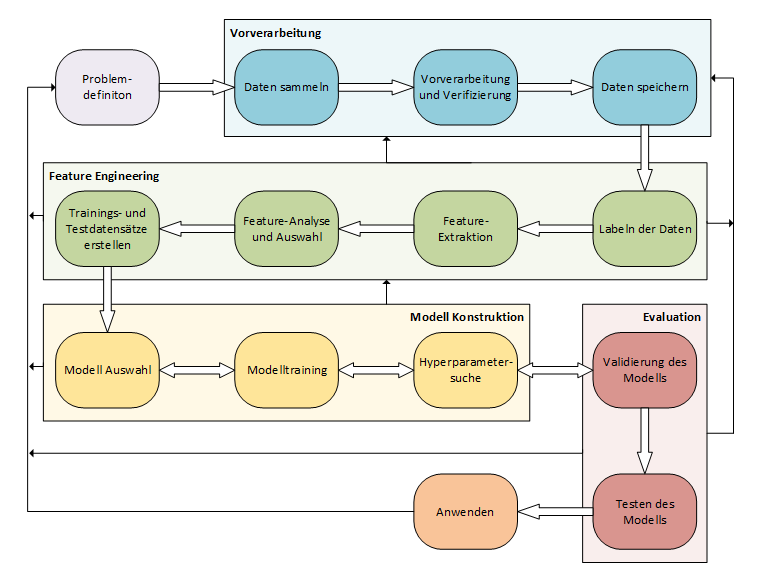
\includegraphics[width=\textwidth]{img/Grafiken/Machine Learning Workflow.png}
    \caption[Der Machine Learning Workflow]{Der \gls{Machine Learning Workflow} und seine Prozessschritte.}
    \label{fig:MLWorkflow}
\end{figure}


In der Grafik \ref{fig:MLWorkflow} sind Rückführungen zu früheren Prozessschritten zu sehen. Dadurch entstehen Schleifen. Einige dieser Schleifen sind optional und nur notwendig, wenn bspw. Testergebnisse sehr unbefriedigend sind. Ein Beispiel hierfür ist die Rückkehr zur Problemdefinition. Andere Schleifen sind übliche Praxis bei der Erstellung von Anwendung mit \glsdisp{ML}{maschinellem Lernen}. Z.B. ist die Suche von \gls{Hyperparameter} immer mit der Rückkehr zum Training verbunden \cite{Biswas.2022, Zheng.2018, Zheng.2015, Elshawi.2019}. 

\subsection{Problemdefinition und Vorverarbeitung}

\textbf{Problemdefinition}\par
Ziel des \gls{Machine Learning Workflow}[s] ist es, eine Anwendung zu erstellen, welche ein spezifisches Problem löst. Das die klare Definition einer Aufgabe, ein elementarer Schritt ist von Algorithmen des \glsdisp{ML}{maschinellen Lernens}, ist in \autoref{sec:Grundlagen ML} verdeutlicht. Die klare Definition ist auch hilfreich für den Erwerb von Fachwissen im Bereich der Aufgabe. Dies kann für den weiteren verlauf des Workflows nützlich sein \cite{Biswas.2022, Zheng.2018, Nielsen.2020}. \dubpar

\textbf{Sammeln von Daten} \label{sec:Worflow DatSam}\par
Ein Modell benötigt Daten für das Training. In diesem Schritt geht es darum, Rohdaten zu sammeln, die relevant sind für die Aufgabe, um diese weiterzuverarbeiten. Je nach Aufgabe ist dieser Prozess unterschiedlich aufwendig \cite{Biswas.2022, Elshawi.2019}. \dubpar

\textbf{Vorverarbeitung der Daten}\par
Die gesammelten Rohdaten können uneinheitlich sein. Sollen bspw. Daten aus mehreren Abteilungen einer Firma verwendet werden, um ein Modell zu erstellen, kann es sein, dass Abteilung \(A\) ein anderes Datumsformat benutze als Abteilung \(B\). Auch können Lücken in Daten vorhanden sein. Solche Probleme sind zu filtern und zu bereinigen \cite{Biswas.2022, Elshawi.2019}. Ebenfalls kann es sinnvoll sein, hier eine Verifikation der Daten vorzunehmen, um sicherzustellen, dass die Rohdaten auch die erwartete Information beinhalten \cite{Shearer.2000}. \dubpar

\textbf{Speicherung der Daten}\par
Frühzeitige Überlegungen zur Speicherung der Rohdaten sind vorteilhaft für den weiteren Verlauf des \gls{Machine Learning Workflow}[s]. Je nach Projekt sind andere Datenformate besser geeignet als andere. Auch der Speicherort ist relevant. Solche Überlegungen sorgen für einen effizienteren Ablauf des \gls{Machine Learning Workflow}[s] \cite{Biswas.2022}. 

\subsection{Labeln der Daten}
Wenn eine \glsdisp{überwachtes Lernen}{überwachte Lernmethode} verwendet werden soll, dann wird ein \gls{Zielvektor} benötigt. Dieser ist i.d.R. manuell zu erstellen. Das kann je nach Datenmenge und Datenart unterschiedlich aufwendig sein \cite{Biswas.2022}. Ein Beispiel aus der Bildverarbeitung ist eine Anwendung, welche Ampeln erkennen soll. In diesem Prozessschritt müssen alle Bilder, die für das Training verwendet werden sollen, mit einem \gls{Label} \textit{Ampel} oder \textit{keine Ampel} versehen werden. 

\subsection{Extraktion und Konstruktion der Features} \label{sec:ML FeatExtr}
Aus den Rohdaten müssen \gls{Feature}[s] kreiert werden, mit denen das Modell lernen kann. Dazu sind Überlegungen anzustellen, welche \gls{Feature}[s] sich aus den Rohdaten extrahieren lassen. Hierbei ist Fachwissen über die Aufgabe und die Rohdaten von großem Vorteil. Dadurch ist es möglich die Nützlichkeit möglicher \gls{Feature}[s] zu beurteilen und auch selbst kreative \gls{Feature}[s] zu entwerfen. Fachwissen wird auch benötigt, um gezielten \gls{Bias} in das Modell einzuführen. Auch ungewollter \gls{Bias} ist mit Fachwissen in manchen Fällen identifizierbar (\autoref{sec:Herausforderungen ML}). Generell ist in diesem Prozessschritt viel Achtsamkeit in Bezug auf \gls{Bias} sinnvoll \cite{Zheng.2018, Geron.2019}. \par

Auch auf \gls{Leakage} ist zu achten. Ein Beispiel wie \gls{Leakage} entstehen kann, ist die Komprimierung von Zeitreihen zu \gls{Feature}[s] (\autoref{sec:sequenzen ML}). Aus der Zeitreihe \(A\) sind komprimierte  \gls{Feature}[s] zu extrahieren, genauso wie aus der Zeitreihe \(B\). Was nicht bemerkt wird ist, dass diese eine zeitliche Überlappung haben. Dadurch sind die komprimierten Datenpunkte zu \(A\) und \(B\) nicht unabhängig voneinander. Das kann dazu führen, dass die Proben im Datensatz zu wenig Varianz aufweisen und das Modell lernt nicht zu \glsdisp{Generalisierung}{generalisieren}. Auch für die Evaluation kann das zu Problemen führen \cite{Zheng.2018, Geron.2019}. \par

Extrahierte \gls{Feature}[s] lassen sich Transformieren. Solche Transformationen zielen meistens auf eine Veränderung der Verteilung ab. Dies kann Modellen helfen aus \gls{Feature}[s] besser zu lernen. \dubpar

\textbf{Gruppierung}\\
Die Werte in einem \gls{Feature} werden in Gruppen eingeteilt. Dies kann durch vom Ersteller gewählte Wertebereiche erfolgen, oder nach statistischen Prinzipien, wie nach Quantilen. Dabei werden die Werte in gleich große Gruppen aufgeteilt. Z.B. werden die Werte bei einer Einteilung nach Perzentile in 100 Gruppen eingeteilt und in jeder befindet sich die gleiche Anzahl an Werten. Die Gruppen sind durchnummeriert. Die Nummer der Gruppe ist das neue konstruierte \gls{Feature} \cite{Zheng.2018}. \dubpar

\textbf{Power Transformationen}\\
Power Transformationen zielen darauf ab, die Varianz innerhalb eines \gls{Feature}[s] zu stabilisieren. Ein Beispiel ist die logarithmische Transformation. \gls{Feature}[werte] die sich über mehrere Größenordnungen verteilen, besitzen eine sehr hohe Varianz. Die Anwendung eines Logarithmus auf diese Verteilung komprimiert den Wertebereich. Dies reduziert die Varianz und erhöht die Vergleichbarkeit der Daten. Die Abbildung \ref{fig:bspLogTrans} veranschaulicht die logarithmische Transformation \cite{Zheng.2018}. 

\begin{figure}[htb]
    \centering
    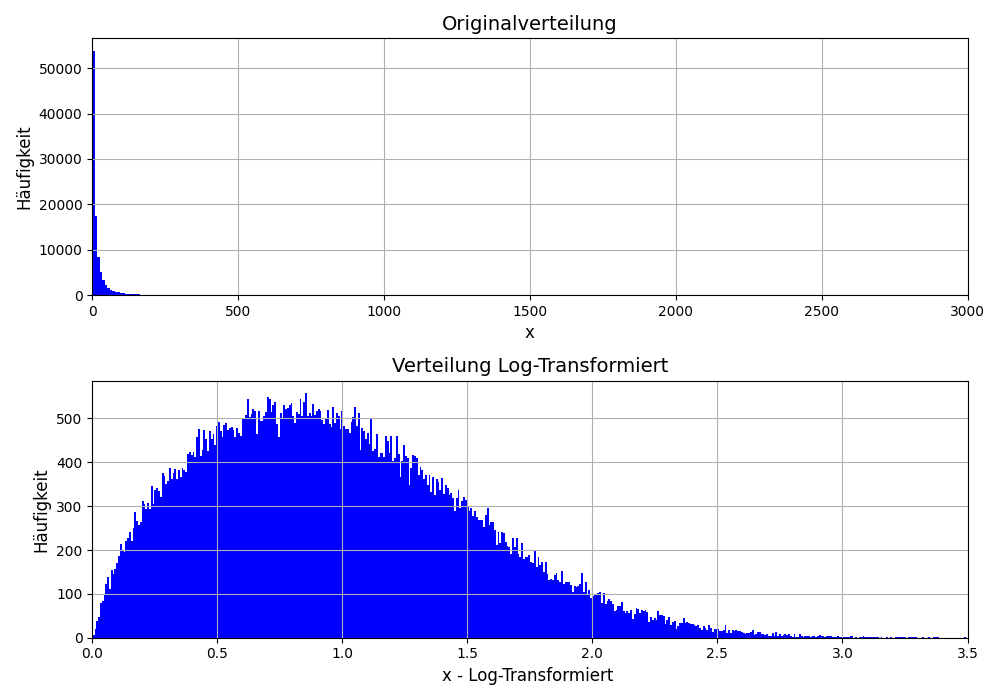
\includegraphics[width=0.9\textwidth]{img/Plots/Log-Transfomation.png}
    \caption[Beispielanwendung der logarithmischen Transformation.]{Beispielanwendung der logarithmischen Transformation. Werte eines \gls{Feature}[s], welche sich über mehrere Größenordnungen verteilen. Die Anwendung des Logarithmus verkleinert den Wertebereich erheblich.}
    \label{fig:bspLogTrans}
\end{figure}

Eine weitere Power Transformation ist die Box-Cox-Transformation. Diese versucht eine Verteilung näher an eine Normalverteilung zu bringen. Dies kann hilfreich sein, da einige Modelle besser mit Normalverteilung umgehen können. Die Formel \ref{eq:BoxCox} zeigt die Rechenvorschrift der Box-Cox-Transformation.

\begin{equation}
    \label{eq:BoxCox}
    x(\lambda) = 
    \begin{cases} 
    \frac{x^\lambda - 1}{\lambda} & \text{if } \lambda \neq 0, \\
    \ln(x) & \text{if } \lambda = 0.
    \end{cases}
\end{equation}

Der Parameter \(\lambda\) ist über eine Optimierung zu ermitteln, sodass die resultierende Verteilung möglichst nah einer Normalverteilung ist. Die Abbildung \ref{fig:bspBoxCox} zeigt die Auswirkung der Box-Cox-Transformation auf ein \gls{Feature} \cite{Zheng.2018}. 

\begin{figure}[htb]
    \centering
    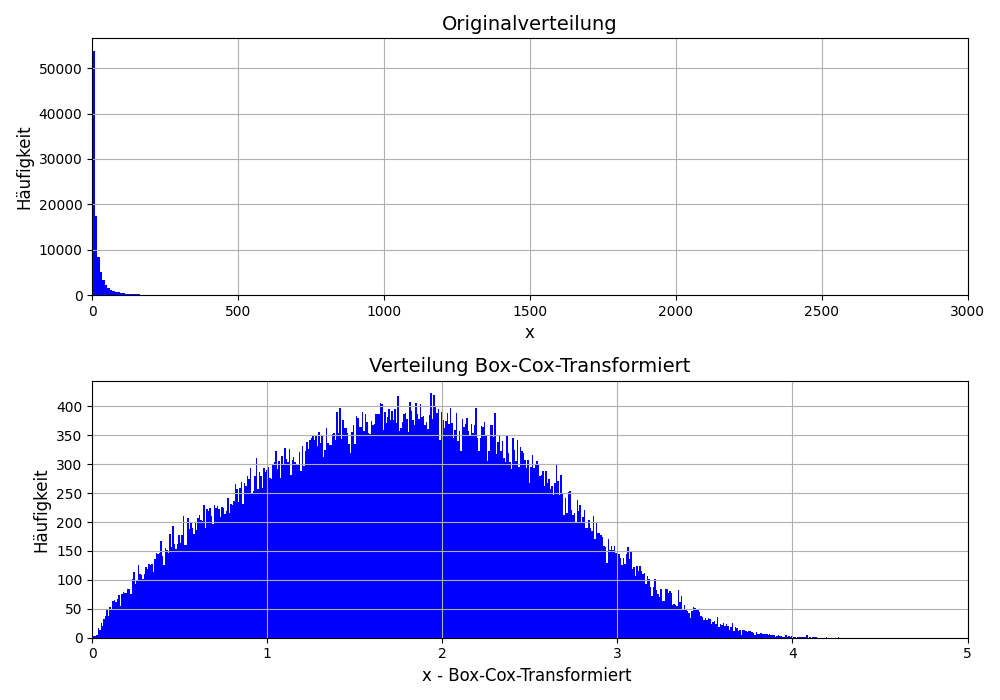
\includegraphics[width=0.9\textwidth]{img/Plots/Box-Cox-Transfomation.png}
    \caption[Beispielanwendung der Box-Cox-Transformation.]{Beispielanwendung der Box-Cox-Transformation. Werte eines \gls{Feature}[s], welche sich nicht normal verteilen. Die Anwendung verkleinert den Wertebereich erheblich und nähert die Verteilung einer Normalverteilung an.}
    \label{fig:bspBoxCox}
\end{figure}

Auch können aus bestehenden \gls{Feature}[s] neue kreiert werden. Ein Beispiel hierfür sind Interaktionsfeatures. Die einfachste Form ist die paarweise Multiplikation von \gls{Feature}[s]. Dies ist interpretierbar als eine Verknüpfung mit einem logischen UND. Dadurch entstehen neue \gls{Feature}[s] für das Modell, welche die Information von \gls{Feature}[s] enthalten, welche gerade in Kombination miteinander nützlich sind. Gerade einfachere Modelle, die eigenständig nicht so gut darin sind komplexe Zusammenhänge zu erkennen, können von dieser kombinierten Information profitieren \cite{Zheng.2018}.\par

Wird mit Sequenzen gearbeitet, dann findet in dem Prozessschritt der \gls{Feature}-Extraktion und Konstruktion ebenfalls die Konstruktion von \gls{Feature}[s] statt, welche versuchen, die Information der Sequenz zu komprimieren (\autoref{sec:sequenzen ML}) \cite{Nielsen.2020}. 

\subsection{Feature Analyse und Auswahl} \label{sec:ML FeatSelect}
Aus der Menge der \gls{Feature}[s] sind diejenigen auszuwählen, welche dem Modell übergeben werden sollen. Eine sorgfältige Auswahl der \gls{Feature}[s] ist wichtig, um ein zuverlässiges Modell zu erstellen. Hauptziel ist es, die \gls{Feature}[s] auszuwählen, mit welchen die Performance des Modells maximal wird. Ein weiteres Ziel ist die Minimierung der \gls{Feature}[anzahl], um den Rechenaufwand zu reduzieren. Eine kleinere Anzahl an \gls{Feature}[s] macht das Modell effizienter \cite{Kuhn.2013, Guyon.2003}. Wie in \autoref{sec:Herausforderungen ML} beschrieben, können \gls{Feature}[s], welche keine Information zur Erfüllung der Aufgabe besitzen, \gls{Underfitting} verursachen. Ebenfalls sind die \gls{Feature}[s] auf ungewollten \gls{Bias} zu überprüfen. Die Identifikation von ungewollten \gls{Bias} ist nicht einfach. Fachwissen und Wissen über typische Quellen von \gls{Bias} können dabei helfen \cite{Mehrabi.2019, Nielsen.2020}. In der Praxis wird zwischen drei Methoden für die Selektion von \gls{Feature}[s] unterschieden \cite{Guyon.2003}. \dubpar

\textbf{\gls{Filter Methoden}}\par
\gls{Filter Methoden} bewerten \gls{Feature}[s] Modell unabhängig und univariat. Das bedeutet, sie bewerten jedes \gls{Feature}[s] für sich. Mögliche Informationen, die durch die Kombination mehrerer \gls{Feature}[s] entstehen, werden nicht berücksichtigt. Sie vergeben für jedes \gls{Feature} eine Wertung, wodurch eine Rangfolge entsteht. Durch die univariate Bewertung können auch redundante \gls{Feature}[s] in die Auswahl aufgenommen werden, wenn sie individuell einen hohen Wert erzielen. Es gibt \gls{Filter Methoden} die auf Regressionsprobleme ausgelegt sind und Methoden, die auf \gls{Klassifikation}[sprobleme] ausgelegt sind. Da für diese Arbeit die Methoden für \gls{Klassifikation}[sprobleme] relevant sind, werden nur diese hier vorgestellt.\par

\textit{Gegenseitige Information:} Die gegenseitige Information stammt aus der Informationstheorie und ist ein Maß für die Abhängigkeit zweier Variablen. In diesem Fall zwischen den Klassen \(Y\) und einem \gls{Feature} \(X\). Die Aussage der gegenseitige Information ist, wie viel Information eine Variable über eine Andere hat. Die Formel \ref{eq:MutInfo} zeigt die Berechnung. 

\begin{equation}
I(X; Y) = \sum_{y \in Y} \sum_{x \in X} P_{X,Y}(x, y) \log \left( \frac{P_{X,Y}(x, y)}{P_X(x) P_Y(y)} \right)
\label{eq:MutInfo}
\end{equation}

Sind die Variablen unabhängig, gilt \(P(X)P(Y) = P(X,Y)\) und die gegenseitige Information ist gleich null. Besteht Abhängigkeit zwischen den Variablen ist \(I(X; Y) > 0\). Je höher die Abhängigkeit, desto größer ist \(I(X; Y)\) \cite{Cover.2006}.\par

\textit{Varianzanalyse:} Die Varianzanalyse ist eine statistische Methode. Sie überprüft, ob signifikante Unterschiede zwischen den Mittelwerten der Klassen liegen, in Bezug auf ein \gls{Feature}. Die Formeln \ref{eq:ANOVAVarZwiKla}, \ref{eq:ANOVAVarInKla} und  \ref{eq:ANOVA} zeigen die Berechnung.

\begin{equation}
Varianz\_zwischen\_den\_Klassen = \frac{\sum_{i=1}^{n} n_i(\bar{K}_i - \bar{K})^2}{(S - 1)}
\label{eq:ANOVAVarZwiKla}
\end{equation}

\begin{equation}
Varianz\_innerhalb\_der\_Klassen = \frac{\sum_{i=1}^{S} \sum_{p=1}^{n_i} (K_{ip} - \bar{K}_i)^2}{(N - S)}
\label{eq:ANOVAVarInKla}
\end{equation}

\begin{equation}
F\text{\_value} = \frac{Varianz\_zwischen\_den\_Klassen}{Varianz\_innerhalb\_der\_Klassen}
\label{eq:ANOVA}
\end{equation}

\(N\) ist die gesamte Anzahl der Proben. \(S\) ist die Anzahl an Klassen. \(n_i\) ist die Anzahl der Proben in der Klasse \(i\). \(\bar{K}_i\) ist der Mittelwert der Klasse \(i\) und \(\bar{K}\) ist der Mittelwert aller Proben. \(\bar{K}_{ip}\) ist das Element \(p\) in Klasse \(i\) \cite{Pathan.2022}. \par

Existiert keine Varianz innerhalb der Klassen, ist die Wertung null. Eine hohe Varianz in den Gruppen reduziert die Wertung und eine hohe Varianz zwischen den Gruppen erhöht die Wertung. Interpretierbar ist dies wie folgt: Umso besser sich die Klassen voneinander trennen lassen, desto besser ist die Wertung \cite{Pathan.2022, Guyon.2003}. \dubpar

\textbf{\gls{Wrapper Methoden}}\par

Anders als die \gls{Filter Methoden} treffen \gls{Wrapper Methoden} ihre Auswahl nicht univariat und auch nicht Modell unabhängig. Dadurch sind sie in der Lage, informative Kombinationen von \gls{Feature}[s] zu erkennen. Es kann auch sein, dass manche Modelle mit bestimmten \gls{Feature}[s] besser umgehen können als andere. Auch solche Einflüsse sind mit \gls{Wrapper Methoden} erkennbar \cite{Kuhn.2013, Guyon.2003}. \par

Die \gls{Wrapper Methoden} betrachten ein Modell als Blackbox. Sie entscheiden über die Eingabe in die Blackbox und beurteilen die Ausgabe von dieser. Die Ausgabe ist die Wertung einer Performancemetrik. Auf Performancemetriken wird später genauer eingegangen. Aus der Menge an \gls{Feature}[s] wird eins entnommen. Damit wird das Modell trainiert und die Performance bewertet. Wirkt sich das \gls{Feature} positiv auf die Metrik aus, dann wird es in die Auswahl aufgenommen. Wenn nicht, dann wird es zurückgelegt. Anschließend wird ein weiteres \gls{Feature} aus der Menge entnommen und in Kombination mit der bestehenden Auswahl überprüft. Wieder wird ein Modell trainiert und Performance bewertet. Dieser Prozess wird wiederholt, bis ein Abbruchkriterium erreicht ist. Dieses kann sich entweder auf die Performancemetrik beziehen, oder auf die \gls{Feature}[anzahl]. Z.B. kann das Vorgehen abgebrochen werden, wenn sich die Performance nicht mehr weiter verbessert, oder wenn eine gewünschte \gls{Feature}[anzahl] erreicht ist. Die Abbildung \ref{fig:WrapMeth} veranschaulicht das Vorgehen der \gls{Wrapper Methoden} \cite{Kuhn.2013, Guyon.2003}.

\begin{figure}[htb]
    \centering
    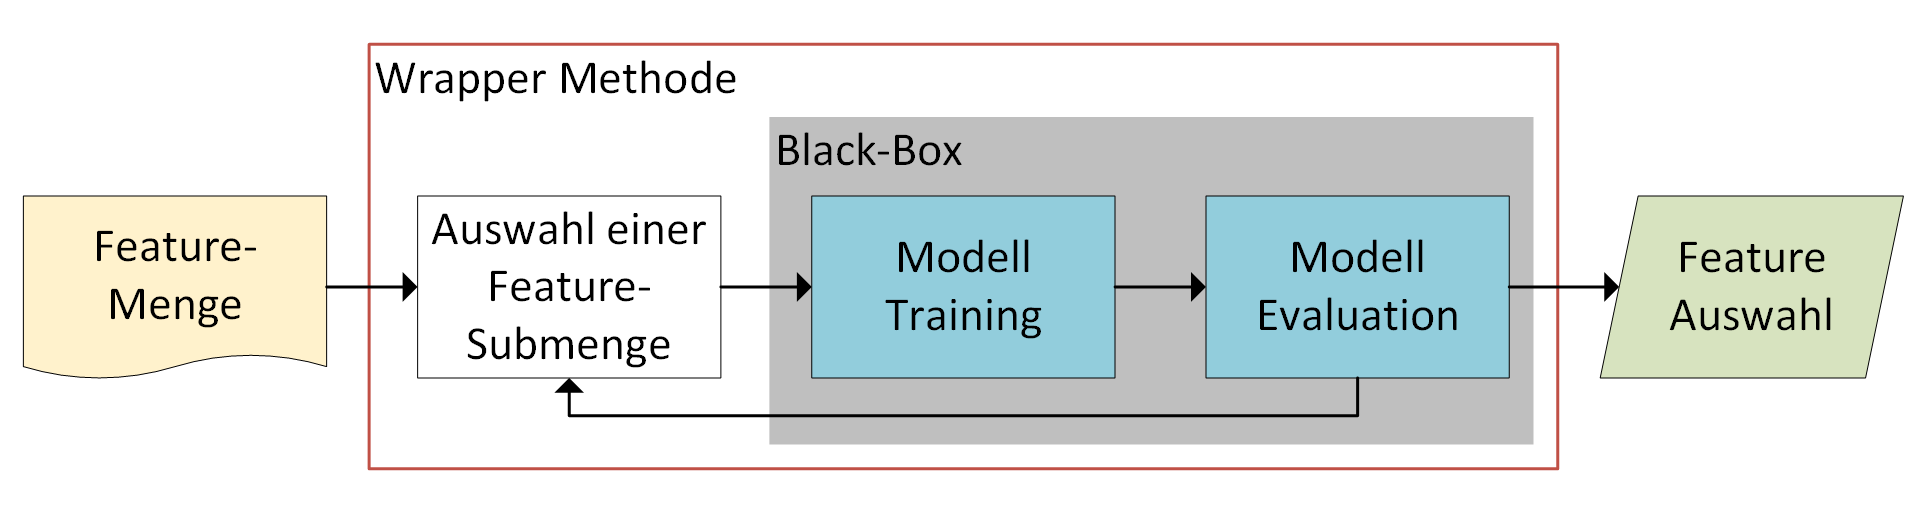
\includegraphics[width=0.9\textwidth]{img/Grafiken/Wrapper Methode bsp.png}
    \caption[Vorgehen der Wrapper Methoden.]{Vorgehen der \gls{Wrapper Methoden}. Aus der \gls{Feature}[menge] werden iterativ \gls{Feature}[s] ausgewählt und in Kombination mit der bestehenden \gls{Feature}[auswahl] evaluiert. Dazu wird das Modell in der Blackbox trainiert und die Performance bewertet.}
    \label{fig:WrapMeth}
\end{figure}

Bei den \gls{Wrapper Methoden} wird zwischen zwei Verfahren unterschieden. Der Vorwärtssuche und der Rückwärtssuche. Die Beschreibung von eben ist die der Vorwärtssuche. Bei der Rückwärtssuche befinden sich zu Beginn alle \gls{Feature}[s] in der Auswahl. Iterativ werden \gls{Feature}[s] aus der Auswahl ausgeschlossen. Dies geschieht, indem überprüft wird, wie sich der Verzicht auf ein \gls{Feature} auf die Performance auswirkt. Wirkt sich der Verzicht positiv aus, oder zumindest nicht negativ, dann wird das \gls{Feature} ausgeschlossen. Dieses Vorgehen, hat den Vorteil, dass Informationen, die in der Kombination von \gls{Feature}[s] liegen auf jeden Fall erkannt werden, da von Beginn an alle \gls{Feature}[s] zusammen bewertet werden. \dubpar

\textbf{\gls{Embedded Methoden}}\par

 \gls{Embedded Methoden} beurteilen \gls{Feature}[s], wie die \gls{Wrapper Methoden}, multivariat. Diese Auswahlmethoden sind direkt in bestimmten Modellen implementiert. Dadurch sind sie auch sehr abhängig vom Modell. Bei der linearen Regression können bspw. die Gewichte der \gls{Feature}[s] als ein Indikator für die Wichtigkeit der \gls{Feature}[s] sein. Andere Modelle implementieren diese Verfahren jedoch deutlich aussagekräftiger. Steht bereits fest, welches Modell verwendet werden soll, kann es sinnvoll sein \gls{Embedded Methoden} für die \gls{Feature}[selektion] zu verwenden, da sie eine Auswahl treffen, die sehr auf das Modell zugeschnitten ist. Steht das Modell noch nicht fest, können \gls{Feature}[s] ausgewählt werden, welche mit anderen Modellen weniger gut funktionieren \cite{Guyon.2003, Zheng.2018}.

 \subsection{Datensätze im maschinellen Lernen} \label{sec:Datensätze ML}
 Das Ergebnis der Feature-Extraktion, Konstruktion und Auswahl ist ein fertiger Datensatz, mit dem das Modell zu erstellen ist. Die Qualität und die Quantität der Daten hat dabei einen großen Einfluss auf die Performance des Modells (\autoref{sec:Herausforderungen ML}). Ziel ist es ein Modell zu entwerfen, was gut darin ist, unbekannte Proben zu schätzen. Um diese Fähigkeit zu beurteilen, werden einige Daten aus dem Datensatz zurückgehalten. Diese Daten werden nicht für das Training verwendet. Sie bleiben dem Modell unbekannt, um später die Performance auf unbekannten Daten zu beurteilen. Der Datensatz wird aufgeteilt in einen \gls{Trainingsdatensatz} und eine \gls{Testdatensatz}. Oftmals wird ein weiterer Datensatz mit Daten benötigt, die nicht für das Training verwendet werden. Dieser wird als Validierungsdatensatz bezeichnet. Der Validierungsdatensatz wird verwendet, um den Algorithmus auszuwählen und die \gls{Hyperparameter} einzustellen. Der Testdatensatz wird für den finalen Test verwendet, bevor das Modell angewendet wird \cite{Burkov.2019}. \par

 Für die Aufteilung der Daten auf die drei Datensätze gibt es keine allgemeingültige Regel. Eine gute Daumen-Regel ist 70 \% Trainingsdaten, 15 \% Validierungsdaten und 15 \% Testdaten. Es gibt Validierungsmethoden, durch die kein Validierungsdatensatz notwendig ist. Dies ist besonders praktisch, wenn die Datenmenge klein ist. Dadurch stehen mehr Daten für das Training zur Verfügung \cite{Burkov.2019}. Darauf wird später näher eingegangen. \par

 Bei Mehrklassen Klassifikation ist darauf zu achten, dass die Anzahl der Proben aus jeder Klasse ungefähr ist. Ist das nicht der Fall, handelt es sich um einen unbalancierten Datensatz. Dies kann problematisch sein, wie in \autoref{sec:Herausforderungen ML} in Bezug zu \gls{Bias} erläutert. Der Datensatz sollte balanciert werden. Eine Möglichkeit einen unbalancierten Datensatz auszubalancieren ist Undersampling. Dabei werden zufällig Proben aus den Mehrheitsklassen entfernt, bis alle Klassen ungefähr die gleiche Anzahl von Proben besitzen \cite{Burkov.2019}.


 \subsection{Auswahl des Algorithmus} \label{sec:ML ModellSelect}
 Die Auswahl des richtigen Algorithmus ist oftmals nicht einfach. Ist ausreichend Zeit, dann ist es sinnvoll mehrere Algorithmen auszuprobieren, um zu prüfen, welcher die beste Performance erzielt. Ebenfalls kann es hilfreich sein, die Auswahl anhand Kriterien einzuschränken. Die Auswahl der Kriterien geschieht anhand der Anforderungen und Randbedingung, die zum Zeitpunkt der Modellauswahl bekannt sind. Beispiele für solche Kriterien sind

 \begin{itemize}
     \item Die zur Verfügung stehende Rechenleistung.
     \item Die Geschwindigkeit der Schätzung
     \item Die zur Verfügung stehende Datenmenge
     \item Die Nachvollziehbarkeit des Schätzungsergebnisses
 \end{itemize}

 Um von den Modellen eins zu wählen, sind diese jeweils zu trainieren, einzustellen und zu validieren. Da die Einstellung der \gls{Hyperparameter} aufwendig seien kann, ist hier meistens eine grobe Einstellung ausreichend \cite{Burkov.2019, Geron.2019}.

\subsection{Überblick über Algorithmen und Modelle des maschinellen Lernens} \label{sec:ML Algorithmen}
Es existieren eine Vielzahl von Algorithmen und Modelle für \gls{ML}. Einen breiten Überblick über unterschiedliche Ansätze zu schaffen übersteigt den Rahmen dieser Arbeit. Aus diesem Grund werden hier die Funktionsprinzipien einer Auswahl von Modellen vorgestellt, die für diese Arbeit relevant sind. 

\textbf{k-Means Algorithmus} \par
k-Means ist ein Algorithmus der Clusteranalyse. Es ist eine \glsdisp{unüberwachtes Lernen}{unüberwachte Lernmethode}. Bei diesem ist der \gls{Hyperparameter} \(K\) auf die Anzahl der Klassen einzustellen, die in den Daten gefunden werden sollen. Aus dem \gls{Trainingsdatensatz} werden \(K\) zufällige Datenpunkte als Clusterzentren initialisiert. Iterativ werden nun neue Datenpunkte aus dem \gls{Trainingsdatensatz} gezogen. Die Distanz zwischen den Datenpunkten und den Clusterzentren wird ermittelt. Der Datenpunkt wird dem Cluster zugeordnet, zu dessen Zentrum die kleinste Distanz besteht. Anschließend findet eine Aktualisierung der Clusterzentren statt, indem die Mittelpunkte der Cluster berechnet werden. Die Mittelpunkte sind die neuen Zentren für die nächste Iteration \cite{Burkov.2019, Goodfellow.2016, Duda.2001}. \dubpar


\textbf{Hierarchisches Clustering} \par
Hierarchisches Clustering umfasst ebenfalls Algorithmen der Clusteranalyse. Es sind \glsdisp{unüberwachtes Lernen}{unüberwachte Lernmethoden}. Anders als bei k-Means ist keine \gls{Hyperparameter}[einstellung] der Clusteranzahl notwendig. Ansatz von hierarchischen Clustering Methoden ist, dass sich viele Cluster in Subcluster unterteilen lassen, welche sich ebenfalls in Subcluster unterteilen lassen. Als Beispiel wird ein Cluster \textit{Tiere} genommen. Dieses kann unterteilt werden in \textit{Säugetiere} und \textit{Reptilien}. Das Cluster \textit{Säugetiere} ist weiter unterteilbar in \textit{Fleischfresser} und \textit{Pflanzenfresser}. Hierarchisches Clustering versucht solche hierarchischen Strukturen zu modellieren. Dazu gibt es zwei Verfahren: agglomeratives  Clustering und divisives Clustering. Beim agglomerativen Clustering startet jeder Datenpunkt als eigenes Cluster. Bei jeder Iteration werden die beiden Cluster, die am nächsten zueinander liegen, zu einem Cluster zusammengefasst. Dadurch entsteht eine Baumstruktur. Der Anwender kann entscheiden, welche hierarchische Ebene die Aufgabe am besten modelliert und kann die Struktur an dieser Stelle auftrennen. Das diversive Clustering funktioniert genau andersherum. Alle Daten starten in einem großen Cluster. Die Subcluster, welche sich am unähnlichsten sind, werden in der nächsten Stufe aufgeteilt \cite{Duda.2001}. Die Abbildung \ref{fig:HiraClust} zeigt die beim hierarchischen Clustering entstehende Baumstruktur beispielhaft. 

\begin{figure}[htb]
    \centering
    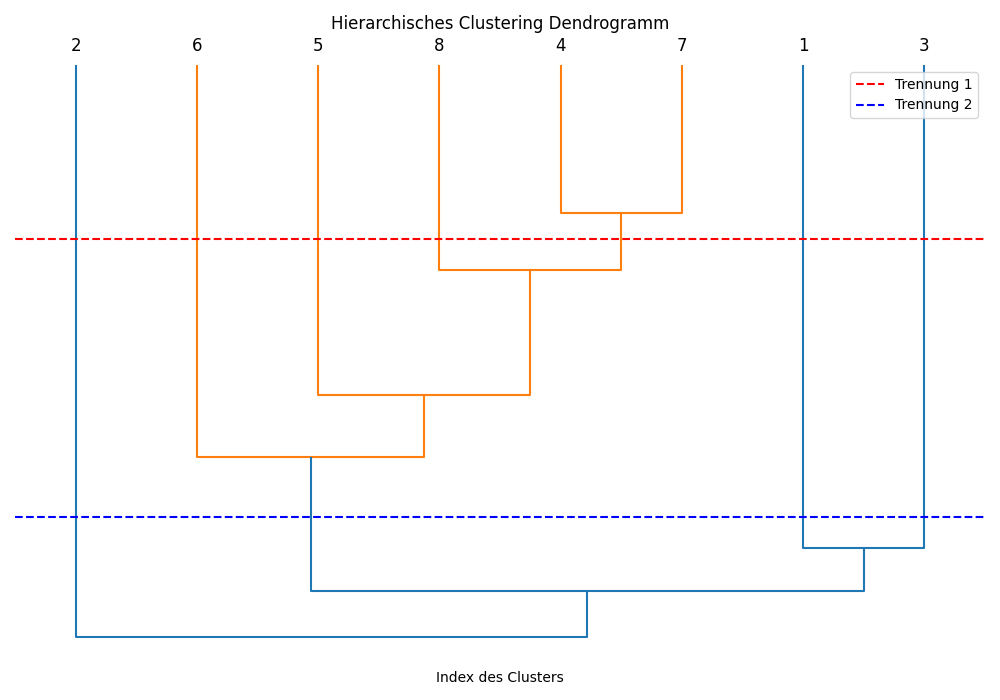
\includegraphics[width=0.9\textwidth]{img/Plots/Dendogramm Hierachisches Clustering.png}
    \caption[Dendrogramm zu einem Beispiel des Hierarchisches Clusterings.]{Dendrogramm zu einem Beispiel des Hierarchisches Clusterings. Die horizontalen Linien zeigen, dass über die Cluster-Anzahl entschieden werden kann, durch die Wahl der Trennebene.}
    \label{fig:HiraClust}
\end{figure}

\dubpar
\textbf{Logistische Regression} \par
\begin{wrapfigure}{l}{0.4\textwidth}
    \begin{center}
        \vspace*{-7mm}
        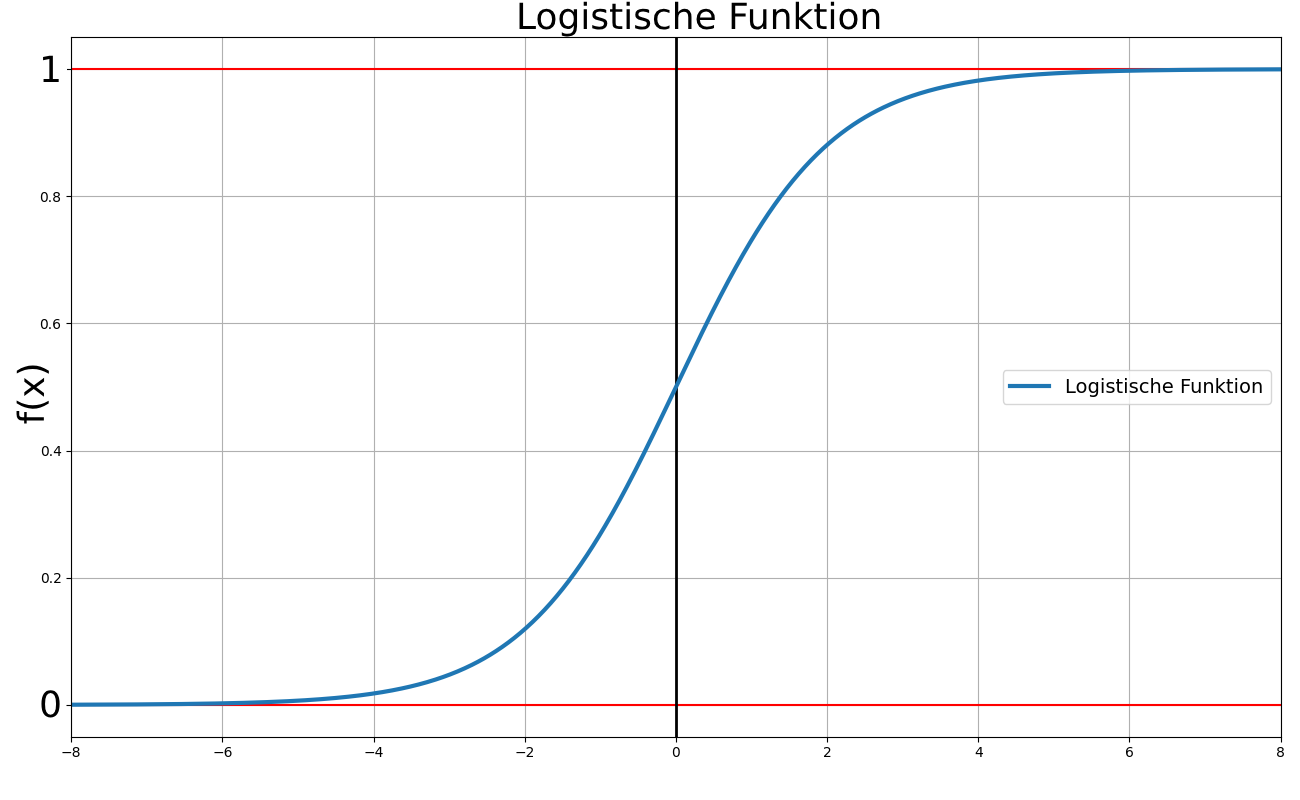
\includegraphics[width=0.4\textwidth, height=4cm]{img/Plots/Logistische Funktion.png}
        \vspace*{-10.5mm}
        \caption[Verlauf der logistischen Funktion.]{Verlauf der logistischen Funktion.}
        \label{fig:LogiFunc}
    \end{center}
\end{wrapfigure}
Die logistische Regression ist ein \gls{Klassifikation}[salgorithmus], auch wenn der Name anderes vermuten lässt. Es handelt sich um einen \glsdisp{überwachtes Lernen}{überwachten Algorithmus} für binäre \gls{Klassifikation} (\autoref{sec:ML klass und Reg}). Die logistische Regression verwendet die logistische Funktion aus der \autoref{eq:LogiFunc} (einen Spezialfall der Sigmoidfunktion), um Daten binär \((0,1)\) zuzuordnen. Die Abbildung \ref{fig:LogiFunc} zeigt den Verlauf der logistischen Funktion \cite{Burkov.2019}. 

\begin{equation}
f(x) = \frac{1}{1 + e^{-x}}
\label{eq:LogiFunc}
\end{equation}

Die logistische Regression trägt das Wort \textit{Regression} im Namen, da es verwandt ist mit der linearen Regression. Die Modellformulierung ist so interpretierbar, dass ein lineares Regressionsmodell, auf einen Wertebereich von \((0,1)\) abgebildet wird. Die Modellformulierung ist in \autoref{eq:LogiReg} zu sehen.

\begin{equation}
\hat{y}_{\nomvec{w},b}(\nomvec{x}) = \frac{1}{1 + e^{-(\nomvecT{w}\nomvec{x})+\nomvec{b})}}
\label{eq:LogiReg}
\end{equation}

Wird eine Probe geschätzt und erhält einen Wert \(\hat{y}_{\nomvec{w},\nomvec{b}}(\nomvec{x}) > 0,5\) dann wird die Probe der Klasse \(1\) zugeordnet. Ist \(\hat{y}_{\nomvec{w},\nomvec{b}}(\nomvec{x}) < 0,5\), dann gehört die Probe in die Klasse \(0\) \cite{Burkov.2019, Goodfellow.2016}.

\dubpar
\textbf{Support Vector Machine (\acrshort{SVM})} \par
Eine \acrshort{SVM} ist ein Modell des \glsdisp{überwachtes Lernen}{überwachten Lernens} für binäre \gls{Klassifikation}. Es versucht die Datenpunkte im \gls{Feature}[raum] mittels einer Hyperebene zu separieren. Die Hyperebene wird als Entscheidungsgrenze bezeichnet. Die Punkte aus jeder Klasse, welche am nächsten zu der Entscheidungsgrenze liegen, werden als Support Vektoren bezeichnet. Mittels diesen wird die Entscheidungsgrenze so ausgerichtet, dass sie möglichst gleich weit entfernt von allen Support Vektoren verläuft. Im Trainingsprozess versucht die \acrshort{SVM} somit die maximale Abgrenzung zwischen den Klassen zu finden. Die Abbildung \ref{fig:bspLinSVM} veranschaulicht das Konzept der Entscheidungsgrenze und den Support Vektoren. 

\begin{figure}[htb]
    \centering
    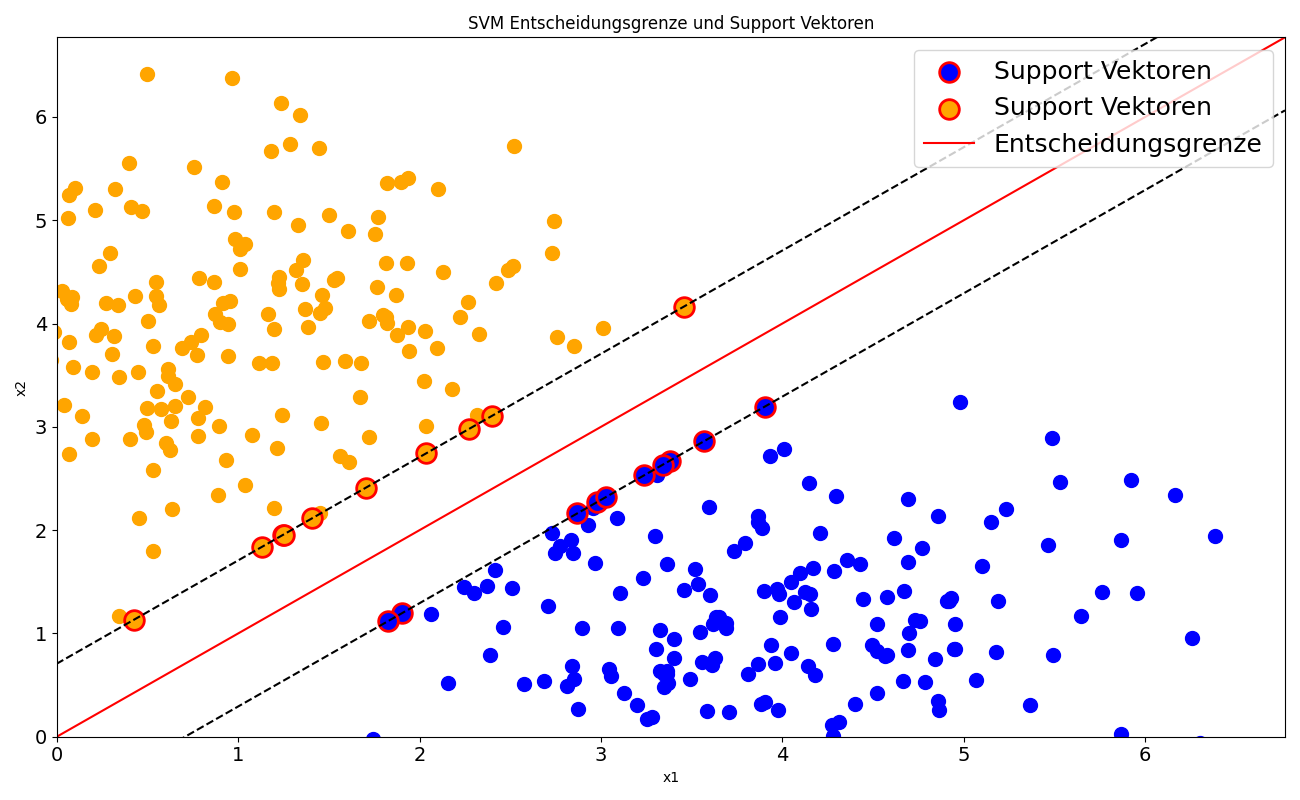
\includegraphics[width=0.9\textwidth]{img/Plots/SVM Beispiel.png}
    \caption[Beispiel der Funktionsweise einer SVM.]{Beispiel der Funktionsweise einer SVM. Anhand der Support Vektoren wird die Entscheidungsgrenze so ausgerichtet, dass sie gleich weit von beiden Klassen entfernt verläuft.}
    \label{fig:bspLinSVM}
\end{figure}

Definiert wird die Entscheidungsgrenze nach der Koordinatenform, wie die Gleichung \ref{eq:SVMdefHypEb} zeigt.

\begin{equation}
\nomvecT{w}\nomvec{x}+\nomvec{b}=0
\label{eq:SVMdefHypEb}
\end{equation}

Die Modellfunktion evaluiert die Klassenzugehörigkeit, indem sie überprüft, ob sich ein Datenpunkt oberhalb, oder unterhalb der Entscheidungsebene befindet. Dies erfolgt, indem der Datenpunkt in die Ebenengleichung eingesetzt wird. Anschließend gibt das Vorzeichen die Klassenzugehörigkeit an. Das ist in der Gleichung \ref{eq:SVMmodell} zu sehen. 

\begin{equation}
\hat{y}_{\nomvec{w},\nomvec{b}}(\nomvec{x}) = sgn(\nomvecT{w}\nomvec{x}+\nomvec{b}))
\label{eq:SVMmodell}
\end{equation}

Das Modell der Gleichung \ref{eq:SVMmodell} wird im Allgemeinen als lineare \acrshort{SVM} bezeichnet. Es gibt auch Verfahren, mit denen nicht-lineare Entscheidungsgrenzen verwendet werden können \cite{Burkov.2019, Goodfellow.2016, ShalevShwartz.2014}. \dubpar

\textbf{Random Forest}\par
Der Random Forest Algorithmus gehört zu den \glsdisp{überwachtes Lernen}{überwachten Lernverfahren} und ist eine Ensemble-Methode. Ensemble-Methoden nutzen ein Ensemble aus mehreren einfachen Modellen für ihre Entscheidungsfindung. Der Random Forest Algorithmus besteht aus mehreren Entscheidungsbäumen. Ein Entscheidungsbaum ist ein grafischer Ansatz für \gls{ML}. In einem Beispiel ist der Wert eines Autos zu schätzen. Ein Entscheidungsbaum betrachtet in den Knoten die \gls{Feature}[s] und entscheidet sich auf Basis von Schwellwerten, welcher Kante er folgt. Bezogen auf das Beispiel wird in einem Knoten überprüft, ob das Auto älter oder jünger als 10 Jahre ist. Beim Erreichen der Blätter des Baumes wird eine Entscheidung getroffen. Während des Trainings versucht ein Baum funktionierende Schwellwerte in den Knoten zu finden. Entscheidungsbäume eignen sich für die \gls{Klassifikation}, sowie die Regression. Auch Mehrklassenprobleme sind ohne weiteres mit Entscheidungsbäumen lösbar \cite{Burkov.2019, Bishop.2006, Goodfellow.2016}. \par

Der Random Forest Algorithmus zieht aus dem \gls{Trainingsdatensatz} eine zufällige Menge an Proben mit zurücklegen. Damit wird ein einzelner Baum trainiert. In den verschiedenen Knoten wird immer nur eine zufällige Teilmenge der \gls{Feature}[s] berücksichtigt. Durch diese Zufallsmechanismen wird gewährleistet, dass die resultierenden Bäume unterschiedlich sind. Das Modell schätzt eine unbekannte Probe, indem sie von allen Entscheidungsbäumen evaluiert wird. Das finale Ergebnis entsteht durch eine Mehrheitsentscheidung. Typische \gls{Hyperparameter} von  Random Forest Algorithmen sind die Anzahl der Bäume und die Baumtiefe \cite{Burkov.2019, Breiman.2001}. \dubpar

\textbf{Gradient Boosting} \par
Gradient Boosting gehört zu den \glsdisp{überwachtes Lernen}{überwachten Lernverfahren} und ist ebenfalls eine Ensemble-Methode, die auf Entscheidungsbäumen beruht. Während Random Forest seine Entscheidungsbäume unabhängig und parallel aufbaut, erstellt Gradient Boosting diese sequenziell. \par 

Zu Beginn wird ein konstanter Entscheidungsbaum initialisiert. Dieser ist die Ausgangssituation für die Modellierung mit Entscheidungsbäumen. Es existiert ein einziger Knoten, welcher auf jede Eingabe identisch bewertet. Mit diesem konstanten Entscheidungsbaum werden alle Proben im \gls{Trainingsdatensatz} bewertet. Anschließend wird die Abweichung gemessen. Diese Abweichung wird für den nächsten Entscheidungsbaum als \gls{Label} für die Daten verwendet. Der folgende Baum lernt somit die Fehler seines vorausgegangenen Baumes zu schätzen. Sequentiell lernen die folgenden Bäume den verbleibenden Fehler zu schätzen. \par

Ist eine unbekannte Probe zu schätzen, weiß das Modell nach dem Training, wie es die Fehler in den Bäumen korrigieren muss. Ein wichtiger \gls{Hyperparameter} im Gradient Boosting ist die Lernrate. Diese bestimmt die Stärker der Korrektur für jede Stufe in der Sequenz. Ist bspw. laut Entscheidungsbaum die Schätzung um den Wert \(a\) zu korrigieren, sorgt die Lernrate \(\alpha\) dafür, dass die Schätzung nur um \(\alpha \cdot a\) korrigiert wird. Dies kann Overfitting vermeiden \cite{Burkov.2019}. \par

Eine Variante des Gradient Boosting wird als histogrammbasiertes Gradient Boosting bezeichnet. Bei dieser werden die Features zuvor gruppiert, ähnlich der Gruppierung bei der Feature-Konstruktion (\autoref{sec:ML FeatExtr}). Dadurch wird die Anzahl unterschiedlicher Werte reduziert. Das Gradient Boosting ist somit effizienter durchzuführen \cite{Ke.2017}. 
\dubpar


\textbf{Long Short-Term Memory (\acrshort{LSTM})} \par
\acrshort{LSTM}[s] sind Modelle des \gls{Deep Learning}. Sie sind eine spezielle Form von rekurrenten neuronalen Netzwerken (\acrshort{RNN}[s]). \acrshort{RNN}[s] sind darauf ausgelegt Sequenzen verstehen zu können. Dies wird durch Rückführungen erreicht. Die Einheiten in den Schichten eines \acrshort{RNN}[s] besitzen einen Zustandsspeicher. Als Eingabe erhält eine Einheit die Ausgabe der vorherigen Schicht, und die Rückführung des eigenen Zustandsspeichers. Das Ergebnis aktualisiert den Zustandsspeicher. Somit wirken frühere Zeitschritte in den Daten auf spätere, wodurch Mustererkennung in Sequenzen möglich wird.\par

Es existieren jedoch einige Komplikationen klassische \acrshort{RNN}[s] anzuwenden. Aus diesem Grund haben sich sogenannte \textit{Gated \acrshort{RNN}[s]} für die Realisierung durchgesetzt. Ein solches \acrshort{RNN} ist das \acrshort{LSTM}. Die Kernidee von \acrshort{LSTM}[s] ist eine Regulierung des Zustandsspeichers der Einheiten. Der Zustandsspeicher wird durch drei Arten von Toren reguliert. Einem Eingangstor, einem Vergesstor und einem Ausgangstor. Diese Struktur ermöglicht es, Informationen über lange Zeiträume zu speichern, irrelevant gewordene Informationen zu vergessen und den Informationsfluss innerhalb der Zelle zu regulieren.

\begin{itemize}
    \item Das Eingangstor steuert, welche neuen Informationen zu einem Zeitpunkt in den Zustandsspeicher aufgenommen werden.
    \item  Das Vergesstor entscheidet, welche Teile des aktuellen Zustands erhalten bleiben oder verworfen werden.
    \item Das Ausgangstor bestimmt, welche Informationen aus dem Zustandsspeicher an den Ausgang weitergegeben werden.
\end{itemize}

Diese Mechanismen erlauben es \acrshort{LSTM}[s]s, sowohl kurzfristige als auch langfristige Datenabhängigkeiten zu lernen und effektiv zwischen relevanten und irrelevanten Informationen zu unterscheiden \cite{Burkov.2019, Goodfellow.2016}. \par

\textbf{Gated Recurrent Unit (\acrshort{GRU})}
Die \acrshort{GRU} lässt sich als vereinfachte Form eines \acrshort{LSTM}[s] betrachten. Sie verwendet ebenfalls Tore für die Handhabung langfristiger und kurzfristiger Abhängigkeiten in sequenziellen Daten. \acrshort{GRU}[s] vereinfachen die Struktur von \acrshort{LSTM}[s], indem sie nur zwei Tore verwenden. Ein Update-Tor und ein Reset-Tor. \par

\begin{itemize}
    \item Das Update-Tor entscheidet, inwieweit der aktuelle Zustandsspeicher durch den neuen Zustand ersetzt werden soll. Es ermöglicht die Dauer zu bestimmen, wie lange Information bewahrt wird.
    \item Das Reset-Tor ermöglicht es zu entscheiden, wie viel vom aktuelle Zustandsspeicher verwendet werden soll, um den neuen Zustand zu berechnen.
\end{itemize}

\acrshort{GRU}[s] sind einfacher zu trainieren als \acrshort{LSTM}[s] und sie können ähnlich gut in ihrer Performance sein \cite{Lazzeri.2021, Goodfellow.2016}. 



\subsection{Training und Validierung des Modells} \label{sec:ML Metriken, Valid}
Das Modell wird mit der \gls{Trainingsdatensatz} trainiert. Dieser Prozess ist modellabhängig. Die meisten \gls{Bibliothek}[en], die Algorithmen für \gls{ML} implementieren, haben automatische Routinen um die Modelle zu trainieren. Nach dem Training wird die Performance mit dem Validierungsdatensatz beurteilt \cite{Burkov.2019, Geron.2019, Zheng.2015}. Für die Performancebewertung existieren verschiedene Methoden. Hier werden zwei vorgestellt. \dubpar

\textbf{\gls{Accuracy}}\par

Die \gls{Accuracy} berechnet sich für ein \gls{Klassifikation} [sproblem] aus dem Verhältnis der Anzahl der richtig \glsdisp{Klassifikation}{klassifizierten} Proben \(TP\) und der Gesamtanzahl der Proben \(N\). Dies zeigt die Formel \ref{eq:MLaccuracy} \cite{Zheng.2015}.

\begin{equation}
Accuracy = \frac{|TP|}{|N|}
\label{eq:MLaccuracy}
\end{equation}

\textbf{\gls{Konfusionsmatrix}}\par
Eine \gls{Konfusionsmatrix} bietet Einblick in die Fehler, die das Modell macht. Sie zeigt, welche Verwechslungen stattfinden. In einem Beispiel wird die Performance eines Spam-Filters beurteilt. Dieser wurde mit 200 E-Mails validiert. Die Tabelle \ref{tab:bspConfMat} zeigt die \gls{Konfusionsmatrix} des Spam-Filters \cite{Zheng.2015}.

\begin{table}[h]
    \centering
    \begin{tabular}{|l|c|c|}
        \hline
                                    & Schätzung: \textit{Spam} & Schätzung: \textit{kein Spam}\\
        \hline
        Label: \textit{Spam}        & 80 & 15 \\
        \hline
        Label: \textit{kein Spam}   &  5 & 100\\
        \hline
    \end{tabular}
    \caption{\gls{Konfusionsmatrix} eines Spam-Filters. Der Filter wurde mit 200 Proben evaluiert. 80 E-Mails sind korrekt als \textit{Spam} erkannt worden und 100 korrekt als \textit{kein Spam}. 5 E-Mails wurden fälschlicherweise als \textit{Spam} geschätzt und 15 fälschlicherweise als \textit{kein Spam}.}
    \label{tab:bspConfMat}
\end{table}

Wie bereits in \autoref{sec:Datensätze ML} erwähnt, ist es möglich den Validierungsdatensatz einzusparen. Das ist mit dem Verfahren \gls{Cross-Validation} möglich. Dabei wird der \gls{Trainingsdatensatz} in \(K\) gleich große Teile aufgeteilt. Anschließend werden \(K\) Modelle trainiert, dabei wird immer ein anderes Teil des \gls{Trainingsdatensatz}[es] zurückgehalten und für die Validierung verwendet. Somit existieren \(K\) Beurteilungen der Performance. Die Gesamtperformance ist der Mittelwert. Das Modell wird anschließend mit dem vollständigen \gls{Trainingsdatensatz} trainiert. Die Abbildung \ref{fig:CrossVal} veranschaulicht die \gls{Cross-Validation}.

\begin{figure}[htb]
    \raggedright
    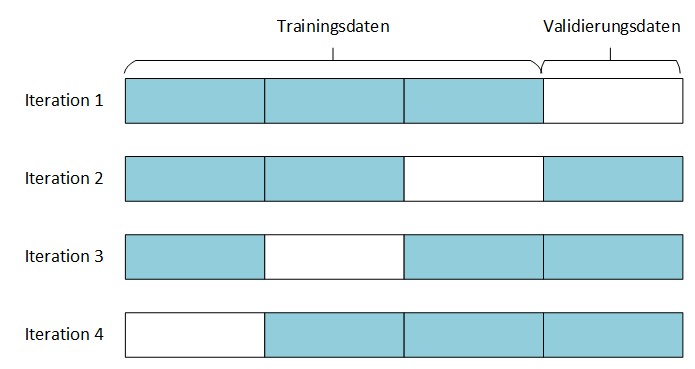
\includegraphics[width=0.9\textwidth]{img/Grafiken/Cross Validation.png}
    \caption[Verfahren der Cross-Validation.]{Verfahren der \gls{Cross-Validation}.  Der \gls{Trainingsdatensatz} wird in 4 Teile zerteilt, wovon jedes einmal als Validierungsdatensatz verwendet wird.}
    \label{fig:CrossVal}
\end{figure}

\subsection{Einstellung der Hyperparameter} \label{sec:ML HyperPara}
\gls{Hyperparameter} ermöglichen es Einfluss auf den Trainingsprozess eines Modells zu nehmen. Sie sind vor dem Training vom Anwender einzustellen. Ein Beispiel ist ein \gls{Regularisierung}[stherm]. Die Einstellung der \gls{Hyperparameter} ist sehr aufgabenspezifisch. Es gibt keine allgemeine Regel für optimale \gls{Hyperparameter}. Es ist ein Optimierungsproblem, welches sich mittels Algorithmen lösen lässt. Ziel der Optimierung ist die Maximierung des Validierungsergebnisses \cite{Zheng.2015}.\dubpar


\textbf{Grid Search}\par

Für alle \gls{Hyperparameter} wird ein Raster angegeben, z.B. für den \gls{Regularisierung}[stherm] \(C = \{0,1,1,10,100,1000\}\). Für jede Kombination von Werten der \gls{Hyperparameter} wird ein Modell trainiert und validiert. Am Ende werden die \gls{Hyperparameter} eingestellt, mit denen die beste Performance erzielt wurde. Diese Methode kann sehr rechenaufwändig sein, da jegliche Kombinationen zu prüfen sind. Gerade bei sehr feinen Rastern kann das Vorgehen viel Zeit in Anspruch nehmen \cite{Zheng.2015}.\dubpar

\textbf{Random Search}\par

Beim Random Search Verfahren bekommen die \gls{Hyperparameter} eine Wahrscheinlichkeitsverteilung zugewiesen, aus welcher diese ihre Einstellungswerte ziehen. Es wird eine festgelegte Anzahl an Kombinationen getestet. Bei jeder Iteration werden neue Zufallswerte gezogen. Dadurch ist der Rechenaufwand deutlich leichter zu überschauen als bei der Grid Search. Mit Random Search sind ähnlich gute Ergebnisse zu erzielen, wie mit Grid Search \cite{Zheng.2015, Burkov.2019}.


\subsection{Testen und Anwenden des Modells}
Die finalen Prozessschritte im \gls{Machine Learning Workflow} sind das Testen mit dem \gls{Testdatensatz} und die Integration des Modells in die Anwendung. Für das Testen werden die gleichen Metriken verwendet wie bei der Validierung (\autoref{sec:ML Metriken, Valid}). Ist der finale Test zufriedenstellend, kann das Modell in die Anwendung integriert werden. Ist dies nicht der Fall, ist eine Rückkehr zu früheren Prozessschritten notwendig \cite{Zheng.2015, Burkov.2019}.


    %Methodik------------------------------------------------------------------------------
    \chapter{Methodenentwicklung}\label{chap:Methodenentwicklung}

\section{Entwicklung des Gesamtkonzepts} \label{sec:Meth gesamtkonzept}
Um ein Gesamtkonzept für das \gls{Modul} zur automatischen Verhaltensklassifikation zu entwerfen, sind einige grundlegende Aspekte zu betrachten. Zentral ist die Definition der Aufgabe, die mittels maschinellem Lernen gelöst werden soll. Diese ist aus den Anforderungen an das \gls{Modul} abzuleiten. Ebenfalls ist die Rohdatengrundlage zu betrachten, aus welcher sich die Erfahrung, in Form von Features extrahieren lässt. Über die Rohdatengrundlage ist der Moduleingang bestimmbar. In diesem Kapitel werden deshalb die Modulanforderungen betrachtet und die Rohdatengrundlage und Voraussetzungen. Anschließend wird die maschinelle Lernaufgabe definiert. Die Erkenntnisse fließen in einem Gesamtkonzept für das Modul zusammen. Bezogen auf den \gls{Machine Learning Workflow} (\autoref{sec:MLWF}), wird hier auf  die \textit{Problemdefinition} und die Vorbereitung für das \textit{Sammeln von Daten} beschrieben. \par


\subsection{Anforderungen an das Modul} \label{sec:Meth Anforderungen}

Aus den Zielsetzungen für die Modul-Entwicklung (\autoref{sec:Zielsetzung}) lassen sich Anforderungen ableiten. Da explizit maschinelles Lernen verwendet werden soll, grenzt dieses Ziel die Methodenauswahl ein. Durch diese Eingrenzung, ist abzuleiten, dass Features zu extrahieren sind und ein maschinelles Lernmodell benötigt wird. Da Verhalten erkannt werden soll, steht fest, dass das Modell ein \gls{Klassifikation}[sproblem] lösen muss. Das grenzt die Methodenauswahl weiter ein. \par

 Das Konzept soll modular sein. Es muss sich einfach in eine Datenverarbeitungskette integrieren lassen, um für übergeordnete Systeme nutzbar zu sein. Dafür muss es ebenfalls Verhalten automatisiert auswerten. Eine manuelle Steuerung ist nicht erwünscht. Die Verarbeitung soll nur einen Datenstrom als Eingang erhalten, aus vorausgegangenen Modulen in der Verarbeitungskette. Aus dem Ziel der Echtzeitfähigkeit ergeben sich Anforderungen an die Laufzeit. Diese muss so kurz sein, dass sich nach Eintreffen des Ergebnisses noch Einfluss auf das Verhalten nehmen lässt. Die Verarbeitungsdauer des Moduls muss somit möglichst kurz sein. \par

 Neben der Zielsetzung ist der Zeitrahmen ein einschränkender Faktor. Um eine erfolgreiche Entwicklung in der vorgegebenen Zeit zu gewährleisten, muss der Implementierungsaufwand von Modul und maschinellem Lernmodell realisierbar sein. In Bezug auf das Gesamtkonzept wirkt sich dieser Fakt primär auf die Feature-Extraktion, Konstruktion und die Modellauswahl aus. Modelle, die komplex zu implementieren sind, können dadurch ungeeignet sein. Das Gleiche gilt für besonders komplexe Features.



\subsection{Rohdatengrundlage und Voraussetzungen} \label{sec:Meth RohDat}
Die Rohdaten sind fundamental für den Aufbau von Anwendungen des \glsdisp{ML}{maschinellen} Lernens. Im \gls{Machine Learning Workflow} wird sich ab dem zweiten Prozessschritt mit ihnen auseinandergesetzt (\autoref{sec:Worflow DatSam}). Die frühe Position im Ablauf zeigt, dass sämtliche folgenden Prozesse auf den Rohdaten fußen. Eine frühzeitige Bestandsaufnahme der zur Verfügung stehenden Rohdaten kann einen erfolgreichen Verlauf des Workflows gewährleisten. \par

Im \acrshort{OptiLiMa} Projekt wurden Rohdaten aus einem Mastputenstall gesammelt. Dieser wurde mit zwölf Kameras ausgestattet, die jeweils einen anderen Stallbereich abdeckten. Positioniert wurden die Kameras so, dass sie das Stallgeschehen aus der Vogelperspektive aufzeichneten. Die Abbildung \ref{fig:KamerasImStall} stellt die Einteilung des Mastputenstalls in die mit Kameras abgedeckten Bereiche dar. Eingezeichnet ist der ungefähre Verlauf der Futterbahnen.

\begin{figure}[htb]
    \centering
    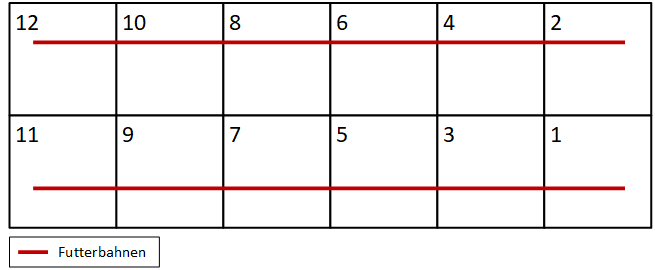
\includegraphics[width=0.9\textwidth]{img/Grafiken/Stallbereiche mit Futterbahn.png}
    \caption[Abteile des Mastputenstalls mit Verlauf der Futterbahnen.]{Abteile des Mastputenstalls mit Verlauf der Futterbahnen. Die Nummer in den oberen linken Ecken stehen für die IDs der Kameras.}
    \label{fig:KamerasImStall}
\end{figure}

Die Kameras nahmen einen Videostream auf. Die Bildinformationen wurden verwendet, um ein \gls{Detektion}[s]\glsdisp{Modul}{modul} anzuwenden. Dieses \glsdisp{Detektion}{detektierte} und \glsdisp{Lokalisation}{lokalisierte} die Puten im \gls{Frame}. Die \gls{Detektion} verlief in Echtzeit. Die \gls{Detektion}[en] wurde in einer Datenbank gespeichert, die sich auf einem Server befindet. Jeder Eintrag beinhaltet einen eindeutigen Zeitstempel und ein dazugehöriges \gls{Frame} in einem Videostream. Die Videostreams wurden auf Festplatten gespeichert. Insgesamt wurden  drei Mastdurchläufe aufgezeichnet. Ein Lebenszyklus der Puten umfasst ca. 4 Monate. Nach einer Aufzuchtphase von einem Monat kommen die Tiere in den Mastputenstall. Ab diesem Punkt begann die Datenerfassung. \par

Die Datensammlung im Mastputenstall war bereits vor Beginn dieser Arbeit abgeschlossen. Somit ließ sich kein Einfluss auf die Art und die Menge der zur Verfügung stehende Rohdaten nehmen. Die Videostreams liegen im mp4-Dateiformat vor. Das direkte Arbeiten auf der Datenbank mit den \gls{Detektion}[en] ist wegen des Datenvolumens und der Rechenleistung der Server nicht praktikabel. Aus diesem Grund wurde ein Tool entwickelt, das auf die Datenbank zugreift und Daten eines angegebenen Zeitintervalls herunterlädt. Die heruntergeladenen \gls{Detektion}[en] speichert das Tool in einer csv-Datei. In einer vorausgegangenen Arbeit im Rahmen des \acrshort{OptiLiMa} Projekts wurde ein \gls{Assoziation}[s]\glsdisp{Modul}{modul} entwickelt, das die \gls{Detektion}[en] nutzt. Somit steht ein \gls{MOT} System zur Verfügung. \par

Die \gls{Detektion} und die \gls{Assoziation} bauen auf dem Videostream auf. Jedes \gls{Frame} im Videostream hat einen eindeutigen Zeitstempel zugeordnet. Dadurch wird ersichtlich, dass die vorhandenen Rohdaten in Form von Zeitreihen vorliegen.

\subsection{Definition der Aufgabe} \label{sec:Meth DefAufgabe}
Ziel ist es, Verhaltensweisen der Mastputen zu klassifizieren (\autoref{sec:Zielsetzung}). Um eine Aufgabe zu formulieren, muss zunächst geklärt werden, was eine Verhaltensweise ist und wie sie sich erkennen lässt. In \cite{Levitis.2009} wird Tierverhalten definiert als Reaktionen von Individuen oder Gruppen auf Reize aus ihrer Umgebung. Das Suffix \textit{-weise} oder \textit{-art} bezeichnet eine Gewohnheit \cite{duden.art}. Eine Verhaltensweise ist somit ein Muster im Verhalten. Im Vorfeld dieser Arbeit wurden zwei Verhaltensweisen identifiziert, die besonders herausstechen. Diese werden hier als Kontrollgänge und Kämpfe bezeichnet. Im Folgenden werden diese beiden Verhaltensweisen erläutert. \dubpar

\begin{quote}

\textbf{Kontrollgänge}\par
Der Tierhalter unternimmt täglich Kontrollgänge im Maststall. Die Tiere reagieren auf den Tierhalter, wenn dieser den Stall betritt und umhergeht. Dabei finden Massenbewegungen statt. Die Tiere werden aufgeschreckt und fangen an, sich in Richtung des Tierhalters zu drängen. Oftmals beruhigen sich die Tiere noch während des Kontrollgangs. Nähert sich der Tierhalter ihrem Stallbereich, werden sie jedoch oftmals wieder aufgeschreckt und drängen sich erneut in seine Richtung. In seiner unmittelbaren Nähe weichen ihm die Tiere aus. Dadurch entsteht eine \gfuss{Traube} um den Tierhalter. Regelmäßig muss im Stall neues Stroh gestreut werden. Dafür fährt ein Traktor durch den Stall. Das Verhalten der Tiere ist in diesem Fall jedoch sehr ähnlich zum täglichen Kontrollgang. Die Tiere drängen zum Traktor. Um den Traktor bildet sich ein \gfuss{Traube}. Die \gfuss{Traube} ist dabei deutlich größer, aufgrund der Größe des Traktors. Fährt der Traktor durch den Stall, bleibt hinter ihm eine große freie Fläche zurück. Einige Puten nutzen diese Fläche, um dem Traktor nachzujagen. Teileweise füllt sich die Fläche jedoch nur gemächlich. Die Abbildung \ref{fig:bspKontrollg} zeigt einige Ausschnitte aus Kontrollgängen. 
\end{quote}


\begin{figure}[htb]
     \centering
     \begin{subfigure}[b]{0.4\textwidth}
         \centering
         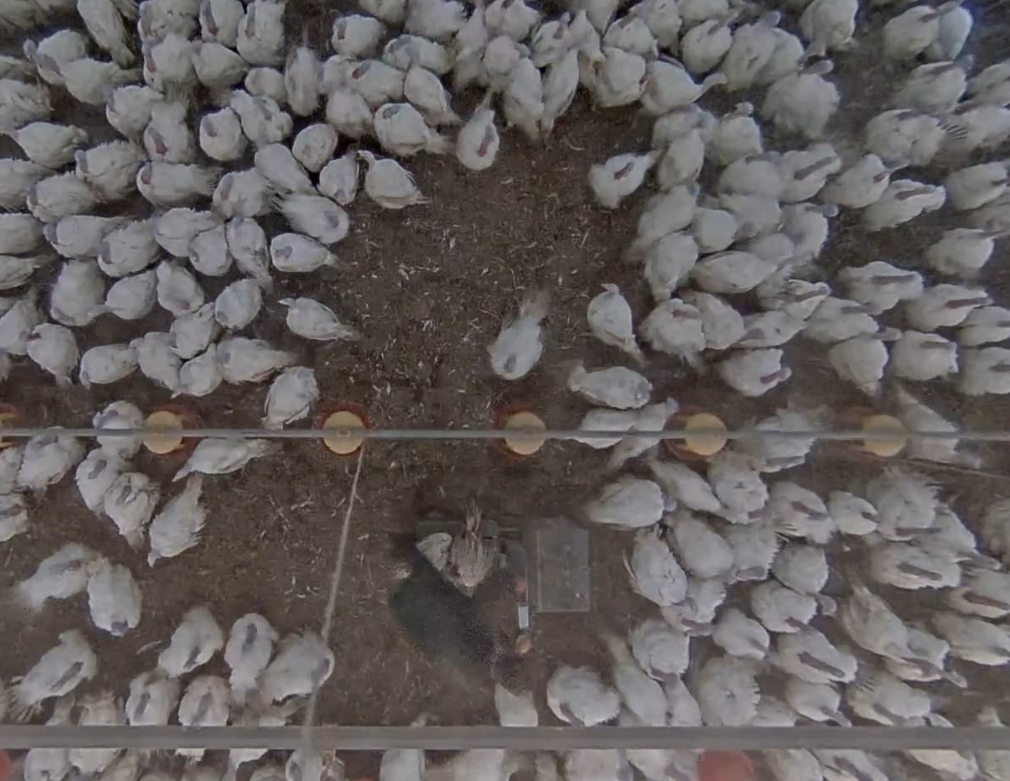
\includegraphics[width=\textwidth, height=5cm]{img/Verhaltensweisen/Kontrollgang Tierhalter Traube 2.png}
         \caption{Kontrollgang des Tierhalters.}
     \end{subfigure}
     \hfill
     \begin{subfigure}[b]{0.59\textwidth}
         \centering
         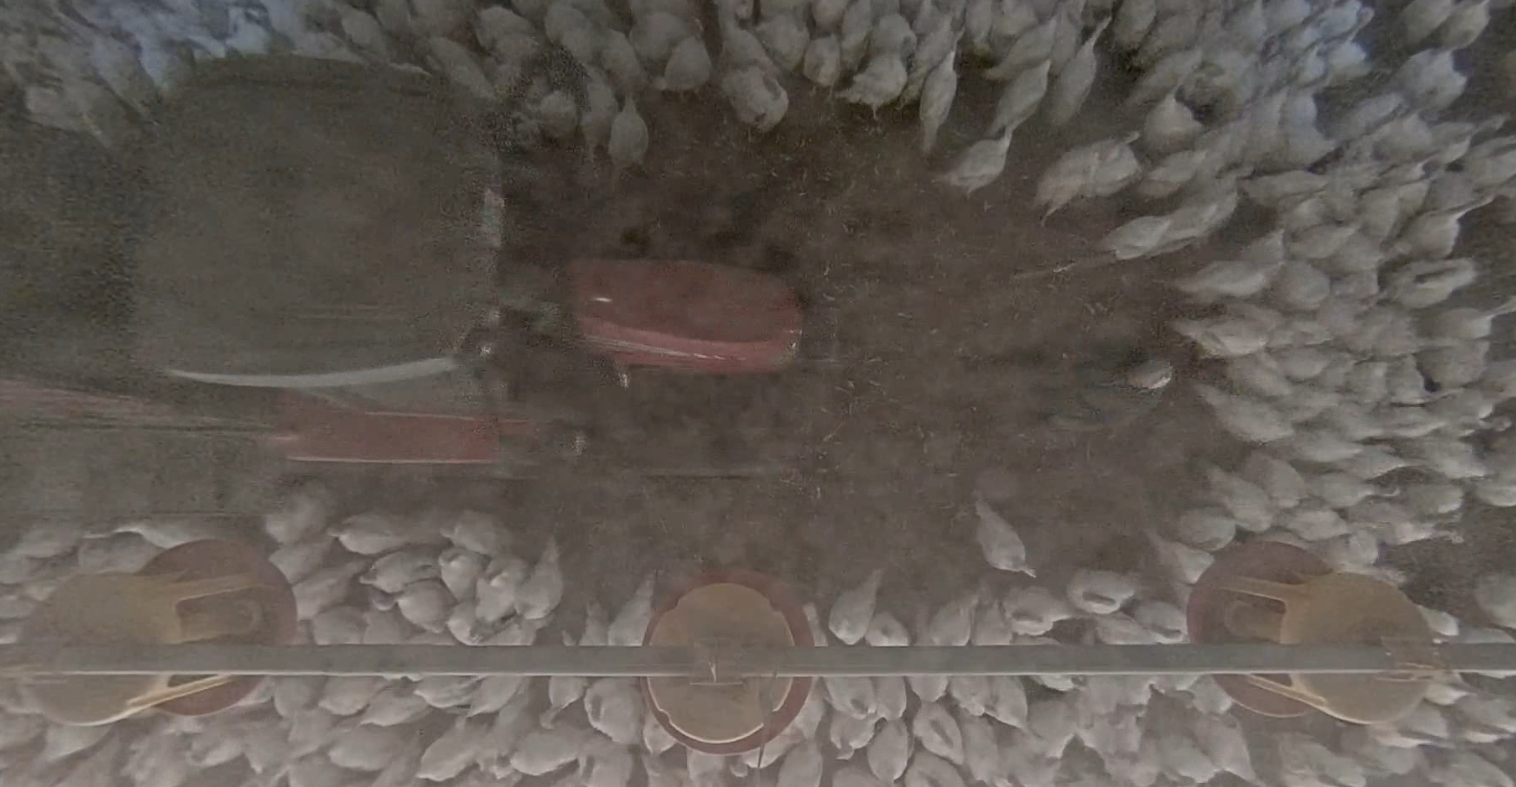
\includegraphics[width=\textwidth, height=5cm]{img/Verhaltensweisen/Kontrollgang Tracktor Traube.png}
         \caption{Einstreuung von Stroh mit Traktor.}
     \end{subfigure}
     \caption[Ausschnitte aus Kontrollgangereignissen.]{Ausschnitte aus Kontrollgangereignissen.}
     \label{fig:bspKontrollg}
\end{figure}


\par

\begin{quote}
\textbf{Kämpfe}\par
Ein Kampf entsteht ohne direkt ersichtlichen Auslöser. Ein Kampf beginnt meistens, indem sich zwei Tiere gegenüberstehen und sich gelegentlich versuchen anzupicken. Dies steigert sich meistens zu stärkeren Pickattacken. Dabei entwickeln die Tiere eine hohe Dynamik und bewegen sich umeinander. Oft passiert es, dass eine Pute die andere packt und um sich schleudert. Dadurch entstehen zirkulierende Bewegungsmuster. Die umliegenden Puten weichen den kämpfenden Tieren aus, wodurch eine \gfuss{Traube} entsteht. Auch Verfolgungen sind zu beobachten. Möchte eins der Tiere entkommen, jagt das andere diesem hinterher. Schafft es der Verfolger, die flüchtende Pute zu packen, wird der Kampf fortgesetzt. Die Verfolgungen finden mit hoher Dynamik statt. Es entstehen freie Flächen im Kanal der Fluchtbewegung. Ein Kampf muss nicht nur zwischen zwei Tieren stattfinden. Auch mehrerer Tiere können an einem Kampf beteiligt sein. Ebenfalls können die kämpfenden Tiere wechseln. Schafft es ein Tier zu flüchten und der Verfolger findet dieses nicht mehr, kann es sein, dass der Verfolger auf das nächstbeste Tier losgeht. Auch kann ein bisher unbeteiligtes Tier sich dazu entscheidet, in den Kampf mit einzusteigen. Der Kampf endet plötzlich und so, wie er begonnen hat, ohne ersichtlichen Auslöser. Die Abbildung \ref{fig:bspKämpf} zeigt einige Ausschnitte aus Kämpfen.
\end{quote}

\begin{figure}[htb]
     \centering
     \begin{subfigure}[b]{0.55\textwidth}
         \centering
         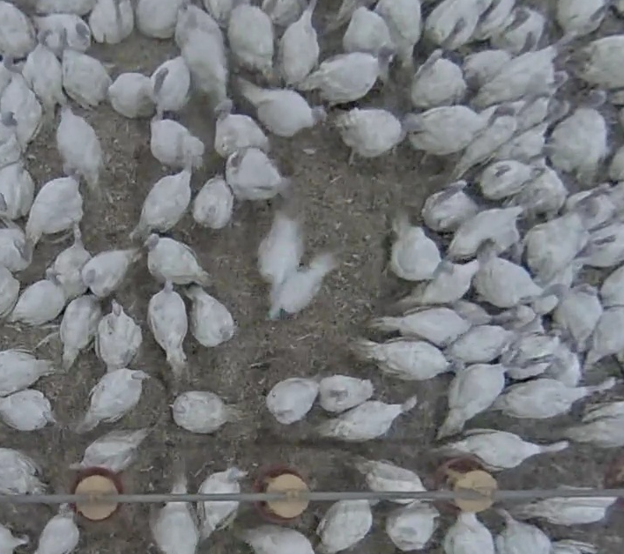
\includegraphics[width=\textwidth, height=6cm]{img/Verhaltensweisen/Kampf Traube.png}
         \caption{Kampf zwischen zwei Puten.}
     \end{subfigure}
     \hfill
     \begin{subfigure}[b]{0.44\textwidth}
         \centering
         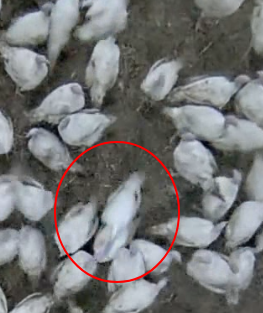
\includegraphics[width=\textwidth, height=6cm]{img/Verhaltensweisen/Kampf Verfolgung.png}
         \caption{Verfolgung eines flüchtenden Tieres.}
     \end{subfigure}
     \caption[Ausschnitte aus Kampfereignissen.]{Ausschnitte aus Kontrollgangereignissen.}
     \label{fig:bspKämpf}
\end{figure}

\par

Bei einem Kontrollgang treten dynamische Gruppenbewegungen auf, während Kämpfe durch dynamische Bewegungen vereinzelter Tiere geprägt sind. Bezogen auf den Kameraausschnitt ist bei einem Kontrollgang Dynamik in den meisten Bildbereichen zu beobachten. Kämpfe fallen durch lokale Dynamik in vereinzelten Bildbereichen auf. \par

Für diese Arbeit wurde jegliches Verhalten, was kein \textit{Kontrollgang} oder \textit{Kampf} ist, als \textit{Normalverhalten} deklariert. Der Begriff ist etwas irreführend gewählt, da \gfuss{Normalität} nicht näher definiert wurde. Jedoch sind Kämpfe und Kontrollgänge die auffälligsten Verhaltensweisen. Ebenfalls sind sie unerwünscht (\autoref{sec:Hintergrund}), weshalb der Fokus darauf gelegt wird, diese Verhaltensweisen vom restlichen Verhalten abzugrenzen. Das restliche Verhalten wird als \gfuss{Normal} bezeichnet. Die Definition der Merkmale von \textit{Normalverhalten} lässt sich aus diesem Grund als Abgrenzung von den anderen beiden Verhaltensweisen Formulieren.\dubpar

\begin{quote}
\textbf{Normalverhalten}\par
Während sich ein Kontrollgang durch eine globale hohe Dynamik auszeichnet und ein Kampf durch lokale hohe Dynamiken, so sind die Puten die meiste Zeit deutlich weniger aktiv. Bezogen auf die Bildbereiche der Kameras ruht sich ein Großteil der Tiere aus. Die Tiere sitzen stationär auf einer Position. Vermehrt tritt Aktivität rund um die Futterbahnen auf. Diese ist jedoch meistens nicht so dynamisch, wie in den anderen Verhaltensweisen.
\end{quote}
\par

Das Auftreten einer Verhaltensweise stellt für das geplante \gls{Modul} ein \gls{Ereignis} dar. Wie die Beschreibungen der Verhaltensweisen zeigen, basieren die charakterisierenden Merkmale vor allem auf der Bewegung der Tiere. Bewegung ist zeitabhängig. Die Merkmale der Verhaltensweise sind somit in einem Zeitraum zu beobachten. Ein \gls{Ereignis} wird also definiert durch einen Startzeitpunkt und einen Endzeitpunkt. Innerhalb dieser zeitlichen Grenzen sind die Merkmale der jeweiligen Verhaltensweise zu beobachten. \par

Aus den Anforderungen (\autoref{sec:Meth Anforderungen}) ist bekannt, dass ein \gls{Klassifikation}[sproblem] zu lösen ist. Durch die Erkenntnis, dass sich die \gls{Ereignis}[se] innerhalb eines Zeitraums abspielen und dem Fakt, dass auch die Rohdaten in Zeitreihen strukturiert sind (\autoref{sec:Meth RohDat}) wird deutlich, dass es sich bei der Aufgabe um eine \gls{Klassifikation} von Zeitreihen handelt.\par

\subsection{Aufbau des Gesamtkonzepts}
Die Aufgabe wurde definiert, die Rohdaten sind bekannt, das Format und die Merkmale der Verhaltensweisen wurden untersucht und die Modulanforderungen wurden formuliert. Mit diesem Wissen ist ein Gesamtkonzept für das \gls{Modul} zu entwicklen. Die Abbildung \ref{fig:GesKonzpt} zeigt dieses Konzept.

\begin{figure}[htb]
    \centering
    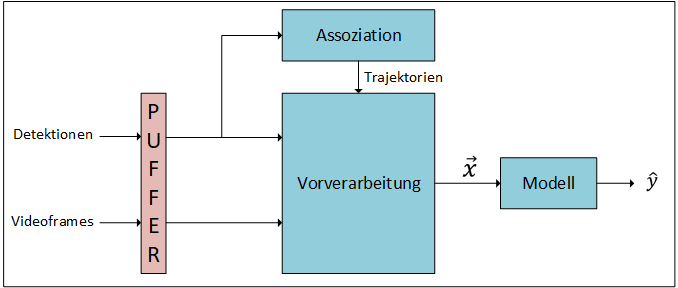
\includegraphics[width=0.9\textwidth]{img/Grafiken/Gesamtkonzept start.png}
    \caption{Gesamtkonzept des \gls{Modul}[s].}
    \label{fig:GesKonzpt}
\end{figure}


Ein Strom von Rohdaten fließt in das \gls{Modul}. Die \gls{Detektion}[sdaten] werden dem \gls{Assoziation}\glsdisp{Modul}{smodul} übergeben. Dieses generiert Trajektorien. Die Rohdaten und die Trajektorien fließen in einer Vorverarbeitung zusammen. Hier werden die \gls{Feature}[s] aus den Rohdaten extrahiert und konstruiert (\autoref{sec:ML FeatExtr}), die in der \gls{Feature}-Selektion (\autoref{sec:ML FeatSelect}) ausgewählt wurden. Nach der Vorverarbeitung wird der \gls{Featurevektor} dem ausgewählten (\autoref{sec:ML ModellSelect}), konfigurierten (\autoref{sec:ML HyperPara}) und trainierten (\autoref{sec:ML Metriken, Valid}) Modell übergeben. Das Modell schätzt, welche Verhaltensweise in der Probe zu beobachten ist und gibt ein \gls{Label} aus, das die Klassenzugehörigkeit eindeutig bestimmt. Dieses \gls{Label} ist auch die Ausgabe des \gls{Modul}[s]. \par

Da Zeitreihen \glsdisp{Klassifikation}{klassifiziert} werden müssen, ist die Vorverarbeitung der Rohdaten modellabhängig (\autoref{sec:sequenzen ML}). Nicht alle Modelle können Sequenzen direkt Verarbeiten. Wie \autoref{sec:Meth Nutzwert} zeigt, besitzen die vielversprechendsten Modelle kein Sequenzverständnis. Das Modell muss \gls{Feature}[s] erhalten, welche die Information der Zeitreihe komprimieren. Der Pufferspeicher ist dazu da, die einzelnen Zeitschritte der sequenziellen Rohdaten zu speichern. Sobald genügend Zeitschritte vorhanden sind, werden die Rohdaten an die Vorverarbeitung weitergegeben. Dort wird die gepufferte Sequenz zu einem einzelnen Datenpunkt komprimiert. 
\section{Bewertung des MOT-Systems}
Mit eine \gls{MOT} System sollen \gls{Trajektorie}[n] generiert werden um diese für \gls{Feature}[s] zu nutzen. In \ref{sec:Meth DefAufgabe} wird dargestellt, dass die Merkmale der Verhaltensweisen stark auf der Bewegung der Puten basieren. Über die \gls{Trajektorie}[n] sollen diese Informationen extrahiert werden können. Um das zu gewährleisten muss das \gls{MOT} System gut genug sein, um die Bewegungsmerkmale jeglicher Verhaltensweisen zu erfassen. Dies ist durch die Bewertung des \gls{MOT} Systems zu überprüfen. \par

Für die Evaluation des \gls{MOT} Systems ist eine \gls{Ground Truth} notwendig. Da die Evaluation Gültigkeit für einen sehr konkreten Anwendungsfall haben soll, ist es sinnvoll eine anwendungsbezogene \gls{Ground Truth} zu verwenden, anstatt Benchmarking Datensätze. \gls{Ground Truth}[s] für zwei Ereignisse wurden bereits vor dieser Arbeit erstellt. Wie in \ref{sec:MOT GT} dargestellt ist die Erstellung einer qualitativ hochwertigen \gls{Ground Truth} herausfordernd. Um die Aussagekraft der Evaluation beurteilen zu können, wird die Qualität der \gls{Ground Truth} diskutiert. \par

Für das \glsdisp{Assoziation}{Assoziationsmodul} ist ein Algorithmus auszuwählen. Zur Auswahl steht der \acrshort{SORT} Algorithmus (\ref{sec:MOT SORT}) und eine modifizierte Variante des Crocker-Grier Linking Algorithmus (\ref{sec:MOT CrockGrier}). Die Modifikationen werden in \ref{sec:Meth CrockGrieMods} erläutert. Für das Gesamtsystem ist zu Bewerten, welcher der Algorithmen die besten \gls{Feature}[s] gewährleisten kann. \par

Während der Versuche werden die Laufzeiten der Algorithmen gemessen, da diese relevant sind im Bezug auf die Echtzeitfähigkeit des Moduls. 


\subsection{Diskussion der Ground Truth Qualität} \label{sec:Meth GT Quali}
Noch vor dieser Arbeit sind zu zwei Ereignissen \gls{Ground Truth}[s] erstellt worden. Ein Kampfereignis und ein Kontrollgangereignis. Die Ereignisse sind jeweils eine Minute lang. Das Kampfereignis umfasst 91 \gls{Frame}[s], das Kontrollgangereignis umfasst 98 \gls{Frame}[s]. Dadurch ergiebt sich eine durchschnittliche \gls{Frame}[rate] von 1,6 \gls{Frame}[s] pro Sekunde. Die Ereignisse wurden von unterschiedlichen Personen bearbeitet.  \par

Die Herausforderungen, die die Erstellung einer qualitativ hochwertigen \gls{Ground Truth} mit sich bringt, waren zum Zeitpunkt der Erstellung nicht bewusst. Aus diesem Grund wurden keine klar definierten Regeln festgelegt, wie mit Mehrdeutigkeiten und anderen komplizieren Situationen umzugehen ist. Ganz ohne Regeln erfolgte die Erstellung jedoch nicht. Im Vorfeld wurde definiert, dass jedes Tier mit einer rechteckigen \gls{Bounding Box} zu \glsdisp{Detektion}{detektieren} ist. Die \gls{Bounding Box} soll das Tier möglichst eng, aber vollständig umschließen. Tiere sollen möglichst auch nach Verdeckungen korrekt \glsdisp{Assoziation}{assoziiert} werden. \par 

Bei der Überprüfung der \gls{Ground Truth} viel auf, die \gls{Detektion} funktionierte relativ zuversichtlich. Auch die \gls{Lokalisation} ist zufriedenstellend, auch wenn Schwankungen zu erwarten sind. Schwächen sind vor allem bei Mehrdeutigkeiten vorhanden. Die \gls{Detektion} bei teilweisen Verdeckungen ist inkonstant. Auch haben die unterschiedlichen Bearbeiter mehrdeutige Situationen unterschiedlich gelöst. Dadurch ist zu erwarten, dass Unsicherheiten in der Bewertung des \gls{Detektion}[smoduls] entstehen. Die Überprüfung zeigte, dass die \gls{Ground Truth} tendenziell eher Übermäßig optimistische Erwartungen an die \gls{Detektion} stellt. Bei teilweisen Verdeckungen wurde ein Tier länger \glsdisp{Detektion}{detektiert}, als es das \gls{Detektion}[smodul] tat. Somit ist mit einer vermehrten Anzahl von falsch negativen \gls{Detektion}[en] (\ref{sec:MOT Fehlertypen}) zu rechnen. \par

Die niedrige \gls{Frame}[rate], sowie die hohe Tierdichte im Stall, sorgten dafür das sich Tiere teilweise nur schwer auseinander halten ließen. Dadurch ist mit Unsicherheiten in der Evaluation des \gls{Assoziation}[smoduls] zu rechnen. 

Es ist empfehlenswert, dass das \gls{Detektion}[smodul] mit Daten trainiert wird, die aus der gleichen Quelle stammen wie die \gls{Ground Truth}. Das stellt eine faire Bewertung sicher, da keine diskrepanz vorhanden ist zwischen dem was das \gls{Detektion}[smodul] lernt und dem was die Evaluation von ihm fordert. Dies war hier nicht möglich, da die \gls{Detektion} bereits abgeschlossen war als die \gls{Ground Truth} erstellt wurde. Dadurch ist mit Unsicherheiten der Bewertung des \gls{Detektion}[smoduls] und des \gls{Lokalisation}[smoduls] zu rechnen.\par

Mit Fehlern in einer \gls{Ground Truth} ist zu rechnen. Um dennoch stabile Ergebnisse zu erhalten wird empfohlen mehrere \gls{Ground Truth}[s] zu verwenden und die Ergebnisse zu mitteln. Für die Bewertung bezogen auf den Anwendungsfall stehen jedoch nur zwei \gls{Ground Truth} Datensätze zur Verfügung. Das kann die Stabilität der Wertungen negativ beeinflussen.


\subsection{Modifikation des Crocker-Grier Linking Algorithmus} \label{sec:Meth CrockGrieMods}
Der grundlegende Aufbau des Crocker-Grier Linking Algorithmus ist in \ref{sec:MOT CrockGrier} erläutert. Die Modifikationen erfolgten bereits vor dieser Arbeit. Sie werden hier erläutert, um die Nachvollziehbarkeit der Arbeitsweise zu ermöglichen. \par

Bei der Anwendung der ursprünglichen Form des Crocker-Grier Linking Algorithmus auf Ereignisse im Putenmaststall, kam es zu Problemen. Die maximale Distanz \(l\) die ein Objekt zwischen zwei \gls{Frame}[s] zurücklegen darf, um korrekt \glsdisp{Assoziation}{assoziiert} werden zu können, wird von den Tieren oftmals nicht eingehalten. Gerade bei dynamischen Ereignissen legen die Puten in kürzerer Zeit, weitere Strecken zurück. Dies ist auch der niedrigen \gls{Frame}[rate] und hohen Tierdichte geschuldet. Durch die Verletzung von \(l\) entstehen \gls{Assoziation}[sfehler] (\ref{sec:MOT Fehlertypen}). Durch die Vergrößerung von \(l\) entstehen größere Netzwerke. In der Anwendung wurden die Netzwerke schnell so groß, dass die Rechenzeit unpraktikabel wurde.\par

Um diesen Problemen zu begegnen wurde eine iterative \gls{Assoziation} umgesetzt. Diese durchläuft mehrere Stufen, in denen die \gls{Assoziation} wiederholt wird. Bei jeder Iteration wird \(l\) vergrößert. Korrekte \gls{Assoziation}[en] werden in den folgenden Stufen nicht mehr betrachtet. Insgesamt werden drei Iterationen durchlaufen. Die Abbildung \ref{fig:funkCrockGrierMod} zeigt die Auswirkungen dieses Ansatzes. In der ersten Stufe werden vor allen stationäre Puten \glsdisp{Assoziation}{assoziiert}. Diese werden in den folgenden Stufen nicht mehr betrachtet. Dadurch wird der Abstand zwischen den zu \glsdisp{Assoziation}{assoziierenden} Objekten größer und korrekte \gls{Assoziation}[en] sind auch mit einem größeren \(l\) zu erwarten. Auch die Größen der entstehenden Netzwerke sind besser handhabbar. 

\emptyFigure{Stufen des Trackings, aus BA nehmen}{fig:funkCrockGrierMod}
\todo{Abbildung fehlt}

Gerade bei hoch dynamischen Ereignissen passiert es, dass in frühen Stufen nur wenige \gls{Assoziation}[en] getätigt werden können. Dadurch entstehen wieder mehr \gls{Assoziation}[sfehler]. Auch ist nicht mehr zu gewährleisten, dass der Rechenaufwand handhabbar bleibt. Aus diesem Grund wird in diesen Situationen das adaptive Verfahren angewendet, was in der \gls{Bibliothek} \textit{Trackpy} \cite{Allan.2023} implementiert ist. Dadurch wird sichergestellt, dass die Netzwerke eine Maximalgröße nicht überschreiten und der Rechenaufwand bleibt handhabbar. \par

Ziel ist es konstante \gls{Trajektorie}[n] zu generieren. Durch die Iterationen der Stufen können jedoch \gls{Fragmentation}[sfehler] provoziert werden. Das ist in der Abbildung \ref{fig:bspCrockGrierFrag} dargestellt. Unterbricht ein aktives Tier seine dynamische Bewegung für Wenige \gls{Frame}[s] und verweilt auf einer Position, dann werden die \gls{Assoziation}[en] dieser wenigen \gls{Frame}[s] bereits in einer früheren Stufe getätigt. Die \gls{Detektion}[en] der dynamischen Bewegung werden erst in höheren Stufen \glsdisp{Assoziation}{assoziiert}. Eine konstante \gls{Trajektorie} ist dann nicht mehr möglich, da das Verweilen des Tieres bereits aus der weiteren Betrachtung herausgenommen wurde. 

\emptyFigure{Fragmentation durch Stufen}{fig:bspCrockGrierFrag}
\todo{Abbildung fehlt}

Um solche Fehler zu vermeiden wurde ein Verifikatoinsmechanismus eingeführt, welcher evaluiert, ob eine \gls{Trajektorie} in einer bestimmten Stufe plausibel ist, oder nicht. ist die \gls{Trajektorie} plausibel, gilt sie als verifiziert und sie wird in das Ergebnis des \gls{MOT} Systems aufgenommen. Kann die \gls{Trajektorie} nicht verifiziert werden, dann kommen ihrer \gls{Detektion}[en] in die nächste Stufe. \gls{Detektion}[en], welche sich am Ende nicht in einer verifizierten \gls{Trajektorie} befinden, werden verworfen. Die Abbildung \ref{fig:TreeCrockGrierVerif} zeigt den Verifkationsmechanismus in Form eines Baumdiagramms. 

\emptyFigure{Verifikationsmechanismus}{fig:TreeCrockGrierVerif}
\todo{Abbildung fehlt}

Für die Verifikation wird das Video des Ereignisses mit herangezogen. Bei diesem wird ermittelt wie sich die Pixeln von \gls{Frame} zu \gls{Frame} verändern. Wenn \(\nommat{PIX}_t\) die Matrix aller Pixel in einem \gls{Frame} \(t\) ist, dann berechnet sich die Veränderung wie in \ref{eq:Pixelveränderung} dargestellt.

\begin{equation}
\text{Pixelveränderung} = \frac{abs(\nommat{PIX}_t - \nommat{PIX}_{t-1})}{\text{Pixelanzahl}}
\label{eq:Pixelveränderung}
\end{equation}

Dabei werden die Farbkanäle berücksichtigt. Ein \(Pixel \in \nommat{PIX}\) besitzt jeweils einen Kanal für rot, blau und grün. Diese können die Werte \(\{0,1,2, \dots, 255\}\) annehmen. Mathematisch lässt sich jeder Pixel als Vektor \(\nomvec{pix}\) betrachten. Der Wertebereich der Pixelveränderung somit \([0, 765]\), da \(3 \cdot 255 = 765\). \par

Der Verlauf der Pixelveränderung wird für das Ereignis ermittelt. Sie dient als Aktivitätsindikator. Eine \gls{Trajektorie} muss nicht über das gesamte Ereignis verlaufen. Es wird der Zeitraum betrachtet, in dem die \gls{Trajektorie} aktiv war. Für diesen Zeitraum wird die mittlere Pixelveränderung berechnet und die Standdardabweichung. Diese Werte dienen dazu um zu beurteilen, ob das Geschehen im Stall insgesamt Dynamisch ist, oder nicht. Bei einem dynamischen Geschehen, wie bei einem Kontrollgang, ist es sinnvoll die \gls{Detektion}[en] bei einem größeren \(l\) zu betrachten, da \gls{Fragmentation}[sfehler] wahrscheinlicher sind. \par

Die mittlere Geschwindigkeit aller \gls{Trajektorie}[n] wird berechnet und die Geschwindigkeit der individuellen \gls{Trajektorie}[n] wird damit verglichen. Liegt die Geschwindigkeit auffällig höher, als die mittlere Geschwindigkeit, wird das Potential für \gls{Fragmentation}[sfehler] als höher eingestuft und die \gls{Detektion}[en] werden in der nächsten Stufe erneut beurteilt. \par

Das letzte Verifikationskriterium ist die Schrittanzahl der \gls{Trajektorie}[n]. Von \gls{Trajektorie}[n], die über viele \gls{Frame}[s] verlaufen ist tendenziell zu erwarten, dass sie konstanter sind. Somit fordert der Verifikationsmechanismus eine minimale \gls{Frame}[anzahl], oder Anzahl von Zeitschritten.\par

Die Die Verifikationskriterien der unterschiedlichen Stufen sind dynamisch. Da in höheren Stufen eine höhere Fehleranfälligkeit erwartet wird, sinkt die minimale \gls{Frame}[anzahl], um nicht zu viele \gls{Trajektorie}[n] auszusortieren. Auch die Toleranzschranken für die Dynamik steigen, da in den höheren Stufen mehr Dynamik erwartet wird. \par



\subsection{Methodisches Vorgehen der MOT Evaluationen}
Für die Evaluation stehen zwei \gls{Ground Truth} Ereignisse zur Verfügung. Ein Kampfereignis und ein Kontrollgangereignis (\ref{sec:Meth GT Quali}). Die Algorithmen, zwischen denen Auszuwählen ist sind der \acrshort{SORT} Algorithmus (\ref{sec:MOT SORT}) und die modifizierte Variante des Crocker-Grier Linking Algorithmus (\ref{sec:Meth CrockGrieMods}). Die Evaluation wird mittels der \gls{HOTA} Metrik (\ref{sec:MOT HOTA}) durchgeführt, da mit dieser Metrik die fairste Bewertung zu erwarten ist und die genausten Fehleranalysen. Die \textit{\gls{IDF1}-Metrik} und die \textit{\acrshort{CLEAR} \gls{MOT}} Metriken werden jedoch angegeben, da sie etablierter sind als \gls{HOTA}. Für die Berechnung der Metriken wird die Software \textit{TrackEval} benutzt \cite{TrackEval.2020}. Diese ist die offizielle Evaluationsoftware der \textit{MOTChallenge} und steht als Open-Source Code zur Verfügung. Mit der Nutzung von \textit{TrackEval} wird sichergestellt, dass die Metriken korrekt berechnet werden. \par

Als erstes wird für beide Algorithmen die Gesamtperformance bewertet. Dazu werden die beiden Algorithmen auf die Ereignisse angewendet zu denen \gls{Ground Truth}[s] vorhanden sind. Für jeden \gls{Assoziation}[salgorithmus] ist anschließend ein Trackingergebnis vorhanden. Dieses beinhaltet die \gls{Trajektorie}[n]. Gespeichert werden die Trackingergebnisse als txt-Datei. Die Formatierung erfolgt angepasst an \textit{TrackEval}, gemäß \cite{MOT15}. Anschließend werden die Metriken berechnet. Wie \textit{TrackEval} auf eigene \gls{MOT} Systeme und mit eigenen \gls{Ground Truth}[s] anzuwenden ist, ist in der Dokumentation erläutert \cite{TrackEval.2020}. Die Evaluation der beiden Ereignisse wird gemittelt. Die Ergebnisse der beiden Algorithmen lassen sich vergleichen. Neben den Wertungen der \gls{HOTA} Metrik, erstellt \textit{TrackEval} einen Plot. Dieser zeigt den Verlauf der Wertungen über \(\alpha\). Die Abbildung \ref{fig:MPNTrack} zeigt einen solchen Plot. Dieser ist einem \gls{MOT} System namens \textit{MPNTrack} entnommen, welcher bei der \textit{MOTChallenge} 2016 und 2017 angetreten ist. Dieser ist hier zu Beispielzwecken angeführt. 

\emptyFigure{MPNTrack MOT17 bsp}{fig:MPNTrack}
\todo{Abbildung fehlt}

Während der Generation der Trajektorien werden die Laufzeiten der Algorithmen gemessen. Ebenfalls werden weitere Laufzeitmessungen durchgeführt, bei denen die Länge der Ereignisse stärker zu variieren sind. Dadurch ist ein Vergleich der Laufzeiten möglich und auch wie die Laufzeiten im Bezug auf die Ereignisslänge Skalieren.\par 

Als nächstes ist zu überprüfen, ob die \gls{Assoziation}[salgorithmen] alle Verhaltensweisen 
gleich gut \glsdisp{Assoziation}{assoziiert} bekommen. Dazu wird jedes Ereignis unabhängig von einander evaluiert.\par

\section{Nutzwertanalyse zur Vorauswahl von Machine Learning Modellen} \label{sec:Meth Nutzwert}
Für das \gls{Modul} zur Verhaltensklassifizierung wird ein Algorithmus des \glsdisp{ML}{maschinellen Lernens} benötigt. Die Auswahl eines passenden Algorithmus ist oftmals nur durch ausprobieren verschiedener Algorithmen möglich. Um Zeit einzusparen ist es Sinnvoll die Auswahl einzugrenzen \ref{sec:ML ModellSelect}. Diese Eingrenzung wird hier mittels einer Nutzwertanalyse durchgeführt. \par

Eine Nutzwertanalyse ist eine Methode zur Entscheidungsfindung, bei welcher Entscheidungsalternativen mittels einer Wertung verglichen werden \cite{Kuhnapfel.2021}. Sie ist jedoch anfällig für eine subjektive Bewertung der Entscheidungsalternativen. Aus diesem Grund wird sie hier nur für eine Eingrenzung der Auswahl verwendet und nicht für eine finale Entscheidung. Bei einer Nutzwertanalyse werden Kriterien ausgewählt, anhand derer die Alternativen bewertet werden. Diese Kriterien erhalten eine Gewichtung, welche ihre Wichtigkeit verdeutlicht. Die Gewichte werden in Prozent angegeben und ergeben kumuliert 100 \%. Für eine Alternative wird der Erfüllungsgrad in Bezug auf ein Kriterium angegeben. Für diesen Erfüllungsgrad ist eine Skala notwendig, bspw. \(\{1,2,\dots,10\}\). Diese Skala wird für alle Kriterien verwendet. Der Grad der Erfüllung wird für jede Alternative in Bezug auf alle Kriterien angegeben und Gewichtet. Die Summe der gewichteten Erfüllungswerte einer Alternative sind der Nutzwert dieser Alternative. Die Abbildung \ref{fig:bspNutzwertanalyse} zeigt beispielhaft eine Nutzwertanalyse.

\emptyFigure{Nutzwertanalyse BSP}{fig:bspNutzwertanalyse}
\todo{Abbildung fehlt}


\subsection{Auswahl der Kriterien}
Zunächst werden die Kriterien vorgestellt mit denen die Nutzwertanalyse durchgeführt werden soll. Diese sind Ausgewählt in Bezug auf die Aufgabe und die Rahmenbedingungen. Als Bewertungsskala werden die Werte \(\{1,2,\dots,10\}\) verwendet. Wie die Skala an die Kriterien angesetzt wird, wird erläutert. Ebenfalls erfolgt eine Einschätzung der Wichtigkeit.\par

\textbf{Rechenaufwand:}\\
Die Anforderungen an die Rechenleistung der Algorithmen können sehr unterschiedlich sein. Rechenleistung 
steht jedoch nur begrenzt zur Verfügung. Es stehen zwei baugleiche Rechner zur Verfügung. Die Prozessoren 
habe 16 Kerne und sie haben eine maximale Taktfrequenz von 5.10 GHz. Als Grafikkarte steht nur die der 
Hauptplatine zur Verfügung. Bezogen auf die Skala bedeuten höhere Werte eine geringere Anforderung an die Rechenleistung. Das Kriterium ist als wichtig einzustufen.\par

\textbf{Datenmenge:}\\
Gerade komplexe Modelle wie im \gls{Deep Learning} benötigen eine große Datenmenge. Wie in \ref{sec:Meth Datensatz} genauer beschrieben wird, ist die Datenmenge relativ klein. Dadurch entsteht gefahr für \gls{Overfitting}, gerade bei komplexen Modellen. Bezogen auf die Skala bedeuten höhere Werte eine geringere Anforderung an die Datenmenge. Die Datenmenge hat einen sehr großen Einfluss und das Kriterium ist als sehr wichtig einzustufen. \par

\textbf{Sequenzverständins:}\\
Bei der Aufgabe handelt es sich um ein \gls{Klassifikation}[sproblem] von Zeitreihen (\ref{sec:Meth DefAufgabe}). Gutes Sequenzverständnis wäre eine nützliche Fährigkeit des Modells (\ref{sec:sequenzen ML}). Höhere Werte auf der Skala bedeuten ein besseres Sequenzverständnis. Die Fähigkeit ist sehr relevant für die Aufgabe, jedoch bestehen Möglichkeiten Sequenzen auch mit einfacheren Modellen zu verarbeiten. Aus diesem Grund ist das Kriterium nicht Entscheidend und als mittelmäßig wichtig zu gewichten. \par

\textbf{Komplexität des Anwendens:}\\
Komplexere Modelle sind i.d.R. auch komplexer Anzuwenden. Da in Bezug auf diese Arbeit, wenig Vorerfahrung mit \glsdisp{ML}{machniellem Lernen} vorhanden ist und der Zeitrahmen begrenzt ist, ist eine einfache Anwendbarkeit des Modells Vorteilhaft. Eine niedrige Komplexität erzielt auf der Skala einen höheren Wert. Aus den Zeit und Erfahrungsgründen ist das Kriterium relevant, jedoch ist das Ziel ein möglichst gutes Modell zu erhalten. Deshalb sollte das Kriterium nicht Entscheidungsgebend sein. Es wird als geringfügig wichtig gewichtet. \par

\textbf{Modellierfähigkeit:}\\
Modelle des \gls{Deep Learning} haben eine sehr hohe Modellierfähigkeit, während eine lineare Regression nur wenig komplexe Zusammenhänge modellieren kann. Es ist jedoch einfacher ein komplexeres Modell durch Regularisierung in seiner Modellierfähigkeit zu beschneiden, als ein zu einfaches Modell zu verwenden. Deshalb wird eine hohe Modellierfähigkeit mit hohen Werten der Skala bewertet. Eine sehr hohe Modellierfähigkeit sehr hoch zu Bewerten, kann sich verzerrend auf die Nutzewertanalyse auswirken. Eine sehr hohe Modellierfähigkeit kann zu \gls{Overfitting} führen, wenn die Rahmenbedingungen nicht Stimmen, wir z.B. eine ausreichende. Datenmenge. Um solchen Verzerrungen entgegen zu wirken, wird das Kriterium als geringfügig wichtig eingestuft. \par

\textbf{Geschwindigkeit der Schätzung:}\\
Da das \gls{Modul} für die Verhaltensklassifikation Echtzeitfähigkeit besitzen soll, ist die Geschwindigkeit der Ergebnisfindung des Modells wichtig. Eine hohe Geschwindigkeit erzielt hohe Wertungen auf der Skala. Die Geschwindigkeit der Schätzung ist sehr relevant für das Gesamtkonzept. Jedoch ist der Anwendungsfall nicht kritisch, weshalb keine harten Toleranzgrenzen für die Echtzeitbedingung gelten. Die Wichtigkeit ist deshalb als geringfügig wichtig eingestuft. \par

In der Tabelle \ref{tab:NWAKriterien} ist eine Übersicht der Kriterien zu sehen. Die Wichtigkeit wurde versucht zu quantisieren. Ebenfalls ist Dargestellt wie die Skalen verlaufen.


\begin{table}[ht]
    \centering
    \begin{tabular}{|l|r|r|}
         \hline
         \textbf{Kriterium}                      & \textbf{Skala \(\{1,2,\dots,10\}\)}    & \textbf{Gewichtung}\\
         \hline
         Rechenaufwand                  & hoch \dots niedrig            & 25 \%\\
         \hline
         Datenmenge                     & hoch \dots niedrig            & 34 \%\\
         \hline
         Sequenzverständnis             & niedrig \dots hoch            & 17 \%\\
         \hline
         Komplexität des Anwendens      & hoch \dots niedrig            & 8 \%\\
         \hline
         Modellierfähigkeit             & niedrig \dots hoch            & 8 \%\\
         \hline
         Schätzungsgeschwindigkeit  & niedrig \dots hoch            & 8 \%\\
         \hline
         \textbf{Summe}                 &                               & 100 \%\\
         \hline
    \end{tabular}
    \caption{Übersicht über die Kriterien für die Nutzwertanalyse und ihre Gewichte.}
    \label{tab:NWAKriterien}
\end{table}

\subsection{Abwägung der Algorithmen}
Die Algorithmen zwischen denen abgewägt werden soll, sind in \ref{sec:ML Algorithmen} vorgestellt. Sie werden hier im Bezug auf die Kriterien diskutiert. Abschließend wird die Nutzwertanalyse präsentiert und die Auswahl der Algorithmen eingegrenzt. \par

\textbf{k-Means Algorithmus}\\
Der k-Means Algorithmus besitzt kein direktes Sequenzverständnis. Doch es bietet sich an Distanzmetriken für Zeitreihen einzusetzen, um eine Clusteranalyse anhand der Ähnlichkeit der zeitreihen durchzuführen. Auch die Option komprimierte \gls{Feature}[s] zu verwenden ist gegeben. Der Algorithmus ist an für sich nicht besonders Anspruchsvoll in seinem Rechenaufwand. In Kombination mit Distanzmetriken für Sequenzen, können diese dafür sorgen, dass der Aufwand steigt. Die Berechnung von solchen Distanzmetriken, wie Dynamik Time Warping kann Rechenaufwändig sein. Eine k-Means Clusteranalyse ist bereits mit einer relativ kleinen Datenmenge gut durchführbar. Die Anwendung ist prinzipiell sehr einfach, da meistens nur ein einziger \gls{Hyperparameter}, die Clusteranzahl benötigt wird. Jedoch liegt auch genau hier die Schwierigkeit. Die Clusteranzahl muss im Vorhinein bestimmt werden. Diese zu Ermitteln kann aufwendig sein. Implementationen des Algorithmus sind in verschiedenen Software-\gls{Bibliothek}[en] zu finden \cite{FabianPedregosa.2011}. Die Modellierfähigkeit ist begrenzt aus mehreren Gründen. Zum einen lernt das Modell unüberwacht, wodurch der Lernprozess nicht kontrollierbar ist. Das sorgt dafür, dass auch die Modellierung nur schwierig anzupassen ist. Zusätzlich ist das Vorgehen wenig komplex, wodurch wichtige Zusammenhänge in den \gls{Feature}[s] eventuell nicht gefunden werden. Von der Geschwindigkeit der Schätzung ist nicht davon auszugehen, dass sie problematisch seien wird.

\textbf{Hierarchisches Clustering}
Das hierarchische Clustering ist in den meisten Aspekten ähnlich einzustufen wie der k-Means Algorithmus. Der Hauptunterschied liegt darin, dass die Cluster selbst gefunden werden, ohne vorweg eingestellt werden zu müssen. Das macht die Anwendung einfacher als beim k-Means Algorithmus.\par

\textbf{Logistische Regression}
Die Logistische Regression ist, wie in \ref{sec:ML Algorithmen} dargestellt im Grunde ein lineares Modell. Das macht die Berechnung relativ einfach. Der Rechenaufwand ist dem entsprechend nicht sonderlich hoch. Jedoch ist das Modell dadurch auch nicht besonders komplex, was die Modellierfähigkeit begrenzt. Da es jedoch überwacht lernt und Regularisierung möglich ist, ist es deutlich Anpassbarer als k-Means und das hierarchische Clustering. Es ist in der Lage mit einer relativ kleinen Datenmenge auszukommen und Das Modell ist einfach anzuwenden. Auch die Dauer der Schätzung ist sehr gering zu erwarten, da die Berechnung des Ergebnisses im Kern mittels einer linearen Gleichung erfolgt. Reihenfolgen in Daten kann das Modell nicht berücksichtigen. Sequenzverständnis ist deshalb nur mit der Komprimierung der Zeitreihen möglich.\par

\textbf{Support Vector Machines}
\acrshort{SVM}[s] basieren im Kern auch auf einem linearen Modell, wodurch sie im Bezug auf den Rechenaufwand, die Datenmenge der Komplexität des Anwendens und der Schätzungsgeschwindigkeit ähnlich sind wie die logistische Regression. Da \acrshort{SVM}[s] jedoch durch Modifikationen auch in der Lage sind nicht-lineare Modelle zu erstellen ist die Modellierfähigkeit besser als bei der logistischen Regression. Dies kann jedoch den Rechenaufwand erhöhen.\par

\textbf{Random Forest}
Da das Random Forest Modell seine Entscheidungsbäume parallel erstellt, lässt es sich mit mehreren Prozessorkernen effizient erstellen. Da es jedoch mehrere einfache Modelle verwendet, ist der Rechenaufwand dennoch höher als bei der \acrshort{SVM} oder der linearen Regression. Dafür ist Modellierfähigkeit besser. Zu Konfigurtation des Modells sind mehr Hyperparameter einstellbar. Das macht die Anwednung etwas komplexer, als bei der SVM und der linearen Regression. In der Regel benötigt das Modell etwas mehr Daten als die linearen Modelle, jedoch ist die Modellkomplexität durch die Hyperparameter gut einstellbar, so dass eine geringe Datenmenge ausreichen kann. Die Schätzgeschwindigkeit ist höher zu erwarten als bei den linearen Modellen, da die Ergebnisfindung aus zwei Schritten besteht. Im ersten finden die einzelnen Bäume eine Lösung und im Zweiten wird die Mehrheit ermittelt. Das Sequenzverständnis ist genau so gut wie bei den linearen Modellen.\par

\textbf{Gradient Boosting}
Gradient Boosting ist Rechenintensiver als Random Forest. Durch die sequentielle Erstellung der Bäume ist das Training nicht parallelisierbar. In der Regel ist das Modell Modellierfähiger als Random Forest. Durch das erlernen wie es Fehler korrigieren muss, wird das Modell besser auf die Daten zugeschnitten, jedoch ist das Potenzial für Overfitting dadurch höher als bei Random Forest. In den anderen Kriterien ist eine ähnlich gute Performance zu erwarten wie bei Random Forest.\par

\textbf{Long Short Term Memory}
Der große Vorteil von LSTMs und Deep Learning für die Aufgabe ist, dass sie Sequenzen verstehen können. Dadurch muss nicht mit Informationsverlust durch Komprimierung gerechnet werden. Deep Learning Modelle sind extrem Modellierfähig, jedoch auch komplex anzuwenden, da sie viele Hyperparameter besitzen. Für einfachere Aufgaben sind jedoch auch Netzwerke möglich, die nur wenige Schichten haben, wodurch die Komplexität überschaubar bleibt. Dadurch das mehrere Schichten durchlaufen werden, ist mit einer erhöhten Dauer für die Ergebnisfindung zu rechnen. Deep Learning benötigt jede Menge Daten und viel Rechenleistung. 

\textbf{Gated Recurrent Unit}
Die GRU ist in den meisten Kriterien ähnlich zu bewerten wie das LSTM, aus den gleichen Gründen. Durch die reduzierte Komplexität der GRU ist mit einem etwas geringeren Rechenaufwand auszugehen. Auch die benötigte Datenmenge ist dadurch vermutlich etwas geringer.\ar

\begin{table}[ht]
\centering
\setlength{\tabcolsep}{11pt}
\caption{Nutzwertanalyse der Modelle}
\begin{tabular}{
    l
    S[table-format = 1.2]
    *{6}{S[table-format=2.0]} % Formatierung für die Zahlen ohne Dezimalstellen
    S[table-format=2.2]
    S[table-format=1.0]
  }
\toprule
Kriterien & 
\rotatebox{90}{Gewicht} & 
\rotatebox{90}{k-Means} & 
\rotatebox{90}{Hierarchisches Clustering} & 
\rotatebox{90}{Logistische Regression} & 
\rotatebox{90}{SVM} & 
\rotatebox{90}{Random Forest} & 
\rotatebox{90}{Gradient Boosting} & 
\rotatebox{90}{LSTM} & 
\rotatebox{90}{GRU}  \\
\midrule
Rechenaufwand               & 0,25 & 6 & 6 & 10 & 9  & 8 & 7 & 1  & 2 \\
Datenmenge                  & 0,34 & 9 & 9 & 9  & 9  & 8 & 8 & 1  & 2 \\
Sequenzverständnis          & 0,17 & 5 & 5 & 4  & 4  & 4 & 4 & 10 & 10 \\
Komplexität des Anwendens   & 0,08 & 5 & 7 & 7  & 7  & 6 & 6 & 2  & 2 \\
Modellierfähigkeit          & 0,08 & 1 & 1 & 5  & 6  & 7 & 8 & 10 & 10 \\
Schätzungsgeschwindigkeit   & 0,08 & 9 & 9 & 10 & 10 & 8 & 8 & 5  & 5 \\
\midrule
\addlinespace % Extra Abstand vor der letzten Zeile
Nutzwert & {--} & 6,6 & 6,8 & 8,0 & 7,8 & 7,1 & 6,9 & 3,7 & 4,2 \\
Rang & {--} & 6 & 5 & 1 & 2 & 3 & 4 & 8 & 7 \\
\bottomrule
\end{tabular}
\end{table}


\input{chapters/methodenentwicklung/Entwicklung eines Konzepts für die Verifizierung und das Labeling der Ereignisse}
\section{Zusammensetzung des Ursprungsdatensatzes}
\section{Konzept zur Feature-Extraktion}
\section{Anwendung der Methoden des Feature-Engineerings}
Über das Konzept in \autoref{sec:Meth FeatExtr} können Features aus den Rohdaten extrahiert werden. Im Vorfeld ist die Frage zu beantworten, welche Features extrahiert werden sollen. Diese Features werden in \autoref{sec:Meth ExtrFeaturesVors} vorgestellt. Mit den extrahierten Features als Grundlagen lassen sich weitere Features konstruieren (\autoref{sec:ML FeatExtr}). Welche Methoden zur Feature-Konstruktion verwendet werden, wird in \autoref{sec:Meth KonstrFeatures} erläutert.


\subsection{Vorstellung der extrahierten Features} \label{sec:Meth ExtrFeaturesVors}
Die charakteristischen Merkmale der Verhaltensweisen sind in \autoref{sec:Meth DefAufgabe} dargestellt. Diese waren teilweise bereits bekannt und teilweise sind sie erst während der Verifizierung aufgefallen. Dadurch ist Fachwissen vorhanden, um maßgeschneiderte Features zu entwerfen. Fachwissen ist ein großer Vorteil für den Entwurf von Features, wie in \autoref{sec:ML FeatExtr} erläutert. Es ist sinnvoll, Bias einzuführen in Bezug auf die charakteristischen Merkmale. Features können so konstruiert werden, dass sie darauf ausgelegt sind, bestimmte Aspekte der charakteristischen Merkmale zu erfassen. Ebenfalls ist durch das Fachwissen und das Wissen, dass die Zusammensetzung der Ereignisse Bias-behaftet ist (\autoref{sec:Meth Datensatz}), besser abzuwägen, ob bestimmte Features den vorhandenen Bias verstärken. Auch können Features entworfen werden, die gezielt versuchen, den Bias abzuschwächen. \par

Das soll an einem Beispiel verdeutlicht werden. Ein charakteristisches Merkmal von Kontrollgängen sind prägnante Gruppenbewegungen. Die Tiere drängen kollektiv in Richtung des Tierhalters. Somit kann der Drift der Bewegung aller Tiere ein interessantes Feature sein. Die Driftrichtung würde jedoch den Bias in den Daten verstärken, da diese vermutlich sehr abhängig vom Stallbereich ist. Da die Ereignisse jedoch nur aus zwei Stallbereichen stammen, ist dies ein Feature, das die Generalisierung hinsichtlich aller Stallbereiche beeinträchtigen würde. Ein besseres Feature wäre der Betrag der Driftgeschwindigkeit. Dieser ist ein Indikator für eine starke kollektive Bewegung in eine unbestimmte Richtung und damit unabhängiger vom Stallbereich. \par 

Für die Feature-Erstellung ist nochmal darauf hinzuweisen, dass die Merkmale einer Sequenz, also eines Ereignisses, zu einem einzelnen Datenpunkt komprimiert werden. Die Features benutzen immer einen einzigen Wert, um eine Information aus mehreren Zeitschritten zusammenzufassen. Ebenfalls sind möglichst numerische Features zu erstellen, da gerade einfachere Modelle mit diesen besser umgehen können als mit kategorischen Features. Im Anhang findet sich eine Tabelle mit ausführlichen Beschreibungen der Features, die mit dem Konzept aus \autoref{sec:Meth FeatExtr} für den Trainingsdatensatz extrahiert werden. Insgesamt sind dies 40 Features. Diese werden im weiteren Verlauf Basis-Features genannt, da die weiteren Features aus diesen konstruiert werden.\par


\subsection{Konstruktion der Features} \label{sec:Meth KonstrFeatures}
Da eine ausführliche Analyse und Auswahl der Features geplant sind, wird bei der Konstruktion der Fokus auf Masse gelegt. Features werden mittels aller Konstruktionsmethoden generiert, die in \autoref{sec:ML FeatExtr} vorgestellt sind. Bei der Durchführung ist festzustellen, dass einige der Basis-Features keine Information beinhalten. Die minimale Entfernung und Kurvigkeit sind in allen Ereignissen konstant null. Diese werden aus der Feature-Menge entfernt, somit reduziert sich die Anzahl der Basis-Features auf 38.\par

Zunächst werden Interaktionsfeatures erschaffen, indem die Features paarweise multipliziert werden, um ein neues Feature zu generieren. Auch die Multiplikation mit sich selbst ist darin eingeschlossen. Es entstehen 741 neue Features, wodurch die Featureanzahl auf 779 steigt. Mittels Gruppierung werden die 779 Features in Perzentile eingeteilt und als Perzentil-Features bezeichnet. Ebenfalls werden die Power-Transformationen auf die 779 Features angewendet. Die logarithmische Transformation wird mit der Basis 10 durchgeführt, da sie vor allem die Größenordnungen stauchen soll. Auch die Box-Cox-Transformation für alle 779 Features eingesetzt. \par

Bei der Berechnung der Perzentil-Features ist die normierte maximale Schrittanzahl nicht gruppierbar, auch nicht in der Interaktion mit sich selbst. Das liegt an Invarianz in der Verteilung, da der Wert meistens 1 beträgt. Deshalb fallen diese beiden Features heraus. Neun weitere Features lassen sich aufgrund geringer Varianz zwar nicht in Perzentile, dafür aber in Dezile einteilen. Da die Bezeichnung Perzentil-Features somit faktisch nicht mehr korrekt ist, werden sie als Quantil-Features bezeichnet. \par

Ziel der Gruppierungen und Power-Transformationen ist es, jegliche Features, die Informationen beinhalten können, unterschiedlich zu skalieren und zu formatieren. In der Feature-Auswahl soll untersucht werden, welche Methode die Informationen des jeweiligen Features am besten verpackt. Die Tabelle \ref{tab:FeatureMenge} zeigt die Feature-Mengen nach der Transformation.


\begin{table}[ht]
    \centering
    \caption{Übersicht über die Feature-Mengen pro Kategorie.}
    \begin{tabular}{|l|r|}
        \hline
        Feature-Kategorie & Anzahl\\
        \hline
        Basis & 38 \\
        Interaktion & 741\\
        Quantile & 777\\
        Logarithmisch & 779\\
        Box-Cox & 779\\
        \hline
        \hline
        Gesamt & 3114\\
        \hline
    \end{tabular}
    \label{tab:FeatureMenge}
\end{table}
\section{Methoden zur Feature-Auswahl, Hyperparametersuche und Modellauswahl} \label{sec:Meth FeatHypModSelect}
zwischen der Feature-Auswahl, dem Modellauswahl und der Hyperparamtersuche besteht ein enger Zusammenhang. Werden für die Feature-Auswahl modellabhängige Methoden verwendet, wie die Wrapper Methoden, muss ein Modell vorhanden sein, mit welchem sich die Methoden anwenden lassen. Um zwischen unterschiedlichen Modellen auszuwählen auf Basis ihrer Performance, ist eine Einstellung der Hyperparameter notwendig, damit die Modell auch fair bewertet werden. Ein Modell \(A\) wird beispielsweise mit einem Modell \(B\) verglichen. Die Hyperparameter sind noch nicht eingestellt. Modell \(A\) erzielt eine bessere Performance. Anschließend werden passende Hyperparameter gesucht. Anschließend zeigt ein weiterer Vergleich, dass nun Modell \(B\) die bessere Wahl ist. \par

Um also ein möglichst effektives Modell zu erhalten, ist eine Grobe Voreinstellung der Hyperparameter durchzuführen der Modelle durchzuführen. Anschließend wird eine Methode für die Feature-Auswahl angewendet. Da die Modelle vorhanden und eingestellt sind, darf diese modellabhängig, oder modellunabhängig sein. Anschließend kann die Performance der Modelle verglichen werden. Das beste wird ausgewählt und eine Feineinstellung der Hyperparameter wird durchgeführt. Das finale wird mit dem Testdatensatz überprüft und kann anschließend angewendet werden.\par

Da die Hyperparametersuche über die Optimierung des Validierungsergebnisses geschieht und dafür Modelle trainiert werden müssen, benötigt es hier bereits gute Features. Aus diesem Grund wird eine Vorauswahl der Features durchgeführt, um die Menge der Features einzugrenzen. Da uninformative Features Underfitting verursachen können und redundante Features Overfitting provozieren können, ist ein Vorauswahl sinnvoll, um eine aussagekräftige Einschätzung der Generalisierfähigkeit der Modelle zu erhalten. \par

Da die Datenmenge sehr begrenzt ist, wie in \ref{sec:Meth Datensatz} dargestellt, wird für die Validierung Cross-Validation angewendet (\ref{sec:ML Metriken, Valid}). Für das Training und das Testen wird der Datensatz aus \ref{tab:DataNachBalance} in ein Trainingsdatensatz und einen Testdatensatz aufgeteilt. 20 \% der Datenmenge wird für das Testen beiseite gelegt. Die Tabelle \ref{tab:TrainTestSplit} zeigt die Datenmangen die für Training und Testen zur Verfügung stehen.


\begin{table}[ht]
    \centering
    \caption{Aufteilung der Daten in Trainings- und Testdatensatz.}
    \begin{tabular}{|l|r|r|}
        \hline
        Datensatz & Datenmenge & Anteil \\
        \hline
        Trainingsdatensatz & 528 & 80 \%\\
        Testdatensatz & 132 & 20 \%\\
        \hline
        \hline
        Gesamt & 660 & 100 \%\\
        \hline
    \end{tabular}
    \label{tab:TrainTestSplit}
\end{table}

\subsection{Vorauswahl der Features} \label{sec:Meth FeatVorSele}
Zunächst werden die Filter-Methoden angewendet, da sie modellunabhängig Anwendbar sind. Dadurch entstehen  Feature Rangfolgen: eine für die Varianzanalyse und eine für die Gegenseitige Information. Jedoch ist die Qualität dieser Rangfolgen nicht überprüfbar ohne Modell. Aus diesem Grund wurde sich ein verfahren Überlegt, wie die Rangfolge der Filter-Methoden möglichst modellunabhängig evaluiert werden kann. \par

Es wird ein Modell genommen, bspw. die logistische Regression. Dieses bleibt unkonfiguriert. Es wird mit den Standardeinstellungen der \gls{Bibliothek} verwendet. Dieses bekommt inkrementell die Features, nach ihrer Rangfolge übergeben. In jeder Inkrementation wird das Modell trainiert und validiert. In der ersten Inkrementation wird das Modell also nur mit dem höchstrangigen Feature aufgebaut. In der zweiten Inkrementation mit den beiden höchstrangigen Features und in der Dritten mit den drei höchstrangigen Features. Validiert werden die Modelle mit der Metrik Accuracy und Cross-Validation. Somit entsteht ein Verlauf, der sich zweidimensional visualisieren lässt. Auf der y-Achse wird die Accuracy dargestellt und auf der y-Achse die Feature-Anzahl mit welcher das jeweilige Modell trainiert wurde. Die Abbildung \ref{fig:bspSättAccu} zeigt beispielhaft einen Linienplot der Accuracy. 

\emptyFigure{Beispiel eines Verlaufs der Accuracy im Bezug auf die Feature-Anzahl, für die Feature-Vorauswahl. Die Accuracy verläuft in eine Sättigung.}{fig:bspSättAccu}
\todo{Abbildung fehlt}

Die resultierende Betrachtung, lässt eine grafische Beurteilung der Feature-Auswahl zu. Auch multivariate Einflüsse werden hier betrachtet. Jedoch ist das vorgehen noch modellabhängig. Um die Ergebnisse zu verallgemeinern, wird der Verlauf der Accuracy für jedes Modell in der Vorauswahl gemessen. Die Werte werden anschließend gemittelt. Dadurch entsteht ein Verlauf der Accuracy, welcher sich nicht auf ein bestimmtes Modell bezieht. Die Methode ist also verwendbar, um eine Feature-Rangfolge möglichst modellunabhängig zu Beurteilen.\par

Wichtig zu Erwähnen ist, dass die Featurewerte für eineiige Modelle skaliert werden müssen, damit diese mit den Features Arbeiten können. Für die lineare Regression werden diese auf den Wertebereich [0;1] skaliert. Für die SVMs werden alle Features auf den Wertebereich [-1;1] skaliert.\par

Wie in der Abbildung \ref{fig:bspSättAccu} zu sehen ist, läuft die Genauigkeit in eine Sättigung. Ein solcher Verlauf zeigte sich allen durchgeführten Versuchen. Da die Messwerte schwanken, wird der Verlauf mit einer Sättingungslinie approximiert. Somit steht ein stabileres Maß für die Beurteilung und für Vergleiche zur Verfügung. Der Sättigungsverlauf deutet auf Redundanzen in den Features hin. Ab einer bestimmten Feature-Menge erhält das Modell keine neuen Informationen durch mehr Features. Das ist nicht verwunderlich, da alle Features auf den 38 Basis-Features aufbauen. Der Sättigungsverlauf ist praktisch für die Feature-Auswahl, da über den Punkt ab dem die Sättigung erreicht wird, eine optimale Feature-Menge bestimmt ist. \par

Da die Rangfolge der Filter-Methoden wie bereits erwähnt, durch eine univariate Beurteilung erfolgt, ist zu vermuten, dass sie nicht optimal ist. Eine Rangfolge, welche die Features multivariat beurteilt ist wünschenswert. Mit den Wrapper Methoden lassen sich Features auswählen, mit einem Verfahren was auch multivariate Zusammenhänge verücksichtigt. Die Wrapper Methoden erstellen jedoch keine Rangfolge. Es werden deshalb unterschiedliche Messreihen mithilfe der Wrapper Methoden aufgenommen. Die Ergebnisse der Messreihen sollen in eine Rangfolge der Features überführt werden.\par

Aus der Anwendung der Wrapper Methoden auf ein Modell und eine Feature-Menge ist eine binäre Wertung eines Features abzuleiten: \textit{Ausgewählt} oder \textit{nicht Ausgewählt}. Werden mehrere Wiederholungen durchgeführt in denen die Wrapper Methoden angewendet werden, bei denen die Zusammensetzung der Feature-Menge variiert wird und auch das Modell, so entstehen mehrere binäre Evaluationen eines Features. Aus diesen kann eine Gesamtwertung des Features abgeleitet werden. Die Tabelle \ref{tab:bspWrapScore} veranschaulicht dies an einem Beispiel und die Formel \ref{eq:Meth WrapperScore} zeigt die Berechnung der Wertung.

\begin{table}[h]
    \centering
    \caption{Beispiel einer Versuchsreihe zu dem Feature i, durch die Anwendung von Wrapper Methoden.}
    \begin{tabular}{|c|r|r|}
        \hline
        \multicolumn{3}{|r|}{\(Feature_i\)} \\
        \hline
        Versuch ID & Ausgewählt & Nicht Ausgewählt \\
        \hline
        0 & 1 & 0 \\
        1 & 1 & 0 \\
        2 & 0 & 1 \\
        3 & 1 & 0 \\
        4 & 0 & 1 \\
        5 & 1 & 0 \\
        \hline
        \hline
        Gesamt & 4 & 2 \\
        \hline
    \end{tabular}
    \label{tab:bspWrapScore}
\end{table}

\begin{equation}
W(x) = \frac{|\text{Ausgewählt}(x)|}{|\text{Ausgewählt}(x)| + |\text{Nicht Ausgewählt}(x)|} \rightarrow W(Feature_i)=\frac{4}{4+2} = 67\ \%
\label{eq:Meth WrapperScore}
\end{equation}

In der Formel \ref{eq:Meth WrapperScore} ist \(W(x)\) die Wertung eines Features \(x\). Zur Klarheit wird \(w\) im folgenden als \textit{Wrapper-Score} bezeichnet. Der Mechanismus der Wrapper-Score ist einfach. Wird ein Feature auch in unterschiedlichen Feature-Mengen und von unterschiedlichen Modellen oft ausgewählt, steigt der Wert. Das Maximum ist 1 und das Minimum 0. Features die in Kombination miteinander informativ sind, werden in der Hinsicht berücksichtigt, dass diese einen ähnlichen Wrapper-Score erzielen sollten. Sind sie sehr informativ, stehen sie gemeinsam weit oben in der Rangfolge. \par

Um eine aussagekräftige Rangfolge durch die Wrapper-Scores zu erhalten sind Messreihen aufzunehmen. Dazu sind mehrere Modelle zu benutzen. Verwendet werden eine klassische logistische Regression, eine lineare SVM und ein Random Forest Modell, ein Histogramm basiertes Gradient Boosting und eine polynomiale SVM. Die polynomiale SVM kann eine polynomiale Entscheidungsebene modellieren. Sie ist auf ein Polynomfunktion dritter Ordnung eingestellt. Die Feature-Mengen werden variiert, indem unterschiedliche Kombinationen der Oberkategorien der Features (\ref{tab:FeatureMenge}) in die Modelle gegeben werden. Eine Variation der Zusammensetzung der Feature-Menge durch zufälliges Ziehen aus der Gesamtmenge, würde mehr Varianz bringen, jedoch ist das durchführen der Versuche zeitaufwändig. Um zu garantieren, dass jedes Feature betrachtet wird in einer praktikablen Zeit, wird sich für den beschriebenen Ansatz entschieden.\par

Wie in \ref{sec:ML FeatSelect} beschrieben, gibt es mehrere Verfahren Wrapper-Methoden anzuwenden. Um auch hier für Varianz zu sorgen werden Messreihen aufgenommen mit der Vorwärtsauswahl und der Rückwärtsauswahl. Auch die Kriterien, nach denen Ausgewählt wird, werden variiert. In einigen Messreihen soll eine bestimmt Anzahl an Features von den Wrapper Methoden ausgewählt werden und in anderen Messreihen, sollen so viele Features ausgewählt werden bis die Performance nicht mehr steigt. Eine Übersicht über die durchgeführten Versuche befindet sich im Anhang. Sind bestimmte Versuche nicht mit bestimmten Feature-Kategorien, oder Modellen durchgeführt worden, lag dies am Rechenaufwand. Insgesamt wurden 179 unterschiedliche Kombinationen von Feature-Mengen, Wrapper-Methoden und Modellen getestet. \par

Aus diesen Versuchen lässt sich für jedes Feature ein Wrapper-Score ermitteln und eine Rangfolge der Features ist erstellbar. Diese Rangfolge kann modellunabhängig evaluiert werden, über den Plot der Accuracy, wie in \ref{fig:bspSättAccu}. \par

Prädestiniert für Redundanz sind Features, die sich die gleiche Basis teilen. Wie zum Beispiel die maximale Geschwindigkeit einer Trajektorie, welche einmal in ihrer Basisform vorliegt und auch in Perzentile eingeteilt. Ist eine Feature-Basis sehr informativ, ist es nicht unwahrscheinlich, dass mehrere Features, die sich diese Basis teilen einen hohen Rang erzielen und Redundanz entsteht in der Feature-Auswahl. Um das zu reduzieren, wird lediglich das höchstrangige Feature der gleichen Basis in der Rangfolge behalten. Features mit gleicher Basis, aber niedrigeren Rang werden aus der Rangfolge entfernt. Interaktionsfeatures stellen dabei ihre eigene Basis dar. Die Kombination aus maximaler Geschwindigkeit und der mittleren Objektanzahl teilt sich bei dieser Methode nicht die gleiche Basis wie die maximale Geschwindigkeit und auch nicht wie die mittlere Objektanzahl. Anderes gilt für die Interaktion mit sich selbst. \par

Die Evaluation bestätigt, dass durch das Eliminieren von Features mit gleicher Basis eine effizientere Rangfolge entsteht. Die Sättigung wird früher erreicht. In \ref{sec:Ergeb FeatSel,Hyp,ModSel} wird dies genauer dargestellt. \par

Abschließend wird untersucht, ob alle Feature-Kategorien benötigt werden. Dazu werden aus der Rangfolge nur Features aus bestimmten Kategorien genommen und evaluiert. Im Anhang befindet sich eine tabellarische Übersicht über die durchgeführten Versuche. \par

Bei der Auswertung in \ref{sec:Ergeb FeatSel,Hyp,ModSel} zeigt sich, dass mit der Zusammensetzung der Feature-Menge aus Basis-Features, Interaktionsfeatures und Quantil-Features die besten Ergebnisse erzielt werden. Die Box-Cox-Features und die Logarithmus-Features werden aus der Vorauswahl herausgenommen. \par

Mit der resultierenden Rangfolge wird mit 29 Features die Sättigung der Accuracy erreicht. Um die Menge der Features in der Vorauswahl nicht zu sehr zu beschneiden, werden die besten 150 Features der Rangfolge als Vorauswahl genommen. 



\subsection{Einstellung der Hyperparameter} \label{sec:Meth HyperparaKonf}
Für die zur Auswahl stehenden Modelle sind passende Hyperparameter zu finden. Dafür verwendet werden die 150 Features der Vorauswahl. Für die Hyperparametersuche wird eine Random Search durchgeführt (\ref{sec:ML HyperPara}). Versuche die Methode der Grid Search anzuwenden zeigten, dass diese zu viel Rechenzeit benötigt. Eingestellt werden die folgenden Modelle.

\begin{enumerate}
    \item Logistische Regression
    \item Lineare SVM
    \item Polynomiale SVM
    \item Random Forest
    \item Gradient Boosting
    \item Histogramm basiertes Gradient Boosting
\end{enumerate}

Insgesamt werden für jedes Modell 500 Kombinationen von Hyperparametern getestet. Diese werden mittels Cross-Validation beurteilt. Da in vorherigen Tests bemerkt wurde, dass die Accuracy schwanken kann, wurde jede Kombination 150 mal Validiert. Das scheint möglicherweise etwas exzessiv, jedoch ist das Ziel bei diesem Vorgehen, eine statistische Stabilität der Accuracy zu erhalten. Nur wenn diese gegeben ist, kann der Aussage vertraut werden, dass eine bestimmt Kombination an Hyperparametern besser ist als eine Andere. Die Schwankungen in der Accuracy sind vermutlich auf die geringe Datenmenge zurückzuführen. \par

Um die hohe Anzahl an Validierungswerten zu erhalten, wird eine mehrfache Cross-Validation durchgeführt. Insgesammt wird der Trainingsdatensatz in 10 Teile zerteilt mit denen jeweils eine Validierung durchgeführt wird. Anschließend wird der Trainingsdatensatz erneut in andere 10 Teile zerteilt, damit die Daten wieder gemischt werden. Anschließend wird erneut Validiert. Dies wird insgesamt 15 mal wiederholt. \par

Die erzielte Accuracy und die dazugehörigen Hyperparameter werden abgespeichert. Nach Vollendung der Random Search können die Ergebnisse in eine Reihenfolge gebracht werden. Die Hyperparameter, mit denen die beste Performance erzielt wurde, werden für das Modell übernommen. \par

Informativ kann auch die Betrachtung der Hyperparameter der oberen Ränge sein, da diese ebenfalls eine hohe Accuracy erzielten. Hyperparameter in den oberen Rängen, welche sich immer in ähnlichen Größenordnungen befinden, sind mit hoher Sicherheit gut eingestellt. Schwanken die Werte eines Hyperparameters stark, dann ist dieser entweder nicht relevant für die Lösung der Aufgabe, oder es herrschen Mehrdeutigkeiten in der Kombination mit anderen Hyperparametern. \par

Eine ausführliche Übersicht über die Hyperparameter der einzelnen Modelle und die Wahrscheinlichkeitsverteilungen, aus denen die Random Search die jeweilgen Paramterwerte zieht befindet sich im Anhang. 

\todo{Features müsen Skaliert werden bei manchen Modellen unterbringen}


\subsection{Auswahl des Modells und der Features}\label{sec:Meth ModelSele}
Da nun die Modelle eingestellt sind und eine Feature Vorauswahl vorhanden ist, ist die finale Entscheidung für ein Modell einfach. Für jedes eingestellte Modell wird der Verlauf der Accuracy im Bezug auf die Rangliste ermittelt, wir in \ref{fig:bspSättAccu} beispielhaft dargestellt. Anschließend können die Verläufe vergleichen werden. Das Modell, welches die beste Performance zeigt, wird ausgewählt. Über den Sättigungspunkt ist eine optimale Feature-Menge direkt ablesbar. Erzielen zwei Modelle die gleiche Performance, wird das Modell bevorzugt, welches diese mit der geringsten Feature-Menge erreicht. \par

Es zeigt sich, dass eine polynomiale SVM das beste Modell ist. Die Entscheidungsebene ist mit einer Funktion zweiten Grades modellierbar. Der Sättigungspunkt wird laut Trendlinie mit 18 Features erreicht, um für mehr Stabilität tiefer in der Sättigung zu liegen, werden die besten 40 Features verwendet. Die polynomiale SVM implementiert keine Embedded-Methoden für die Feature-Auswahl, somit wird die Auswahl nicht weiter Optimiert. \par

Abschließend wird das Modell trainiert und getestet. Der Test bestätigt Modell, wie in \ref{sec:Ergeb ModEntwi} dargestellt wird.\par

Im Anhang befindet sich eine Liste der ausgewählten Features. Ebenfalls sind dort die ermittelten Hyperparameter des finalen Modells tabellarisch dargestellt.
\input{chapters/methodenentwicklung/Konzept zur Modulimplementierung für die Verhaltensklassifizierung}

    %Umsetzung-----------------------------------------------------------------------------
    \chapter{Umsetzung des Moduls zur automatischen Klassifikation von Verhaltensweisen}

\section{Anwendung der MOT-Metriken}
\input{chapters/umsetzung/Ereignisverifizierung und -labeling für den Ursprungsdatensatz}
\input{chapters/umsetzung/Durchführung der Extraktion und des Engineerings der Features}
\section{Umsetzung der Feature-Auswahl, Hyperparametersuche und Modellauswahl} \label{sec:umsetz FeatSelec}
Kern der Feature-Auswahl ist die Vorauswahl, welche aus einer Reihe von Versuchen ermittelt wird. Die Versuche zielen darauf ab, unterschiedliche Feature-Mengen mit Wrapper Methoden auszuwählen. Ziel ist es viel Varianz in die Konfiguration der Wrapper Methoden einzuführen, um anschließend eine gute Feature-Menge zu ermitteln, welche möglichst unabhängig von der Konfiguration der Wrapper Methode ist (\ref{sec:Meth FeatVorSele}). Die Implementation der Generierung der Versuchsergebnisse wird hier dargestellt. \par

Mit der Feature-Vorauswahl erfolgt die Hyperparametersuche zu den Modellen. Anschließend wird aus das beste Modell mit der optimalen Feature-Menge bestimmt. In diesem Kapitel wird die Initialisierung der Modelle, die Umsetzung der Hyperparametersuche und die Validierung der konfigurieren Modelle gezeigt. Auch das finale Testen des Modells wird hier beschrieben. 

\subsection{Anwenden der Wrapper Methoden für die Versuche}
Grundaufbau für die Versuche ist, dass der Feature-Datensatz, bestehend aus allen Feature-Kategorien, balanciert wird. Anschließend wird die Wrapper Methode konfiguriert. Die Wrapper Methode erhält ein Modell des maschinellen Lernens, die Features und die Labels. Anschließend wird die Auswahl durchgeführt. Die ausgewählten Features werden für die Evaluation gespeichert. Das Flussdiagramm in der Abbildung \ref{fig:FlussDia Wrapper} zeigt diesen Grundaufbau. 

\emptyFigure{Flussdiagramm des Programmablaufs der Anwendung der Wrapper Methoden.}{fig:FlussDia Wrapper}
\todo{Abbildung fehlt}

Der Trainingsdatensatz mit den Features und den Labels wird wieder mit Hilfe der Bibliothek \textit{pandas} geladen. Der Datensatz muss balanciert werden. Dazu wird die Bibliothek \textit{imblearn} verwendet. Diese ist speziell auf den Umgang mit unbalancierten Datensätzen ausgelegt und implementiert Methoden, um diese zu balancieren. Verwendet wird das Undersamlpling (\ref{sec:Meth Datensatz}). Der Codeauszug \ref{lst:Wrapp UnderSamp} zeigt die Anwendung von \textit{imblearn}. Die Durchführung der Wrapper Methode ist in einer Funktion implementiert. Diese nimmt ein Modell, die Datenmatrix und den Labelvektor entgegen. 

\begin{pythoncode}{Balancieren der Daten mit Undersampling.}{lst:Wrapp UnderSamp}
#Anwenden der Wrapper Methode
def wrapper_methode(modell, X, y):

    #Balancieren der Daten durch Undersampling
    from imblearn.under_sampling import RandomUnderSampler

    #Konfiguration des Undersamplings
    rus = RandomUnderSampler(sampling_strategy='not minority', 
                             replacement=False)
    
    #Durchführend des Undersamplings
    X_resampled, y_resampled = rus.fit_resample(X, y)

\end{pythoncode}

Der balancierte Datensatz ist nun für die Wrapper Methode verwendbar. Die Bibliothek \textit{scikit-learn} implementiert die Wrapper Methoden unter dem Namen \textit{SequentialFeatureSelector}. Eingestellt werden kann die Richtung des Wrappers: vorwärts oder rückwärts. Auch ob die Auswahl anhand einer Performancemetrik erfolgt, oder ob eine bestimmte Anzahl an Features auszuwählen ist, lässt sich einstellen. Diese Optionen, sowie das Modell sind die Parameter, die für die Versuche variiert werden. Die Modelle werden alle weitestgehend unkonfiguriert gelassen. Die Einstellung erfolgt in der Hyperparametersuche. Der Codeauszug \ref{lst:Wrapp InitRF} zeigt die Initialisierung und Konfiguration eines Random Forest Modells für eine Klassifikationsaufgabe. Alle Modelle aus der Vorauswahl sind in der Bibliothek \textit{scikit-learn} implementiert. Das macht die Anwendung der Modelle besonders einfach, da die Syntax zu Anwendung weitgehend gleich bleibt. Lediglich die Hyperparameter unterscheiden sich. 

\begin{pythoncode}{Initialisierung und Konfiguration eines Random Forest Modells.}{lst:Wrapp InitRF}
#Modell Initialisieren und Einstellen
from sklearn.ensemble import RandomForestClassifier
rf_classifier = RandomForestClassifier(n_estimators=100, 
                                       max_depth=5)
\end{pythoncode}

Im Codeauszug \ref{lst:Wrapp RUN} ist zu sehen, wie der Anwender die Einstellungen für die unterschiedlichen Versuche treffen kann. Damit wird die Wrapper Methode initialisiert und anschließend wird die Auswahl durchgeführt. Die Liste der Namen der ausgewählten Features wird für die Auswertung gespeichert. Für die Performance-Beurteilung soll die Metrik Accuracy verwendet werden.

\begin{pythoncode}{Konfigurieren und Anwenden der Wrapper Methode.}{lst:Wrapp RUN}
#verheriger Code innerhalb der Funktion Wrapper_methode...

#Wrapper Methode importieren
from sklearn.feature_selection import SequentialFeatureSelector

#Einstellungen für die Versuche
anzahl=50
#toleranz=0.001
richtung="forward" #"backward"

#Konfiguration der Wrapper Methode
wrapper = SequentialFeatureSelector(modell, 
                n_features_to_select=anzahl, 
                direction=richtung, 
                #tol=toleranz, 
                scoring="accuracy")

#Starten der Wrapper Methode
feat_auswahl = wrapper.fit_transform(X_resampled, y_resampled)
\end{pythoncode}



\subsection{Umsetzung der Hyperparametersuche}
Die Hyperparametersuche erfolgt mittels einer Random Search. Diese ist für jedes Modell durchzuführen. Die Hyperparameter erhalten eine Verteilung zugewiesen, aus welcher die Random Search Werte zieht. Im Anhang befindet sich eine Darstellung der Hyperparameter der Modelle und wie sie für die Random Search konfiguriert werden. Hier wird die Durchführung konkret am Beispiel einer SVM beschrieben.  \par

Der Trainingsdatensatz wird geladen. Für die SVM müssen die Features skaliert werden. Anschließend wird der Datensatz balanciert. Die Hyperparameter bekommen ihre Verteilungen zugewiesen und die Random Search wird konfiguriert. Danach wird die Suche durchgeführt. Die gefundenen Parameter, sowie die Validierungsergebnisse werden für die Auswertung abgespeichert. Dieser Ablauf ist im Flussdiagramm \ref{fig:FlussDia Hyperpara} dargestellt.

\emptyFigure{Flussdiagramm des Programmablaufs der Durchführung der Hyperparametersuche.}{fig:FlussDia Hyperpara}
\todo{Abbildung fehlt}

Zunächst wird das Modell initialisiert. Das ist im Codeauszug \ref{lst:Hyp InitSVC} zu sehen. Hier wird eine SVM integriert, welche auf Klassifizierungsaufgabe ausgelegt ist. Im Vergleich zum Codeauszug \ref{lst:Wrapp InitRF}, in welchem ein Random Forest Model initialisiert wird, sind die Parallelen in der Syntax zu erkennen, um unterschiedliche Modelle zu verwenden. 

\begin{pythoncode}{Initialisieren der SVM für die Klassifikation.}{lst:Hyp InitSVC}
#Modell Initialisieren und Einstellen
#SVC - Support Vector Classification
from sklearn.svm import SVC
svm_classifier = SVC(kernel='poly')
\end{pythoncode}

Wie in \ref{sec:Meth FeatVorSele} erwähnt, sind die Features auf den Wertebereich [-1; 1] zu skalieren, damit die SVM sinnvoll trainiert wird. Auch hierfür bietet die \textit{scikit-learn} Bibliothek Funktionen. Im Codeauszug \ref{lst:Skale} ist zu sehen, dass mit der Klasse \textit{MinMaxScaler} eine Datenmatrix auf einen angegebenen Wertebereich skaliert werden kann.\par

Vorteilhaft an der Verwendung von \textit{MinMaxScaler} ist, dass sich das Objekt \textit{scaler} die Skalierungsinformationen merkt. Beim Aufruf von \textit{fit} bzw. \textit{fit\_transform} wird das Objekt \textit{scaler} trainiert. Es kann gespeichert werden und wird für die Verarbeitung der Features in der Anwendung eingesetzt. 

\begin{pythoncode}{Skalieren der Features auf den erforderlichen Wertebereich.}{lst:Skale}
#Skalieren der Features 
from sklearn.preprocessing import MinMaxScaler
scaler = MinMaxScaler(feature_range=(-1,1))
X_scaled = scaler.fit_transform(X_resampled)
\end{pythoncode}

Die Hyperparameter benötigen Verteilungen, aus denen die Random Search Werte ziehen kann. Die Bibliothek \textit{scipy} implementiert Verteilungsfunktionen, die sich dafür verwenden lassen. Der Codeauszug \ref{lst:Hyp SVM} zeigt die Angaben für die Hyperparameter der SVM. Im Anhang ist eine ausführlichere Beschreibung der Hyperparameter und der Einstellung zu finden.

\begin{pythoncode}{Angaben der Verteilungen für die Hyperparameter der SVM.}{lst:Hyp SVM}
#Scipy für die Verteilungen
from scipy import stats

#Angabe der Verteilungen für die einzelnen Hyperparameter
hyperparams =  {"degree": [2, 3, 4, 5, 6],
                "coef0": stats.loguniform(1e-1, 1e3),
                "tol": stats.loguniform(1e-3, 1e0),
                "C": stats.loguniform(1e-1, 1e3),
                "decision_function_shape": ["ovo", "ovr"]}
\end{pythoncode}

Die Random Search ist ebenfalls in \textit{scikit-learn} implementiert. Diese muss eingestellt werden, vor der Durchführung. Wie in \ref{sec:Meth HyperparaKonf} beschrieben, werden 500 Kombinationen von Hyperparametern überprüft und jede Kombination wird 150-mal validiert. Das übliche Verfahren der Cross-Validation teilt den Trainingsdatensatz in feste Teile, die dann nach einander für die Validierung eines Modells verwendet werden. Da die Menge an Validierungsdaten sehr klein wäre, wenn der Trainingsdatensatz in 150 Teile gesplittet wird, wird im Codeauszug \ref{lst:HypSerachRUN} die Klasse \textit{RepeatedKFold} verwendet. Über diese Klasse ist die Cross-Validation konfigurierbar. Sie implementiert ein Verfahren, bei welchem mehrere Wiederholungen der Zerteilung durchgeführt werden. Bei jeder Wiederholung wird der Trainingsdatensatz in zufällige, neue Teile gesplittet. Im Codeauszug \ref{lst:HypSerachRUN} wird Cross-Validation so konfiguriert, dass der Trainingsdatensatz in 10 Teile zerteilt wird. Mit dieser Aufteilung findet die klassische Cross-Validation statt. Anschließend wird der Trainingsdatensatz in 10 neue Teile gesplittet. Dies wird insgesamt 15-mal wiederholt, sodass final 150 Validierungsergebnisse pro Kombination vorhanden sind. \par

Die Random Search wird über die Klasse \textit{RandomizedSearchCV} konfiguriert. Sie bekommt die Einstellungen der Hyperparameter und der Cross-Validation übergeben. Auch die Anzahl der Ziehungen, das Modell und die Performance-Metrik werden eingestellt. Anschließend erfolgt die Durchführung über den Aufruf der Methode \textit{fit}. Die Ergebnisse werden zur Auswertung abgespeichert.

\begin{pythoncode}{Konfigurieren und Anwenden der Wrapper Methode.}{lst:HypSerachRUN}
#Importieren der Random Search und der Cross-Validation
from sklearn.model_selection import RepeatedKFold, RandomizedSearchCV

#Anzahl der Kombinationen, die gezogen werden sollen
n_iter = 500

#Einstellung der Cross-Validation
cross_vali = RepeatedKFold(n_splits=10, n_repeats=15)

#Konfigurieren der Random Search 
random_search = RandomizedSearchCV(svm_classifier, 
                                   hyperparams, 
                                   scoring="accuracy", 
                                   n_iter=n_iter, 
                                   cv=cross_vali)

random_search.fit(X_scaled, y_resampled)
\end{pythoncode}



\subsection{Trainieren und Testen des Models} 
Mit den gefundenen Hyperparametern sind nun die Modelle zu konfigurieren. Der Codeauszug \ref{lst:InitLogi} zeigt die Initialisierung einer logistischen Regression mit den gefundenen Hyperparametern. Wieder ist die Ähnlichkeit in der Syntax zur Initialisierung des Random Forest Modells und der SVM zu sehen. In der Random Search wurde eine L1 Regularisierung mit einem Faktor C von 5,75 als optimal gefunden. Der Parameter 'tol' ist ein Stop-Kriterium für die Lösung des Optimierungsproblems. Bezogen auf das Gradientenverfahren würde das Training frühzeitig beendet werden, wenn sich das Minimum bei einer Iteration nicht weiter als 0.0025 verbessert. 

\begin{pythoncode}{Einstellung der logistischen Regression mit den gefundenen Hyperparametern.}{lst:InitLogi}
#Modell Initialisieren mit gefundenen Parametern
from sklearn.linear_model import LogisticRegression
logiReg_classifier = LogisticRegression(C=5.75,
                                        fit_intercept=False,
                                        penalty='l1',
                                        tol=0.0025)
\end{pythoncode}
\todo{tausch svm und logiReg so dass hier SVM}

Noch vor der Feature-Vorauswahl und der Hyperparametersuche ist der Code aus dem Auszug \ref{lst:trainTest} auszuführen. In diesem wird der Datensatz aufgeteilt in Trainingsdatensatz und Testdatensatz. In der Umsetzung werden 20 \% der Daten für das Training beiseite gelegt. 

\begin{pythoncode}{Aufteilen des Datensatzes in Trainingsdaten und Testdaten.}{lst:trainTest}
#Daten in Trainings- und Testdatensatz teilen 
from sklearn.model_selection import train_test_split
X_train, X_test, y_train, y_test = train_test_split(X_resampled, y_resampled, test_size=0.2)
\end{pythoncode}

Abschließend wird das Modell mit dem Befehl \textit{fit} und den Trainingsdaten trainiert. Die Methode \textit{score} ermittelt die Accuracy mittels der Testdaten. Das ist im Codeauszug \ref{lst:TrainTestModelle} zu sehen. 

\begin{pythoncode}{Trainieren und Testen des fertigen Modells.}{lst:TrainTestModelle}
#Modelltraining und abschließende Evaluation
logiReg_classifier.fit(X_train, y_train)
test_score = logiReg_classifier.score(X_test, y_test)
\end{pythoncode}
\section{Implementation des Moduls zur Verhaltensklassifizierung}

    %Ergebnisse und Diskussion-------------------------------------------------------------
    \chapter{Ergebnisse und Diskussion zur Entwicklung des Moduls} \label{sec:Ergeb ModEntwi}

\section{Analysen zum MOT-System}\label{sec:Ergebnisse MOT}
Die Analysen zum MOT-System erfolgen gemäß der Beschreibung in \autoref{sec:Meth MOT}. Es werde die beiden Assoziationsalgorithmen verglichen. Dabei wird die Gesamtperformance unter Verwendung beider Ground Truths gemessen. Anschließend erfolgt die Bewertung der Performance in Abhängigkeit der Verhaltensweise. Die Analyse schließt mit einer Auswertung der Laufzeiten der beiden Assoziationsalgorithmen ab. \par

Das Ziel besteht darin, den besten Algorithmus auszuwählen, die Erfolgsaussichten zu bewerten, aussagekräftige Features aus den Trajektorien generieren zu können und die Beurteilung, wie sich die Laufzeit der Assoziation auf das Modul auswirken kann. \par

Die Ergebnisse der Untersuchungen werden jeweils in einem eigenen Abschnitt vorgestellt und diskutiert. Die Diskussion der Performance des MOT-Systems erfolgt auf Basis der \textit{HOTA}-Metrik. Die \textit{CLEAR MOT} Metrik und die \textit{IDF1} Metrik werden ebenfalls präsentiert. 


\subsection{Vergleich der Assoziationsalgorithmen}

In der Abbildung \ref{fig:ErgebGesamtMOT} ist der Verlauf der \textit{HOTA}-Wertungen über \(\alpha\) zu sehen. Die Tabelle \ref{tab:verglHOTA} zeigt einen Vergleich der Wertungen zu den beiden Algorithmen.

\begin{figure}[htbp]
     \centering
     \begin{subfigure}[b]{0.9\textwidth}
         \centering
         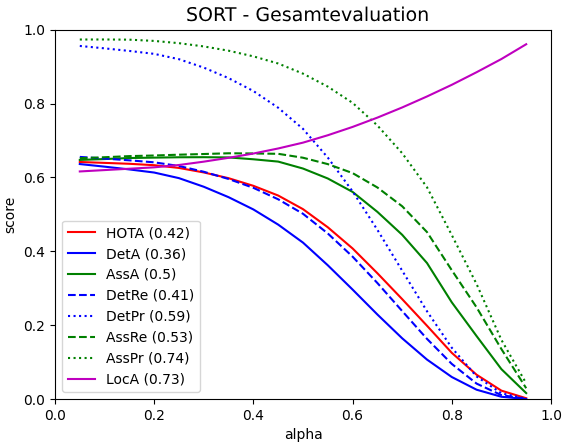
\includegraphics[width=\textwidth, height=11cm]{img/Plots/MOT Evaluation/HOTA SORT Gesamt.png}
         \caption{HOTA Gesamtevaluation des SORT Algorithmus.}
     \end{subfigure}
     \hfill
     \begin{subfigure}[b]{0.9\textwidth}
         \centering
         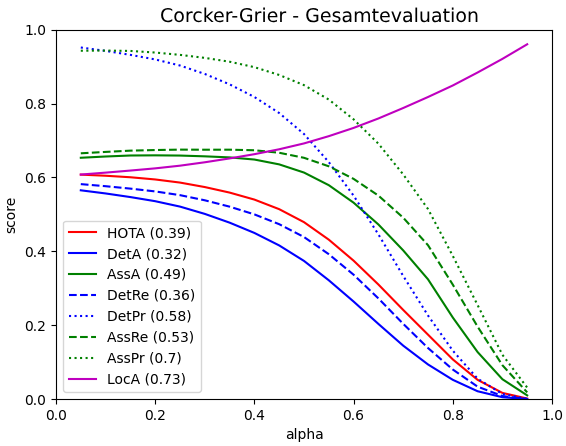
\includegraphics[width=\textwidth, height=11cm]{img/Plots/MOT Evaluation/HOTA CrockGrier Gesamt.png}
         \caption{HOTA Gesamtevaluation des Cocker-Grier Linking Algorithmus.}
     \end{subfigure}
     \caption{Verlauf der \textit{HOTA}-Wertungen der Gesamtperformance der Assoziationsalgorithmen.}
     \label{fig:ErgebGesamtMOT}
\end{figure}

\begin{table}[htbp]
\centering
\caption{Vergleich der Algorithmen mit den HOTA Matriken in \%}
\label{tab:verglHOTA}
\begin{tabular}{
  l
  S[table-format=2.3]
  S[table-format=2.3]
  S[table-format=2.3]
  S[table-format=2.3]
  S[table-format=2.3]
  S[table-format=2.3]
  S[table-format=2.3]
  S[table-format=2.3]
}
\toprule
{Algorithmus} & {HOTA} & {DetA} & {AssA} & {DetRe} & {DetPr} & {AssRe} & {AssPr} & {LocA} \\
\midrule
Cocker-Grier  & 38,797 & 31,857 & 48,526 & 35,691  & 58,362  & 52,639  & 70,188  & 72,863 \\
SORT          & 41,744 & 36,220 & 49,956 & 40,788  & 59,466  & 53,441  & 73,957  & 73,112 \\
\bottomrule
\end{tabular}
\end{table}

Zunächst ist zu bemerken, dass der prinzipielle Verlauf der Performance bei beiden Algorithmen den Erwartungen entspricht. Wie im Beispiel der Abbildung \ref{fig:MPNTrack} zu sehen ist, fallen die Wertungen mit steigendem \(\alpha\) zunehmend, während die Localisation Accuracy steigt. Es ist zu sehen, dass sich die beiden Algorithmen in ihrer Gesamtperformance stark ähneln. Insgesamt schneidet SORT leicht besser ab. Die hohe Ähnlichkeit ist darauf zurückzuführen, dass die Performance von detektionsbasierten Tracking-Systemen stark von den Detektionen beeinflusst wird. Da beide Algorithmen auf den gleichen Detektionen arbeiten, ist die ähnliche Performance nicht verwunderlich. Es ist jedoch eine Bestätigung, dass beide Algorithmen fähig sind, Assoziationen zu tätigen.\dubpar

\textbf{Diskussion der Lokalisationsbewertung}\par
Der SORT Algorithmus verwendet einen Kalman-Filter, welcher die Position der Objekte schätzt, was die Lokalisation beeinflusst. Beim Crocker-Grier Linking Algorithmus wird die Lokalisation nicht beeinflusst. Obwohl der Wert für die Lokalisationsgenauigkeit (LocA) für beide Algorithmen identisch ist, scheint dieser unterschiedliche Umgang keinen Einfluss auf die Performance zu haben.\dubpar

\textbf{Diskussion der Detektionsbewertung}\par
Auch wenn mit den gleichen Detektionen gearbeitet wurde, weisen die Detektionsmetriken Unterschiede auf. Das ist dadurch zu erklären, dass die Algorithmen an unterschiedlichen Stellen und auf unterschiedliche Weisen Detektionen aussortieren. Z.B. verwirft der modifizierte Crocker-Grier Linking Algorithmus Detektionen, wenn sie nicht verifiziert werden können. SORT lässt Detektionen unassoziiert, wenn es keine passende Assoziationen in den folgenden Frames gibt. In diesem Fall wird keine Trajektorie initialisiert. Die niedrige Bewertung des Crocker-Grier Linking Algorithmus deutet darauf hin, dass der Verifizierungsmechanismus die Detektionsqualität negativ beeinflusst. \par

Bei Betrachtung der DetRe und DetPr Wertungen ist zu sehen, dass der Crocker-Grier Linking Algorithmus sowohl mehr falsch positive Fehler macht, als auch mehr falsch negative als SORT. Eine Erklärung für die bessere Detection Precision bei SORT könnte sein, dass das Vorgehen, neue Trajektorien zu initialisieren, dafür sorgt, dass falsch positive Detektionen herausgefiltert werden. Eine andere Erklärung könnte sein, dass der Verifizierungsmechanismus des modifizierten Crocker-Grier Linking Algorithmus dafür sorgt, dass sowohl mehr richtige Detektionen verworfen werden, als auch dafür, dass mehr falsche Detektionen assoziiert werden als bei SORT. \par

\begin{wrapfigure}{l}{0.5\textwidth}
    \begin{center}
        \vspace*{-9mm}
        \begin{subfigure}[b]{0.5\textwidth}
             \centering
             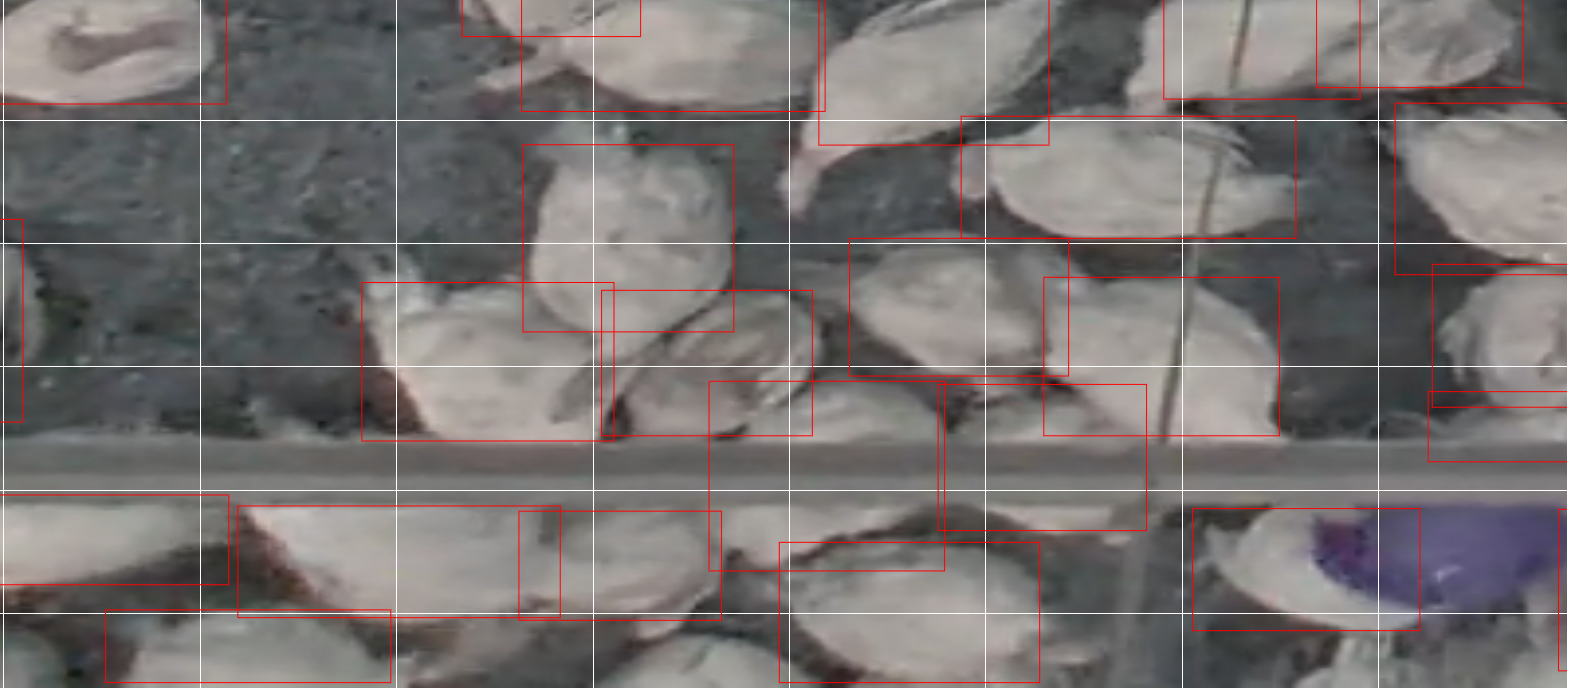
\includegraphics[width=\textwidth]{img/Vergleich GT_Track GT.png}
             \caption{Ground Truth}
         \end{subfigure}
         \hfill
         \begin{subfigure}[b]{0.5\textwidth}
             \centering         
             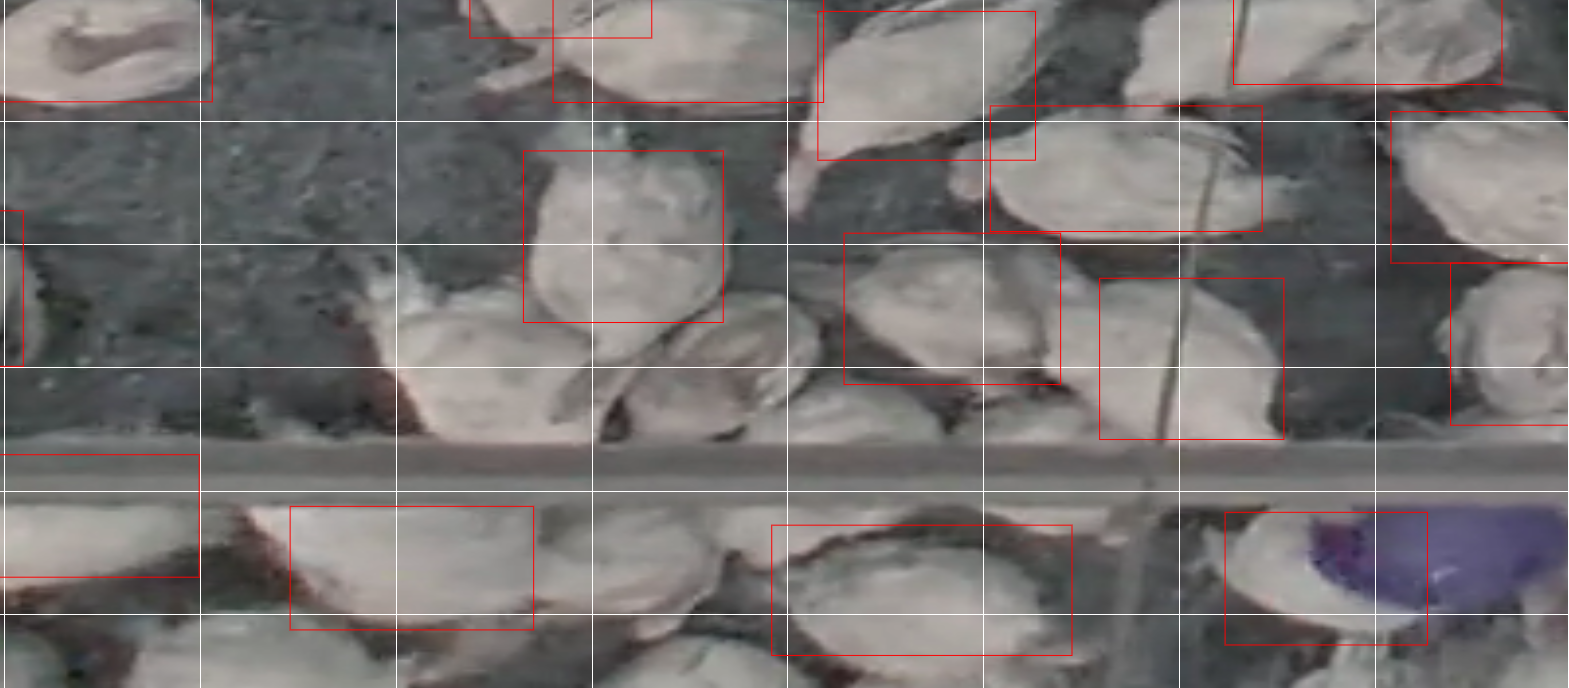
\includegraphics[width=\textwidth]{img/Vergleich GT_Track Tracking.png}
             \caption{Detektionsergebnis}
         \end{subfigure}
        \vspace*{-10mm}
        \caption{Vergleich der Ground Truth und des Detektionsmoduls.}
        \label{fig:GTvsDetsComp}
    \end{center}
\end{wrapfigure}
Bei beiden Algorithmen ist der DetRe Wert niedriger. Das bedeutet, das Detektionsmodul ist anfälliger für falsch negative Detektionen als für falsch positive. Das bedeutet, es werden nicht alle Tiere erkannt. Es ist jedoch davon auszugehen, dass die Mehrdeutigkeiten in der Ground Truth Erstellung sich negativ auf die Bewertung auswirken. Die teilweisen Verdeckungen bei den Futterbahen oder am Randbereich des Kameraausschnitts wurden in der Ground Truth strenger markiert, als es vom Detektionsmodul umgesetzt wird. Dies zeigt sich beim Vergleich der bounding Boxen in der Ground Truth und denen des Detektionsmoduls. In Abbildung \ref{fig:GTvsDetsComp} sind ausgewählte Bildbereiche miteinander verglichen. Sie stammen aus dem gleichen Frame. \par

Somit ist die Bewertung des DetRe-Werts nicht als falsch zu beurteilen, es ist jedoch zu vermuten, dass hier eine Verzerrung entsteht, da das Detektionsmodul vermutlich einen anderen Umgang mit diesen Situationen gelernt hat.\par

Das Ergebnis der Betrachtung der Detektion ist zum Vorteil von SORT. Jedoch sind die Unterschiede nur gering. Da vor allem die Trajektorienqualität entscheidend ist, sind die Assoziationsmetriken ausschlaggebender für die Entscheidung.\dubpar


\textbf{Diskussion der Assoziationsbewertung}\par
Bezogen auf die \textit{HOTA}-Metrik und die DetA-Wertung ist zu sehen, dass das Assoziationsmodul besser abschneidet als das Detektionsmodul. Das ist vorteilhaft, da vor allem die Trajektorienqualität für die Anwendung wichtig ist. Die AssA-Wertung bleibt deutlich länger konstant und wird kaum von \(\alpha\) beeinflusst. \par

Auch hier schneidet SORT besser ab. Während der AssRe-Wert bei beiden Algorithmen gleich ist, unterscheidet sich der AssPr-Wert deutlich. Der  Crocker-Grier Linking Algorithmus ist anfälliger für Merging-Fehler als SORT. Insgesamt ist der AssRe Wert jedoch niedriger als der AssPr-Wert. Das bedeutet, dass beide Algorithmen anfälliger für Fragmentationen als für Merging-Fehler sind.\par

Insgesamt sind die AssRe-Wertung und die AssPr-Wertung als gut zu bewerten. Sie fallen relativ schnell mit steigendem \(\alpha\), jedoch sind sie sehr hoch. Die Fehleranzahl ist also insgesamt niedrig. Das lässt vermuten, dass die Algorithmen Trajektorien generieren können, aus denen sich aussagekräftige Features extrahieren lassen.\dubpar

\textbf{Präsentation der Metriken}

Die Tabelle \ref{tab:MOTgesamtÜbersicht} zeigt eine Übersicht der beiden Algorithmen mit den unterschiedlichen Metriken.

\begin{table}[htbp]
\centering
\caption{Übersicht über die Metriken zu der Beurteilung der Gesamtperformance.}
\label{tab:MOTgesamtÜbersicht}
\begin{tabular}{
  l
  S[table-format=2.3]
  S[table-format=2.3]
  S[table-format=2.3]
  S[table-format=2.3]
  S[table-format=2.3]
}
\toprule
{Algorithmen} & {HOTA} & {MOTA} & {MOTP} & {MODA} & {IDF1} \\
\midrule
Crocker-Grier & 38,797 & 26,278 & 69,156 & 27,103 & 47,870 \\
SORT          & 41,744 & 31,095 & 69,391 & 32,032 & 52,371 \\
\bottomrule
\end{tabular}
\end{table}

\textbf{Fazit}

Die Algorithmen sind in ihrer Performance ähnlich. Insgesamt ist SORT etwas besser. Die Assoziationsqualität verspricht Trajektorien zu genieren, aus denen sich aussagekräftige Features extrahieren lassen. 


\subsection{Analyse der Abhängigkeit der Performance von der Verhaltensweise}
Es sind zwei Ground Truths vorhanden. Eine beinhaltet ein Kampfereignis und die andere einen Kontrollgang. Nach menschlicher Beurteilung besteht der Verdacht, dass die Assoziationsalgorithmen bei höherer Dynamik schlechter performen. Dieser Verdacht wird untersucht. Das Kampfereignis weist deutlich weniger Dynamik auf, als der Kontrollgang.\par

Die Abbildung \ref{fig:SORTHOTAEREIG} zeigt die Verläufe der \textit{HOTA}-Metriken zum SORT Algorithmus, wobei die Bewertung beider Ereignisse dargestellt ist. Abbildung \ref{fig:CROCKHOTAEreig} zeigt dies für die Bewertung des Crocker-Grier Linking Algorithmus. Die Tabelle \ref{tab:HOTAübersEreig} zeigt eine Übersicht über die Ergebnisse.

\begin{figure}[htbp]
     \centering
     \begin{subfigure}[b]{0.9\textwidth}
         \centering
         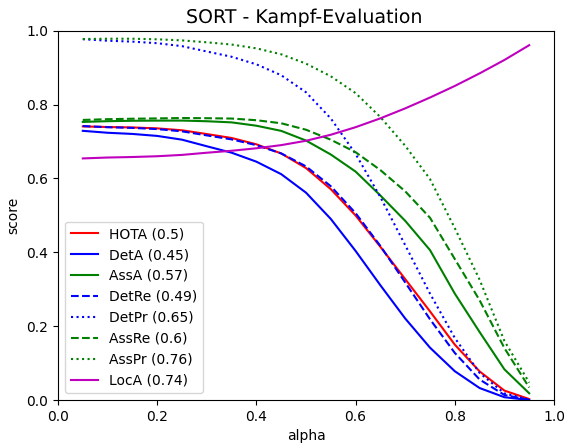
\includegraphics[width=\textwidth, height=11cm]{img/Plots/MOT Evaluation/HOTA SORT Kampf.png}
         \caption{Evaluation mit dem Kampfereignis.}
     \end{subfigure}
     \hfill
     \begin{subfigure}[b]{0.9\textwidth}
         \centering
         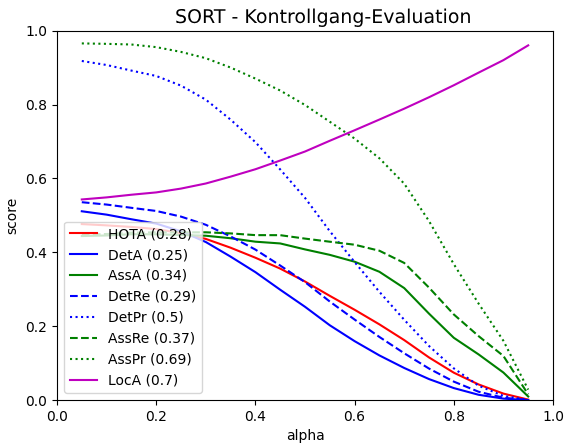
\includegraphics[width=\textwidth, height=11cm]{img/Plots/MOT Evaluation/HOTA SORT Kontrollgang.png}
         \caption{Evaluation mit dem Kontrollgang.}
     \end{subfigure}
     \caption{Evaluation des SORT Algorithmus in Bezug auf die Verhaltensweise.}
     \label{fig:SORTHOTAEREIG}
\end{figure}

\begin{figure}[htbp]
     \centering
     \begin{subfigure}[b]{0.9\textwidth}
         \centering
         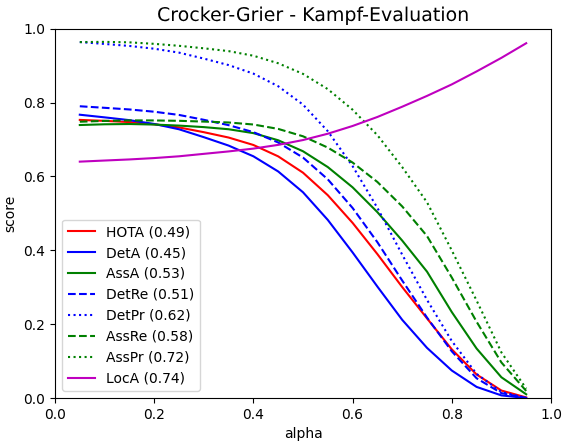
\includegraphics[width=\textwidth, height=11cm]{img/Plots/MOT Evaluation/HOTA CrockGrier Kampf.png}
         \caption{Evaluation mit dem Kampfereignis.}
     \end{subfigure}
     \hfill
     \begin{subfigure}[b]{0.9\textwidth}
         \centering
         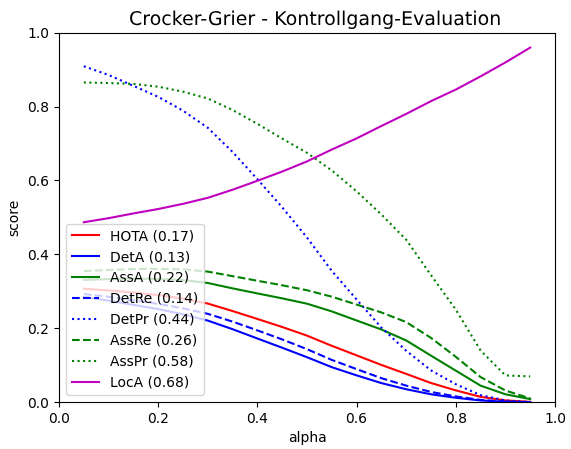
\includegraphics[width=\textwidth, height=11cm]{img/Plots/MOT Evaluation/HOTA CrockGrier Kontrollgang.png}
         \caption{Evaluation mit dem Kontrollgang.}
     \end{subfigure}
     \caption{Evaluation des Crocker-Grier Linking Algorithmus in Bezug auf die Verhaltensweise.}
     \label{fig:CROCKHOTAEreig}
\end{figure}

\begin{table}[htbp]
\centering
\caption{Performance der Algorithmen in Bezug auf das Ereignis.}
\label{tab:HOTAübersEreig}
\begin{tabular}{
  l
  l
  S[table-format=2.2]
  S[table-format=2.2]
  S[table-format=2.2]
  S[table-format=2.2]
  S[table-format=2.2]
  S[table-format=2.2]
  S[table-format=2.2]
  S[table-format=2.2]
}
\toprule
{Algorithmus} & {Ereignis} & {HOTA} & {DetA} & {AssA} & {DetRe} & {DetPr} & {AssRe} & {AssPr} & {LocA} \\
\midrule
SORT          & Kampf      & 49,53 & 44,50 & 56,63 & 49,10  & 64,65  & 60,28  & 75,64  & 74,49 \\
SORT          & Kontrollgang & 28,37 & 25,43 & 33,73 & 29,22  & 50,07  & 36,66  & 69,09  & 70,20 \\
Crocker-Grier & Kampf      & 48,67 & 45,28 & 53,40 & 51,12  & 62,36  & 57,53  & 72,08  & 73,97 \\
Crocker-Grier & Kontrollgang & 28,37 & 25,43 & 33,73 & 29,22  & 50,07  & 36,66  & 69,09  & 70,20 \\
\bottomrule
\end{tabular}
\end{table}

\textbf{Diskussion zum Kampfereignis}\par
Im Vergleich zur Gesamtperformance ist das MOT System besser, wenn es nur mit dem Kampfereignis beurteilt wird. Die grundlegenden Trends bleiben erhalten, wobei SORT in den meisten Metriken besser abschneidet als der Crocker-Grier Linking Algorithmus. Im Vergleich zur Gesamtperformance bleiben die Werte länger konstant, wenn \(\alpha\) steigt. \par

Der Crocker-Grier Linking Algorithmus weist hier einen besseren DetRe-Wert als SORT auf. Das ist damit zu erklären, dass der Verifizierungsmechanismus vermutlich einen Großteil der Trajektorien verifizieren kann. Dadurch bleiben wenige Detektionen ungenutzt. SORT hingegen verwirft offenbar einige echt positive Detektionen, da sie zu keiner Trajektorie initialisiert werden können. Da die restlichen Wertungen des Crocker-Grier Linking Algorithmus jedoch niedriger sind, scheint die erhöhte Menge verifizierter Trajektorien sich nicht positiv auf die Ergebnisse des Systems auszuwirken.\dubpar  


\textbf{Diskussion zum Kontrollgang}\par
Die Performance im Kontrollgang sinkt erheblich. Die Ergebnisse bestätigen den menschlichen Eindruck, dass die Qualität bei erhöhter Dynamik sinkt. Alle Fehlerarten nehmen zu und jede Wertung sinkt im Vergleich zum Kampfereignis. \par

Hier zeigt sich ein deutlicherer Unterschied zwischen den Algorithmen. Der Performanceverlust vom Crocker-Grier Linking Algorithmus ist höher als der von SORT, und das gilt für sämtliche Metriken. Da vor allem die Korrektheit der Trajektorien wichtig ist, um Features zu extrahieren, sind die Assoziationswertungen am relevantesten. SORT ist der Algorithmus, welcher bei höherer Dynamik die richtigeren Trajektorien generiert.\par

Der AssRe-Wert zeigt, dass sich im Kontrollgang Fragmentation häuft. Das kann für die Extraktion von Features problematisch werden. Sind Bewegungen zu stark fragmentiert, spiegeln die Trajektorien eventuell wichtige Merkmale der Bewegung nicht wider. Findet die Fragmentation bspw. immer dann statt, wenn eine explosive Geschwindigkeitserhöhung stattfindet, können die Features, die aus diesen Trajektorien extrahiert werden, die Dynamik des Geschehens nicht abbilden. In der Feature-Auswahl ist zu untersuchen, ob sich mit den extrahierten Features ein Kontrollgang von den anderen Verhaltensweisen unterscheiden lässt. Die Assoziationswertungen des SORT Algorithmus sind jedoch in der Hinsicht vielversprechend, da auch bei hoher Dynamik richtige Trajektorien generiert werden. Ob diese das Geschehen korrekt repräsentierten, muss über die Features untersucht werden.\dubpar


\textbf{Präsentation der Metriken}\par

In Tabelle \ref{tab:MetrikenEregins} sind die unterschiedlichen Metriken im Vergleich dargestellt. Angegeben sind sie zu jedem Ereignis und jedem Algorithmus.

\begin{table}[htbp]
\centering
\caption{Übersicht über die Metriken zu der Bewertung der Ereignisse.}
\label{tab:MetrikenEregins}
\begin{tabular}{
  l
  l
  S[table-format=2.3]
  S[table-format=2.3]
  S[table-format=2.3]
  S[table-format=2.3]
  S[table-format=2.3]
}
\toprule
{Algorithmus} & {Ereignis} & {HOTA} & {MOTA} & {MOTP} & {MODA} & {IDF1} \\
\midrule
SORT          & Kampf      & 49,537 & 50,229 & 70,168 & 50,951 & 65,288 \\
SORT          & Kontrollgang & 28,379 & 4,4885 & 67,252 & 5,722 & 32,415 \\
Crocker-Grier & Kampf      & 48,673 & 48,019 & 69,801 & 48,967 & 63,813 \\
Crocker-Grier & Kontrollgang & 28,379 & 4,4885 & 67,252 & 5,722 & 32,415 \\
\bottomrule
\end{tabular}
\end{table}

\textbf{Fazit}\par
Insgesamt hängt die Performance stark von den Ereignissen und der Dynamik ab. Das Trackingergebnis ist bei hoher Dynamik deutlich schlechter. Gerade bei hoher Dynamik erzeilt der SORT Algorithmus eine deutlich bessere Performance als der Crocker-Grier Linking Algorithmus. Korrekte Trajektorien werden in beiden Ereignissen generiert. In der Feature-Auswahl ist zu überprüfen, ob die extrahierten Features einen Kontrollgang so repräsentieren, dass er sich von den anderen Verhaltensweisen unterscheiden lässt.


\subsection{Vergleich und Auswertung der Laufzeiten}
Die Laufzeiten der beiden Algorithmen sind für unterschiedliche Ereignislängen ermittelt worden. In der Abbildung \ref{fig:plotRunTMOT} sind die Laufzeiten in Abhängigkeit der Ereignisdauer geplottet.

\begin{figure}[htb]
    \centering
    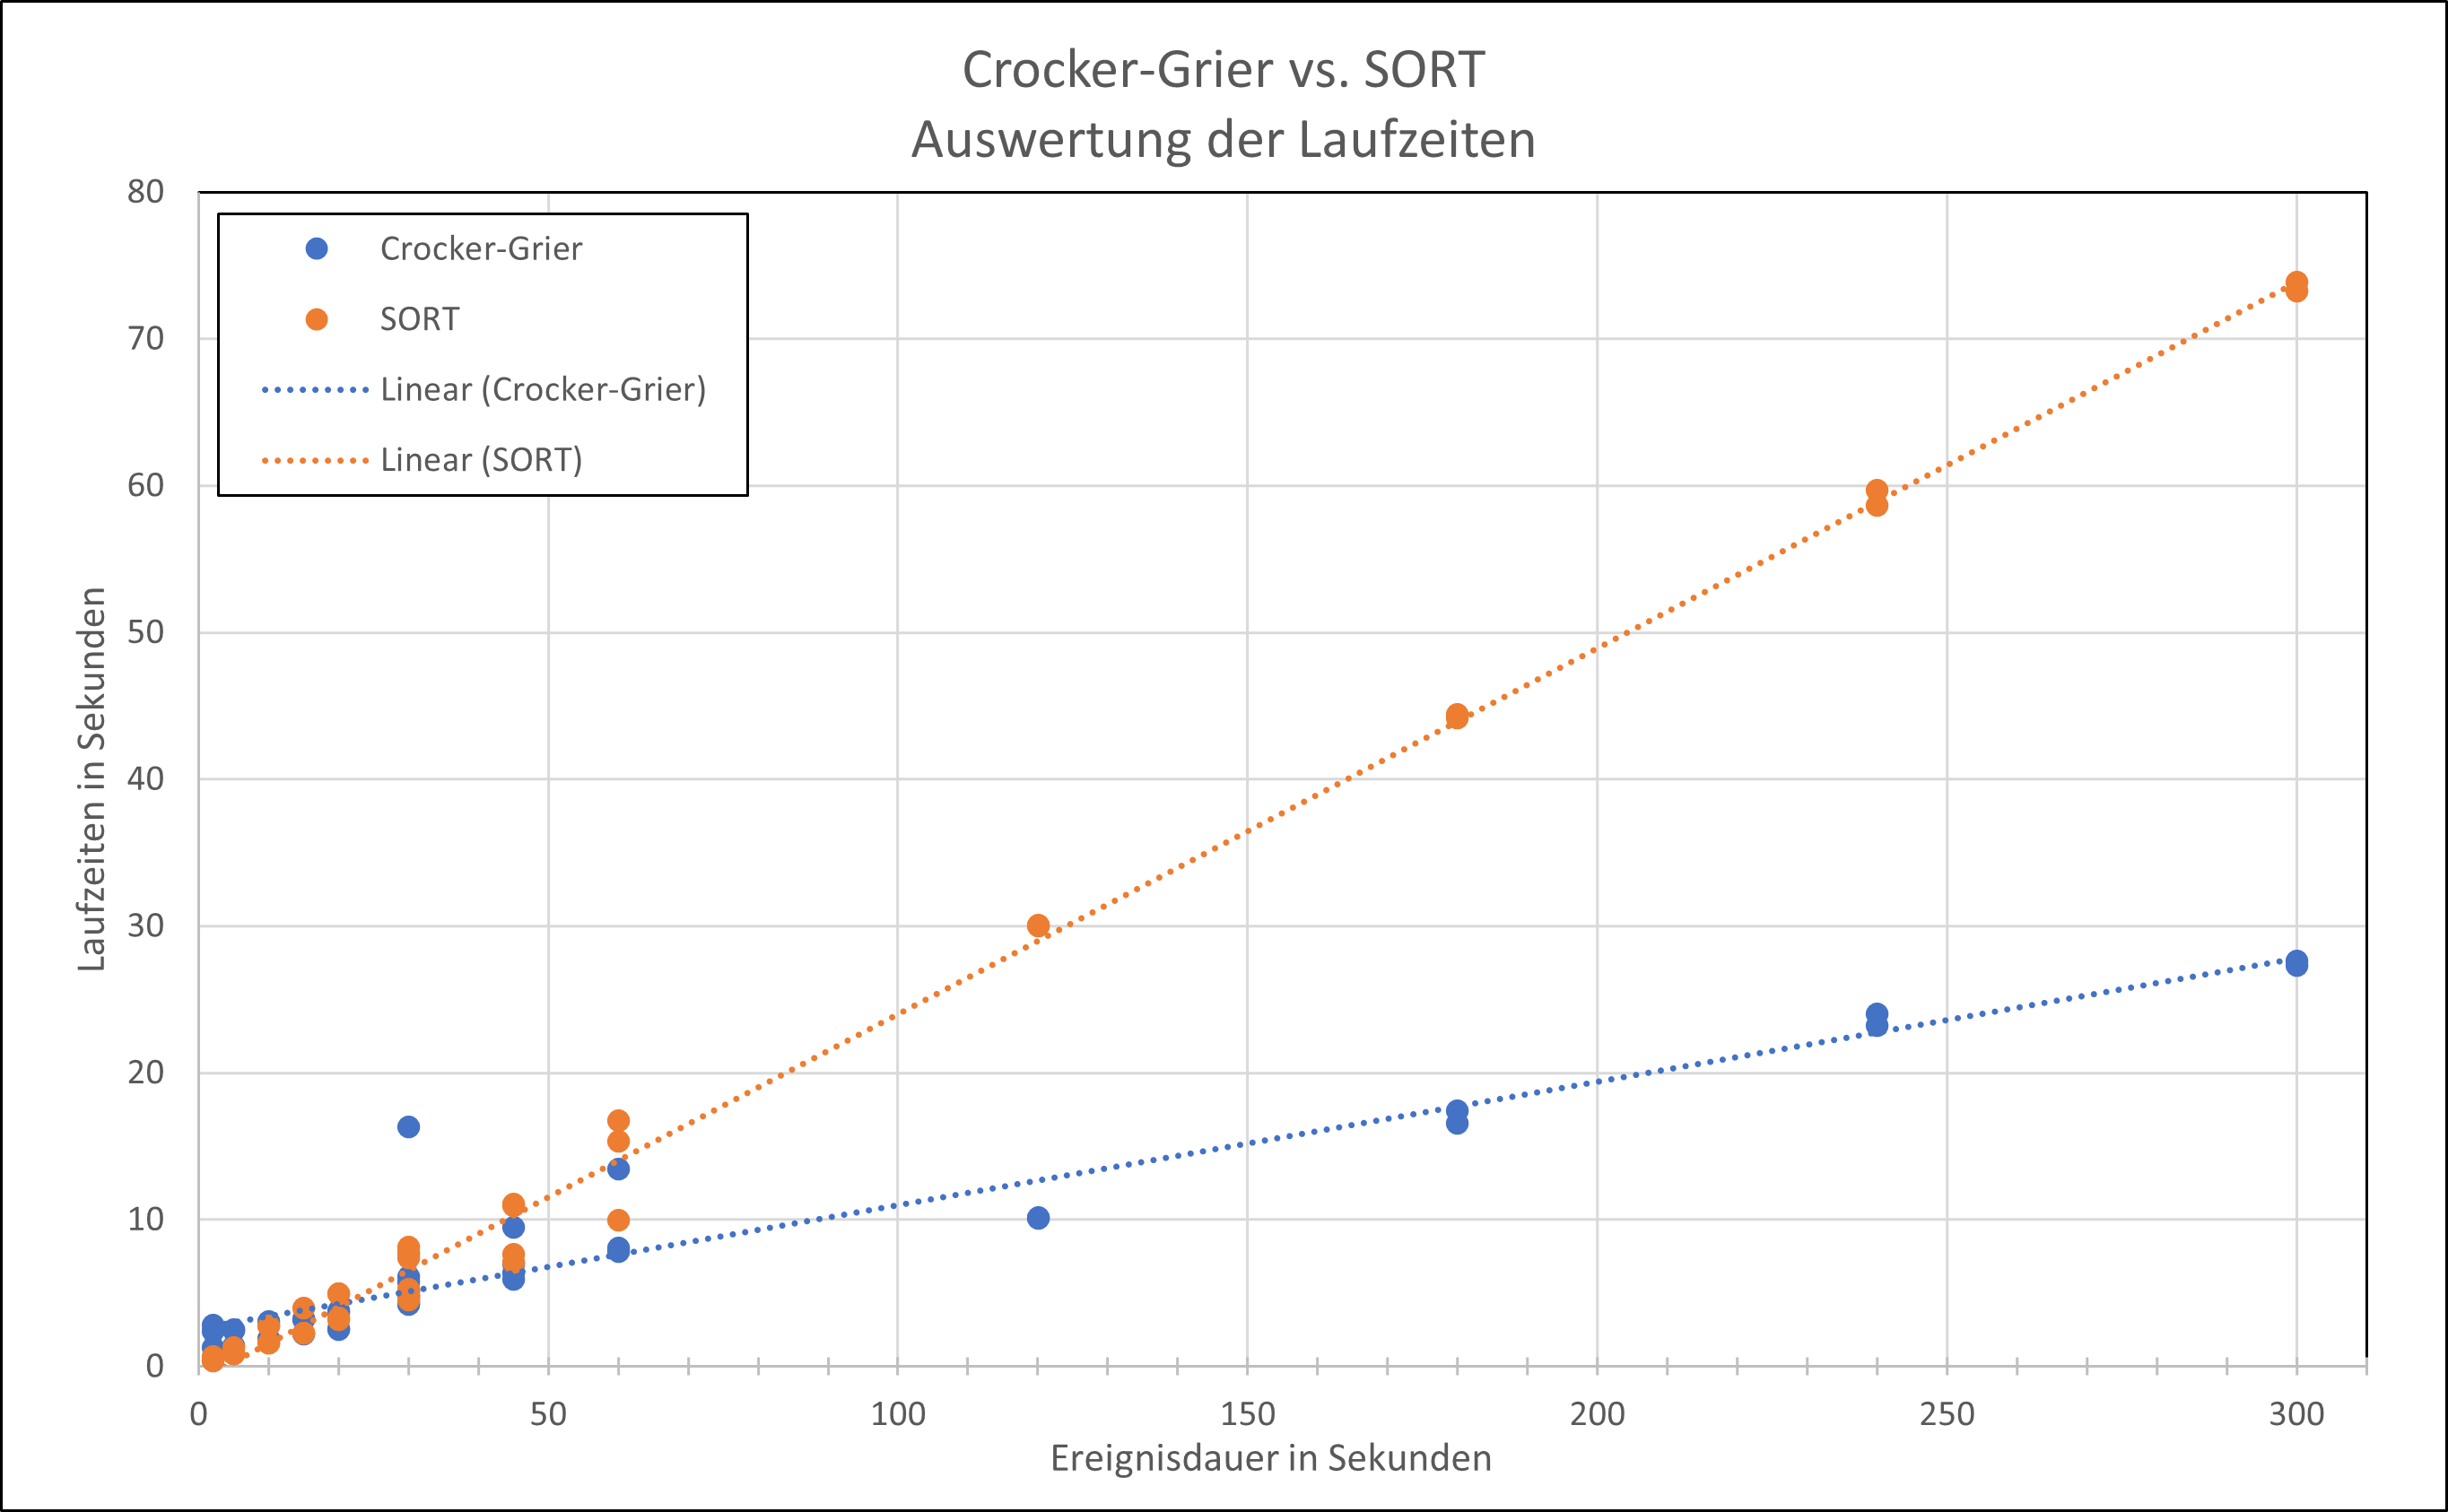
\includegraphics[width=0.9\textwidth]{img/Plots/MOT Evaluation/Assoziationsalgorithmen Laufzeiten.png}  
    \caption{Laufzeiten der Assoziation in Abhängigkeit der Ereignisdauer.}
    \label{fig:plotRunTMOT}
\end{figure}

Es ist zu sehen, dass der Crocker-Grier Linking Algorithmus besser skaliert, jedoch weist er ein klein bisschen mehr Overhead auf. Durch den Overhead ist der zeitliche Vorteil für kleine Ereignislängen von weniger als 30 Sekunden nicht signifikant. Die Trendlinien beider Algorithmen zeigen, dass die Laufzeiten für Ereignisse, die kürzer als 5 Minuten sind, annähernd linear skalieren. Da Beide Trendlinien eine Steigung kleiner eins aufweisen, erfüllen sie die Grundvoraussetzung für die Anwendung im Modul. Andernfalls könnte keine lückenlose Abtastung des Stallgeschehens erfolgen. Nach der Auswahl einer Intervallgröße für die Ereignisse kann über die zeitliche Skalierung der Laufzeit eingeschätzt werden, wie viel Zeit die restliche Verarbeitung in Anspruch nehmen darf, um eine lückenlose Abtastung zu erreichen.  \dubpar

\textbf{Fazit}\par
Die Laufzeit des Crocker-Grier Linking Algorithmus skaliert etwas besser. Für kurze Ereignisse ist der Unterschied jedoch vernachlässigbar. Mit beiden Algorithmen kann eine lückenlose Abtastung des Stallgeschehens erreicht werden.

\subsection{Fazit der Analysen zum MOT System}
Für das Modul wird der SORT Algorithmus verwendet, da er in fast allen Belangen besser performt als der Crocker-Grier Linking Algorithmus. Ausschlaggebend ist die erheblich bessere Performance in hochdynamischen Ereignissen. In solchen Ereignissen besteht die Gefahr, dass die Features, die aus den Trajektorien extrahiert werden, das dynamische Geschehen nicht korrekt repräsentieren. Dies ist zu untersuchen. Insgesamt sind jedoch korrekte Assoziationen in jedem Ereignis zu erwarten. Die Laufzeiten der Algorithmen beeinflussen die Entscheidung zwischen den Algorithmen nicht, da beide die Kriterien in Bezug auf die Laufzeit erfüllen, um im Modul angewendet zu werden.
\section{Feature-Auswahl, Hyperparametersuche und Modellauswahl} \label{sec:Ergeb FeatSel,Hyp,ModSel}
Um eine optimale Feature-Menge zu finden, wird aus einer Reihe von Versuchen mit Wrapper-Methoden eine Feature-Rangfolge abgeleitet. Um die Feature-Menge unabhängig vom Modell zu beurteilen, wird die Accuracy von mehreren Modellen validiert und anschließend gemittelt. In diesem Kapitel werden die Feature-Rangfolgen der Filter-Methoden betrachtet. Damit wird die konstruierte Rangfolge aus dem Wrapper-Score verglichen. Es wird untersucht, ob sich das Entfernen von Features, die auf dem gleichen Basis-Feature aufbauen, positive auswirkt. Ebenfalls wird untersucht, ob alle Feature-Kategorien benötigt werden. Abschließen tut das Kapitel mit dem Vergleich der betrachteten Modelle und dem finalen Test des ausgewählten Modells.\par

Ziel der Untersuchung ist es, für das Modul das bestmögliche Modell zu schaffen. Zu suchen ist eine Feature-Menge und ein Modell, welche besser performen, als andere Feature-Mengen oder Modelle. Zu berücksichtigen ist die Verarbeitungszeit. Für das Modul ist eine kleine Feature-Menge vorteilhafter für die Echtzeitfunktionalität. \par


\subsection{Vergleich der Filter-Methoden mit der entworfenen Rangfolge}
Die Plots in der Abbildung \ref{fig:plotMethVergl} zeigen den Verlauf der Accuracy in Bezug zur Feature-Menge gemäß der jeweiligen Rangfolge. Dargestellt sind die Varianzanalyse, die gegenseitige Information und der Wrapper-Score. Zur besseren Vergleichbarkeit sind die Sättigungskurve eingezeichnet. Die Tabelle \ref{tab:FiltVsWrap} zeigt einen tabellarischen Vergleich.

\emptyFigure{Verlauf der Accuracy der Filter-Methoden und der entworfenen Rangfolge.}{fig:plotMethVergl}
\todo{Abbildung fehlt}

\begin{table}[htbp]
\centering
\caption{Vergleich der Sättigungspunkte der Rangfolgen.}
\label{tab:FiltVsWrap}
\begin{tabular}{
  >{\raggedright\arraybackslash}p{0.4\linewidth}
  S[table-format=2.0]
  S[table-format=3.0]
}
\toprule
{Methode} & {Accuracy [\%]} & {Featureanzahl} \\
\midrule
Varianzanalyse & 82 & 48 \\
gegenseitige Information & 83 & 112 \\
Wrapper-Score & 85 & 36 \\
\bottomrule
\end{tabular}
\end{table}

Es ist zu sehen, dass die Rangfolge nach dem Wrapper-Score im besten Verlauf der Accuracy resultiert. Die Sättigung wird mit der kleinsten Feature-Menge erreicht und die Accuracy ist im Vergleich am höchsten. Das legitimiert das Vorgehen. \par

Wie in \ref{sec:Meth KonstrFeatures} dargestellt, liegt die Feature-Anzahl bei 3114. Die Plots zeigen, dass nur ein Bruchteil dieser Menge notwendig ist, um die Sättigung zu erreichen. Das spricht für viel Redundanz in den Features.


\subsection{Auswirkungen der Entfernung von Features gleicher Basis}
Die Rangfolgen werden bearbeitet. Von den Features, die auf dem gleichen Basis-Feature aufbauen, befindet sich schließlich nur noch das Höchstrangige in der Rangfolge. Dadurch soll Redundanz reduziert werden. In der Abbildung \ref{fig:plotRIPsame Bais} sind die entsprechenden Plots zu den Rangfolgen der Filter-Methoden und des Wrapper-Scores zu sehen und in der Tabelle \ref{tab:entfSameBasis} befindet sich ein tabellarischer Vergleich.

\emptyFigure{Verlauf der Accuracy nach dem Entfernen von Features mit gleicher Basis.}{fig:plotRIPsame Bais}
\todo{Abbildung fehlt}

\begin{table}[htbp]
\centering
\caption{Vergleich der Sättigungspunkte nach entfernen von Features gleicher Basis.}
\label{tab:entfSameBasis}
\begin{tabular}{
  >{\raggedright\arraybackslash}p{0.4\linewidth}
  S[table-format=2.0]
  S[table-format=3.0]
}
\toprule
{Methode} & {Accuracy [\%]} & {Featureanzahl} \\
\midrule
Varianzanalyse & 83 & 44 \\
gegenseitige Information & 83 & 63 \\
Wrapper-Score & 86 & 34 \\
\bottomrule
\end{tabular}
\end{table}

Es ist zu sehen, dass sich das Entfernen von Features, mit gleicher Basis, auf alle Feature-Rangfolgen positiv ausgewirkt. Es wird eine bessere Accuracy mit weniger Features erreicht. Somit lässt sich sagen, dass tatsächlich Redundanzen entfernt werden, wodurch eine Feature-Menge entsteht, welche dem Modell mehr Information bietet als zuvor.


\subsection{Performancevergleich der Feature-Kategorien}
Aus der Rangfolge des Wrapper-Scores werden nur bestimmte Feature-Kategorien und Kombinationen von Kategorien getestet. Die Verläufe der Accuracy sind in der Abbildung \ref{fig:plotCompKateg} zu sehen. Eine tabellarische Darstellung befindet sich in der Tabelle \ref{tab:comKate}.

\emptyFigure{Verlauf der Accuracy von unterschiedlichen Kombinationen der Feature-Kategorien.}{fig:plotCompKateg}
\todo{Abbildung fehlt}

\begin{table}[htbp]
\centering
\caption{Vergleich der Sättigungspunkte unterschiedlicher Kategorie-Kombinationen}
\label{tab:comKate}
\begin{tabular}{
  >{\raggedright\arraybackslash}p{0.5\linewidth}
  S[table-format=2.0]
  S[table-format=2.0]
}
\toprule
{Kombination} & {Accuracy [\%]} & {Featureanzahl} \\
\midrule
Basis & 81 & 11 \\
Interaktion & 85 & 9 \\
Quantil & 84 & 11 \\
Log & 82 & 16 \\
BoxCox & 81 & 14 \\
\midrule
Basis-Interaktion & 85 & 28 \\
Basis-Quantil & 83 & 15 \\
Basis-Log & 82 & 16 \\
Basis-BoxCox & 82 & 13 \\
\midrule
Basis-Interaktion-Quantil & 86 & 29 \\
Basis-Interaktion-Log & 85 & 20 \\
Basis-Interaktion-BoxCox & 85 & 28 \\
Basis-Quantil-Log & 83 & 14 \\
Basis-Quantil-BoxCox & 83 & 15 \\
Basis-Log-BoxCox & 82 & 14 \\
\midrule
Basis-Interaktion-Quantil-Log & 86 & 28 \\
Basis-Interaktion-Quantil-BoxCox & 85 & 30 \\
Basis-Interaktion-Log-BoxCox & 85 & 31 \\
Basis-Quantil-Log-BoxCox & 84 & 20 \\
\midrule
Basis-Interaktion-Quantil-Log-BoxCox & 85 & 30 \\
\bottomrule
\end{tabular}
\end{table}

Es ist zu sehen, dass die höchste Accuracy mit der Kombination aus den Basis-Features, den Interaktionsfeatures und den Quantil-Features erreicht wird, oder mit der gleichen Kombination, mit den logarithmischen Features zusätzlich. Im zweiten Fall wird die Sättigung mit einem Feature weniger erreicht. Um die Berechnung der logarithmischen Features einzusparen, wird sich für die erste Kombination entschieden.\par

Die Box-Cox-Features und die logarithmischen Features werden nicht verwendet für das Modul.


\subsection{Untersuchungen zur Modellauswahl} \label{sec:ErgebModSelEval}
Die Abbildung \ref{fig:plotCompModel} zeigt die Plots der Accuracy zu den unterschiedlichen Modellen. In der Tabelle \ref{tab:compModel} ist der Vergleich der Sättigungspunkte zu sehen.

\emptyFigure{Verlauf der Accuracy der unterschiedlichen Modelle.}{fig:plotCompModel}
\todo{Abbildung fehlt}

\begin{table}[htbp]
\centering
\caption{Vergleich der verschiedenen Modelle}
\label{tab:compModel}
\begin{tabular}{
  >{\raggedright\arraybackslash}p{0.5\linewidth}
  S[table-format=2.0]
  S[table-format=2.0]
}
\toprule
{Modelle} & {Accuracy [\%]} & {Featureanzahl} \\
\midrule
logistische Regression & 86 & 10 \\
lineare SVM & 87 & 24 \\
polynomiale SVM & 87 & 18 \\
Random Forest & 85 & 18 \\
Histografisches Gradient Boosting & 86 & 21 \\
\bottomrule
\end{tabular}
\end{table}

Es ist zu sehen, dass Unterschiede in der Performance zwischen den Modellen, nach der Hyperparametersuche kaum vorhanden sind. Die niedrigste Feature-Anzahl benötigt die logistische Regression. Bei Betrachtung der Abbildung \ref{fig:plotCompModel} wirkt es jedoch so, dass die Sättigungskurve hier den Verlauf nicht richtig approximiert. Der tatsächliche Sättigungspunkt wird ebenfalls bei ca. 20 Features erreicht. Am besten schneiden die SVMs ab. Die polynomiale SVM erreicht die Sättigung mit einer etwas kleineren Feature-Anzahl als die lineare SVM. Aus diesem Grund fällt die Entscheidung auf die polynomiale SVM.

Die Abbildung \ref{fig:plotTrainTestFinal} zeigt den Vergleich der Accuracy des Trainings, der Validierung und des Testens. Es ist zu sehen, dass die Wertungen nah aneinander verlaufen. Dadurch ist auszuschließen, dass das Modell overfittet. Dass der Trainingswert etwas besser ist, als der Validierungswert und der Testwert ist üblich und zu erwarten. 

\emptyFigure{Verlauf der Accuracy des Trainings, der Validierung und des Testens des finalen Modells.}{fig:plotTrainTestFinal}
\todo{Abbildung fehlt}

Die Abbildung \ref{fig:KonfMatr} zeigt die Konfusionsmatrix des finalen Tests.

\emptyFigure{Konfusionsmatrix des Testens des finalen Modells.}{fig:KonfMatr}
\todo{Abbildung fehlt}

\subsection{Fazit der Untersuchungen zur Feature-Auswahl und der Modellauswahl}
Die Ermittlung der Feature-Rangfolge über den Wrapper-Score übertrifft die der Filter-Methoden. Dadurch ist bestätigt, dass multivariate Einflüsse Modell unabhängig berücksichtigt werden. Das Entfernen von Features, die sich die Basis teilen, reduziert Redundanz und verbesser die Feature-Rangfolge. Für eine gute Performance ist es ausreichend nur die Basis-Features, die Quantil-Features und die Interaktionsfeatures zu ermitteln. Mit dieser Rangfolge und den eingestellten Hyperparametern sind nur kleine Unterschiede in der Performance der Modelle festzustellen. Mit der polynomialen SVM lässt sich laut den Daten die beste Accuracy mit der kleinsten Feature-Anzahl erreichen. Dieses Modell wird ausgewählt. Um stabiler in der Sättigung zu liegen wird die Feature-Anzahl auf 40 vergrößert.
\section{Machbarkeit der Echtzeit-Verhaltensklassifizierung} \label{sec:Ergeb Sim}
Um zu bestätigen, dass eine Echtzeit-Verhaltensklassifizierung umsetzbar ist, muss die Funktionalität des Moduls verifiziert werden. Dazu ist zu untersuchen, ob die Anforderungen erfüllt werden. In diesem Kapitel wird die Anwendungssimulation ausgewertet, um diese Fragen zu beantworten. \par

Überprüft wird, die lückenlose Abtastung des Stallgeschehens und Echtzeitfähigkeit. Dazu findet eine Betrachtung der Laufzeiten statt. Auch die Abtastrate des Moduls wird ermittelt. Der größte Fokus liegt auf der Korrektheit der Schätzung. Es wird untersucht, ob das Modul dazu in der Lage, das Verhalten in der Anwendung korrekt zu bestimmen. \par

Die Simulation wird zweimal durchgeführt, mit jeweils unterschiedlichen Daten. Der erste Durchlauf betrachtet Daten aus einem Kamerabereich, der auch in den Trainingsdaten vorhanden ist. Der zweite Durchlauf betrachtet Daten aus einem zuvor nicht genutzten Kamerabereich. Alle Daten stammen aus dem ersten Mastdurchlauf. Es wird immer ein kompletter Aufzeichnungstag durchlaufen. Das Modul misst während der Verarbeitung die Laufzeiten automatisch. \par

Die Auswertung der erfolgt manuell. Die Videos zu den ausgewählten Daten werden angesehen und dabei werden die Verhaltensweisen notiert. Dadurch entsteht ein Datensatz, welcher als Referenz verwendet wird. Aus dem Ergebnis des Moduls werden die erkannten Kontrollgänge und Kämpfe nochmal gesondert betrachtet, um sicherzugehen, dass die erkannte Verhaltensweise beim Erstellen der Referenz nicht übersehen wurde.\par

\subsection{Auswertung der Laufzeiten}

Die Abbildung \ref{fig:HistGesamt} zeigt ein Histogramm der Gesamtlaufzeiten der Verarbeitung des Moduls.  

\emptyFigure{Histogramm der Gesamtlaufzeiten der Verarbeitung.}{fig:HistGesamt}
\todo{Abbildung fehlt}

Im Mittel benötigt die Verarbeitung 4,14 Sekunden. Mittelwert und Median liegen dicht bei einander. Die maximale gemessene Verarbeitungsdauer beträgt 5,23 Sekunden. Diese Werte bestätigen, dass eine lückenlose Abtastung des Stallgeschehens realisiert ist. Im Schnitt überlappen die Intervalle fast 36 Sekunden. Das sollte in einer geringen Diskrepanz zwischen dem Auftreten eines Ereignisses und der Erkennung resultieren. Die Verarbeitungszeit bestimmt die Abtastrate des Moduls. Es wird somit alle 4,14 Sekunden abgetastet. \par

Mit diesem Wissen lässt sich die minimale und maximale Dauer bestimmen, die es benötigt, ein Ereignis zu erkennen. Durch die Vorgaben, dass ein Intervall 40 Sekunden umfasst und dass ein Ereignis 30 Sekunden davon einnehmen muss, um erkannt zu werden, lässt sich der Ausdruck in \ref{eq:deltTErkenn} formulieren. \(D\) ist die Laufzeit des Ereignisses bei einem Abtastzeitpunkt und \(T\) ist die Dauer der Verarbeitung. Läuft das Ereignis exakt 30 Sekunden, umfasst es die Minimalanforderung, um erkannt zu werden. In diesem Fall wird das Ereignis so früh wie für das Modul möglich erkannt. Fällt die Abtastung so, dass das Ereignis gerade so keine 30 Sekunden umfasst, dann resultiert dies in der maximalen Erkennungsdauer. Ausgehend von der maximalen und minimalen Verarbeitungsdauer des Moduls, wird ein Ereignis frühstens nach 33,33 Sekunden erkannt und spätestens nach 40,46 Sekunden.

\begin{equation}
    \label{eq:deltTErkenn}
    \text{Gesamtzeit} = 
    \begin{cases} 
    30 + T & \text{Minimum (} D = 30 \text{ Sekunden)} \\
    D + 2T & \text{Maximum (} D < 30 \text{ Sekunden, nahe an 30)}
    \end{cases}
\end{equation}

 Echtzeitfähigkeit bedeutet, dass ein System innerhalb einer festgelegten Zeitspanne auf den Eingang reagiert. Das Ergebnis muss nach einer vorgegebenen Dauer feststehen \cite{Scholz.2005}. Für das Modul sind im Vorfeld keine harten Zeitschranken definiert worden, die einzuhalten sind. Jedoch ist über die Anforderung der lückenlose Abtastung indirekt eine Vorgabe an die Verarbeitungszeit formuliert. Die Dauer der Ermittelung des Ergebnisses muss kürzer sein, als der Ereignisintervall. Da diese Anforderung erfüllt wird, ist das Modul, als Echtzeitfähig zu bewerten. 


\subsection{Evaluation der Verhaltensklassifikation}
Die Abbildung \ref{fig:KonfMatSim} zeigt die Konfusionsmatritzen der beiden ausgewerteten Tage. 

\emptyFigure{Konfusionsmatritzen der Auswertung der Simulation.}{fig:KonfMatSim}
\todo{Abbildung fehlt}

Es ist zu sehen, dass die Verhaltensklassifikation die Ereignisse nicht zuverlässig schätzt. Gerade die Kämpfe werden nicht erkannt. Relativ zuverlässig werden die Kontrollgänge erkannt. Kontrollgänge weise die prägnantesten Charakteristiken auf. Dass diese zuverlässig erkannt werden, bestätigt, dass prinzipielle eine Verhaltensklassifizierung mit den durchgeführten Methoden realisieren lässt. \par

In einigen Fällen wurde Normalverhalten fälschlicherweise als Kontrollgang erkannt. Das deutet auf eine gewisse Überempfindlichkeit zu Kontrollgängen hin. Eventuell sind Features notwendig, welche eine Unterscheidung von normaler, erhöhter Dynamik und einem Kontrollgang ermöglichen. \par

Die Abbildung \ref{fig:zeitStrahlen} zeigt Zeitstrahlen, welche jeweils die geschätzte Verhaltensweise und die manuell bestimmte Verhaltensweisen gegenüberstellen.  

\emptyFigure{Zeitstrahelen des vergleichs von Klassifikation und Referenz.}{fig:zeitStrahlen}
\todo{Abbildung fehlt}

In der Abbildung \ref{fig:zeitStrahlen} ist gut zu sehen, dass die Kontrollgänge korrekt erkannt werden, jedoch auch, dass gerade nachmittags eine Überempfindlichkeit auftritt. Normalverhalten wird als Kontrollgang erkannt. Ebenfalls fällt auf, dass das Normalverhalten das Stallgeschehen dominiert. Das war zu erwarten, jedoch kann dies die Auswertung verzerren. Ein Modell, welches immer Normalverhalten schätzt, liegt dadurch trotzdem die meiste Zeit richtig. Die Bewertung ist somit zugunsten der Erkennung von Normalverhalten verzerrt. \par

Da die Trainingsdatenenge nicht besonders hoch ist, kann es sein, dass die Kampfereignisse nicht repräsentativ genug sind, um eine Generalisierung zu ermöglichen. Da die Evaluierung des Modells kein Overfitting aufweist (\ref{sec:ErgebModSelEval}) ist es möglich, dass ein ungewollter Bias im Datensatz vorhanden ist, welcher durch geringe Varianz entsteht. Auch kann die geringe Datenmenge dafür sorgen, dass das Evaluationsergebnis nicht repräsentativ ist. Die Menge im Testdatensatz kann eine zu geringe Varianz haben, um die Generalisierung des Modells aussagekräftig zu prüfen. Die deutlichen Schwankungen in der Accuracy beim Validieren, können darauf hindeuten.\par

Zusätzlich ist es möglich, dass die Features nicht gut darin sind, die eindeutigen Charakteristiken der Kämpfe einzufangen. Viele der Features zielen auf die Gruppendynamik ab. Für die Identifikation der lokalen Dynamiken sind eventuell spezieller Features notwendig. Ein weiteres Hindernis für die Erkennung von lokalen Dynamiken kann die Komprimierung der Zeitreihen sein. Da bei Kämpfen ein Großteil der Tiere sich eher normal verhält, kann es sein, dass die Kampf-Merkmale nicht deutlich genug zum Vorschein kommen. \par


\subsection{Fazit der Simulationsauswertung}
Das Modul ist auf Basis der Anforderungen als Echtzeitfähig einzustufen. Zwischen Beginn eines Ereignisses und der Erkennung liegen zwischen 33,33 Sekunden und 40,46 Sekunden. Die Abtastrate beträgt im Mittel 4,14 Sekunden. Das Modul läuft stabil und kann konstant den Datenstrom eines Kamerabereichs von einem ganzen Tag verarbeiten. \par

Die Verhaltensklassifizierung ist unzuverlässig. Kämpfe werden nicht erkannt. Hauptgrund sind vermutlich die geringe Datenmenge, unzureichende Features und die Komprimierung der Zeitreihen. Kontrollgänge werden zuverlässig erkannt, wenn auch eine Überempfindlichkeit vorhanden ist. Das bestätigt jedoch, dass eine Verhaltenserkennung möglich ist. Die Auswertung der Simulationsergebnisse besitzt eine Verzerrung zugunsten des Normalverhaltens. 

    %Fazit------------------------------------------------------------------------------
    \chapter{Zusammenfassung und Ausblick}\label{chap:Fazit}

\section{Zusammenfassung der Ergebnisse} \label{sec:Zusammenfassung}
Die Untersuchung zielte darauf ab, ob sich durch den Einsatz von Methoden des maschinellen Lernens ein Modul entwickeln lässt, das die Erkennung von unerwünschtem Verhalten bei Mastputen ermöglicht.

Das Vorgehen zur Entwicklung des Moduls zur Verhaltensklassifikation orientierte sich stark am Machine Learning Workflow. Das sorgte für ein strukturiertes Vorgehen. \par

Es stand nur eine kleine Anzahl von 470 Ereignissen zur Verfügung, für den Aufbau eines lernenden Modells. Um die Datenqualität sicherzustellen, wurde ein Konzept für ein Tool entwickelt, mit dem sich die Ereignisse verifizieren lassen und gelabelt werden können. Das Tool ermöglichte eine effiziente und fehlertolerante Verifizierung der Ereignisse. Die Zerteilung der Ereigniszeiträume in Intervalle von 40 Sekunden, ermöglichte ein technisch realisierbares Konzept des Moduls.\par

Die Evaluation des MOT Systems ermöglichte wichtige Einsichten in die Performance der Assoziationsalgorithmen. Der SORT-Algorithmus ist besser als der Crocker-Grier Linking Algorithmus. Mit steigender Dynamik sinkt die Performance jedoch stark. Da Features aus den Bewegungstrajektorien ausgewählt wurden und da die hochdynamischen Kontrollgänge erkannt werden, ist bestätigt, dass die Trajektorien unabhängig von der Verhaltensweise Informationen beinhalten, mit denen Ereignisse unterschieden werden können. Sie erfassen das individuelle Verhalten der Puten und beinhalten Informationen über Bewegungsrichtungen, Geschwindigkeiten und zurückgelegte Entfernungen.  \par

Die Eingrenzung der Auswahl der Lern-Algorithmen mittels einer Nutzwertanalyse ermöglichte eine effektive Entscheidungsfindung. Da die Vermeidung von Subjektivität in einer Nutzwertanalyse schwierig ist, wurde nur eine grobe Eingrenzung vorgenommen. Die Eingrenzung fiel auf einfache Modelle, welche überwacht lernen. Um die Zeitreihen der Ereignisdaten für die Modelle verständlich zu machen, wurden aus diesen Features extrahiert, welche die Informationen zu einem einzelnen Datenpunkt komprimieren. \par

Für die Feature-Extraktion wurde Fachwissen genutzt, um gezielten Bias zu schaffen, welcher die charakteristischen Merkmale der Verhaltensweisen in den Features hervorheben soll. Die Feature-Auswahl erfolgte mit einer Vorgehensweise, die aus den Wrapper-Methoden abgeleitet wurde. Das Besondere an der Vorgehensweise ist, dass sie eine multivariate und modellabhängige Beurteilung der Features ermöglicht und Redundanzen reduziert. \par

Als bestes Modell wurde eine polynomiale SVM bestimmt, wobei die Performanceunterschiede zwischen den Modellen nur gering waren. Der Vergleich von der Accuracy im Training und der Accuracy im finalen Test zeigte kein Overfitting und kein Underfitting.\par

Die Simulationsergebnisse zeigen, dass das Modul nicht in der Lage ist Kämpfe von Mastputen zu erkennen. Die Gründe liegen in der geringen Datenmenge, der Komprimierung der Informationen der Ereignisdaten und bei Features, die für die Unterscheidbarkeit der Verhaltensweisen unzureichend sind. Die charakteristischen Merkmale der Kämpfe sind zu undeutlich. Kontrollgänge konnte das Modul detektieren, auch wenn eine Überempfindlichkeit vorhanden ist, die sich darin äußert, dass Normalverhalten teilweise als Kontrollgang erkannt wird. \par

Die Erkennung der Kontrollgänge zeigt, dass eine automatische Erkennung von Verhaltensweise mittels Methoden des maschinellen Lernens prinzipiell möglich ist. Mit einer hohen Datenqualität können Komplikationen durch eine geringe Datenmenge teilweise kompensiert werden. Dennoch benötigt maschinelles Lernen eine gewisse Grundmenge an Daten, um zuverlässige Modelle zu erstellen. 


\input{chapters/zusammenfassung und ausblick/Rückblick auf das Forschungsvorhaben und erreichte Ziel}
\section{Ausblick} \label{sec:Ausblick}

Die Arbeit zeigt, dass sich mit der Vorgehensweise eine Echtzeit-Verhaltensklassifikation realisieren lässt. Um ein Modul zu erhalten, welches für den Anwendungsfall einsatzfähig ist, muss jedoch zu einigen Prozessen im Machine Learning Workflow zurückgekehrt werden. \par

Fundamental ist die Datenmenge. Für einen erneuten Versuch sollte die Datenmenge erhöht werden, um die Generalisierbarkeit des Modells zu verbessern und dieses auch besser beurteilen zu können. Dazu werden insgesamt mehr Daten benötigt, jedoch sollte auch die Varianz in den Daten erhöht werden. Das Sammeln der Daten sollten in unterschiedlichen Stallbereichen, Mastdurchläufen und im Idealfall sogar aus unterschiedlichen Ställe stattfinden. \par

Ebenfalls sind neue Features zu erschaffen. Mit den verwendeten Features lassen sich Kämpfe nicht vom Normalverhalten unterscheiden. Dazu können weitere kreative Features aus den bereits vorhandenen Datenquellen generiert werden. Bisher vorhandene Quellen sind das Video, die Detektionen und die Trajektorien, wobei diese alle auf dem Video aufbauen. Es könnten jedoch auch neue Datenquellen geschaffen werden, aus denen sich Features extrahieren lassen. Ein Beispiel wären Audioaufnahmen aus dem Stall. \par

Ein weiteres Hindernis für die Erkennung von Kämpfen ist die Komprimierung der Zeitreihendaten. Langfristig kann eine Neuevaluation der Modellauswahl sinnvoll sein, um zu prüfen, ob Deep Learning Modelle mit Sequenzverständnis angewendet werden können. Ein Modell mit Sequenzverständnis hätte mehrere Vorteile: Informationen zu individuellen Trajektorien und lokalen Dynamiken würden nicht in einer Komprimierung verloren gehen. Auch könnte der zeitliche Versatz zwischen Ereignisbeginn und Klassifikationsergebnis reduziert werden. \par

Ein funktionierendes Modul für die Verhaltensklassifikation ermöglicht weitere Forschungsansätze. Dazu zählt beispielsweise die Ursachenforschung. Wenn sich eine Verhaltensweise zuverlässig erkennen lässt, kann untersucht werden, was die Auslöser sind und ob sich das Verhalten regeln lässt. In Bezug auf die Präzisionstierhaltung wären diese Erkenntnisse wegweisend für die Digitalisierung und Automatisierung der Tierhaltungsindustrie.

%Einstellungen für den Schlussteil#########################################################
    \backmatter
%##########################################################################################

    %Quellenverzeichnis--------------------------------------------------------------------------
    \printbibliography 
    \addcontentsline{toc}{chapter}{Literatur}   %Das Literaturverzeichnis dem Inhaltsverzeichniss hinzufügen
    %\bibliography{bib/bib_v0.1}

    %Glossar
    \printglossary
    \addcontentsline{toc}{chapter}{Glossar}

    %Anhang------------------------------------------------------------------------------------
    \chapter*{Anhang}
    \addcontentsline{toc}{chapter}{Anhang}      %Den Anhang dem Inhaltsverzeichniss hinzufügen

    \listoftodos
    
\end{document}
